% \iffalse meta-comment
%
% Copyright (C) \the\year by Liu Benyuan <liubenyuan@gmail.com>
% This file may be distributed and/or modified under the
% conditions of the LaTeX Project Public License, either
% version 1.2 of this license or (at your option) any later
% version. The latest version of this license is in:
%
% http://www.latex-project.org/lppl.txt
%
% and version 1.2 or later is part of all distributions of
% LaTeX version 1999/12/01 or later.
%
% \fi
% 
% \iffalse
% <package>\NeedsTeXFormat{LaTeX2e}[1999/12/01]
% <package>\ProvidesPackage{nudtpaper}
% <package>		[2009/08/12 v1.0 By Liu Benyuan <liubenyuan@gmail.com>]
%<*driver>
\ProvidesFile{nudtpaper.dtx}[2009/08/12 v1.0 NUDT]
\documentclass[11pt]{ltxdoc}
\usepackage{nudtx}
\EnableCrossrefs
\CodelineIndex
\RecordChanges
\begin{document}
  \DocInput{\jobname.dtx}
\end{document}
%</driver>
% \fi
% 
% \def\thuthesis{\textsc{Thu}\-\textsc{Thesis}}
% \def\nudtpaper{\textsc{Nudt}\-\textsc{Paper}}
% 
% \CheckSum{1225}
% \CharacterTable
%  {Upper-case    \A\B\C\D\E\F\G\H\I\J\K\L\M\N\O\P\Q\R\S\T\U\V\W\X\Y\Z
%   Lower-case    \a\b\c\d\e\f\g\h\i\j\k\l\m\n\o\p\q\r\s\t\u\v\w\x\y\z
%   Digits        \0\1\2\3\4\5\6\7\8\9
%   Exclamation   \!     Double quote  \"     Hash (number) \#
%   Dollar        \$     Percent       \%     Ampersand     \&
%   Acute accent  \'     Left paren    \(     Right paren   \)
%   Asterisk      \*     Plus          \+     Comma         \,
%   Minus         \-     Point         \.     Solidus       \/
%   Colon         \:     Semicolon     \;     Less than     \<
%   Equals        \=     Greater than  \>     Question mark \?
%   Commercial at \@     Left bracket  \[     Backslash     \\
%   Right bracket \]     Circumflex    \^     Underscore    \_
%   Grave accent  \`     Left brace    \{     Vertical bar  \|
%   Right brace   \}     Tilde         \~}
%
% \changes{v0.99}{2009/08/12}{Initial Release}
%
% \GetFileInfo{\jobname.dtx}
% 
% \DoNotIndex{\begin,\end,\begingroup,\endgroup}
% \DoNotIndex{\ifx,\ifdim,\ifnum,\ifcase,\else,\or,\fi}
% \DoNotIndex{\let,\def,\xdef,\newcommand,\renewcommand}
% \DoNotIndex{\expandafter,\csname,\endcsname,\relax,\protect}
% \DoNotIndex{\Huge,\huge,\LARGE,\Large,\large,\normalsize}
% \DoNotIndex{\small,\footnotesize,\scriptsize,\tiny}
% \DoNotIndex{\normalfont,\bfseries,\slshape,\interlinepenalty}
% \DoNotIndex{\hfil,\par,\hskip,\vskip,\vspace,\quad}
% \DoNotIndex{\centering,\raggedright}
% \DoNotIndex{\c@secnumdepth,\@startsection,\@setfontsize}
% \DoNotIndex{\ ,\@plus,\@minus,\p@,\z@,\@m,\@M,\@ne,\m@ne}
% \DoNotIndex{\@@par,\DeclareOperation,\RequirePackage,\LoadClass}
% \DoNotIndex{\AtBeginDocument,\AtEndDocument}
%
% \IndexPrologue{\section*{索引}%
%    \addcontentsline{toc}{section}{索~~~~引}}
% \GlossaryPrologue{\section*{修改记录}%
%    \addcontentsline{toc}{section}{修改记录}}
%
% \renewcommand{\abstractname}{摘~~要}
% \renewcommand{\contentsname}{目~~录}
%
% \title{\textsc{NUDTpaper:}\,\,NUDT研究生学位论文\LaTeX{}模板使用手册\thanks{NUDT \LaTeX{} Thesis Template}}
% \author{刘本源 \\ \texttt{Liubenyuan@gmail.com}}
% \date{\fileversion\ (\filedate)}
%
% \maketitle
% \thispagestyle{empty}
%
% \begin{abstract}
% 本模板旨在提供规范的国防科技大学\LaTeX{}写作模板环境,
% 现支持硕士/博士学位论文格式,可以自动生成盲评、制作A3封面。
% \end{abstract}
%
% \vspace{2cm}
% \def\abstractname{免责声明}
% \begin{abstract}\noindent
% \begin{enumerate}
% \item 本模板的发布遵守 \LaTeX{} Project Public License,使用前请认真阅读协议内容
% \item 本模板创立参照官方严格的论文写作手册,并同时参照硕士/博士学位论文\textbf{doc}文档对比修改
% \item 国防科技大学对论文写作提供写作指南与官方\textbf{doc}模板,
% 同时提供官方的\LaTeX{}模板,本模板的出发点是方便大家使用专业的高效的论文书写工具,
% 其有点在于注重排版质量、命令规范、使用方便、更新及时,符合论文撰写说明。
% 但任何由于使用本模板而引起的论文格式审查问题均与本模板作者无关。
% \item 任何个人或组织均可以本模板为基础进行修改、扩展,生成新的专用模板,但请严格遵
% 守\LaTeX{} Project Public License 协议
% \item 欢迎提出修改意见
% \end{enumerate}
% \end{abstract}
%
% \clearpage
% \tableofcontents
%
% \clearpage
% \pagenumbering{arabic}
% \pagestyle{mainpage}
%
% \section{快速上手}
% 这部分是专门为那些想快速开始写论文的人准备的。
% \begin{description}
% \item[安装\TeX] 下载最新的\TeX{}live或者C\TeX{}并安装
% \item[字体] 用户需要具备\verb|simsun.ttf|, \verb|simhei.ttf|, \verb|simkai.ttf|,
% \verb|STZHONGS.TTF|, 上述字体都是windows自带的; 除此之外,在网上搜索(或者C\TeX{}
% 论坛)``Adobe Opentype 中文字体'',一搜一大把,确保下载下来Adobe的四款OTF字体:
% 宋,黑,仿宋,楷体。Linux用户可将上述字体复制到\verb|/usr/share/fonts/TTF|下。
% \item[试一试] 解压缩下载的模板,双击makepdf.bat(祈祷一下),如果生成了
% \verb|thesis.pdf|$\rightarrow$
% \item[那么我的那些常用的包都在么?] 你会想我的{\bf Trans}论文可以无缝
% 的复制过来么? 对于这一点,你可以修改\verb|mynudt.sty|来实现。但是{\hei 注意},大部分包
% 都在模板中了,而且{\hei 切记切记},不要擅自改动字体等版面设计,我们继续看$\rightarrow$
% \item[咦,数学公式不是很美观呀] 笔者{\hei 强烈}建议用户使用{\bf mtpro2}宏包的,怎么使用,
% 又有哪些好处,参见bookzh.sty吧!不会错的。好了,我们专注于内容本身吧$\rightarrow$
% \item[开始写了] 所有文件均采用UTF8编码,因此要保证你的\TeX{}编辑器
% (winedt, texworks, texmaker, vim, 记事本($\cdots{}$)等)支持这种编码,
% (经过一番搜索设置后)打开\verb|thesis.tex|,如果看到的是中文$\rightarrow$
% \item[漫长的写作] 手边准备着\LaTeX{}的常用帮助文档(数学,图表,引用等),
% 结合你喜欢的文献管理软件(JabRef等), 漫长的\texttt{编辑,编译,修改,编辑,
% 编译$\cdots$}过程之后,突然有一天发现你写完了$\rightarrow$
% \item[校订] 经过老师师兄师弟师妹齐心协力校正之后,你所做的只是:
% \texttt{生成明评论文,制作明评封面,生成盲评论文,制作盲评封面},
% 装订,上交$\rightarrow$
% \end{description}
% {\color{magenta} Done!}
%
% \section{模板介绍}
%
% \textsc{NUDTpaper} 旨在帮助并且推广\LaTeX{}在国防科技大学论文中的应用,
% 本文将尽可能帮助用户掌握\textsc{NUDTpaper}的安装方法,
% 如果仍旧有不清晰的地方可以参考样例文件或者
% 给作者邮件\footnote{liubenyuan@gmail.com},感兴趣的同学可以帮忙维护模板,
% 这个模板首先符合官方的设计要求,希望同学们在使用后能够提出你们的修改意见。
% 该模板很大程度上参考了6院黄老师sofoot的国防科大博士论文模板,
% 哈工大的\LaTeX{}模板以及清华的Thuthesis
% \footnote{主页:\url{http://thuthesis.sourceforge.net}},
% 有很多使用的帮助、\verb|.cls|中的命令以及版面设置均来自Thuthesis和sofoot的模板,
% 对此的引用表示感谢。
%
% {\color{blue}\fs 模板的作用在于减轻论文写作过程中格式调整的时间,
% 其前提就是遵守模板的用法,不提倡手动更改格式,不建议正文中使用
% 手动调节版面的命令,尤其禁止修改行距和使用\verb|\normalsize|,
% 否则即使使用了\textsc{NUDTpaper}也难以保证输出的论文符合学校规范。}
%
% \section{安装}
% \label{sec:install}
%
% \subsection{下载}
% \textsc{NUDTpaper} 主页:\url{http://nudtpaper.googlecode.com}。
% 模板的更新信息发布在\href{http://bbs.ctex.org}{Ctex论坛}。
% \nudtpaper{}的开发版本同样可以在\textsc{gitorious}上获得。
%
% \subsection{模板的组成部分}
% 下表列出了 \nudtpaper{} 的主要文件及其功能介绍,学习模板的最好办法
% 就是参考thesis.pdf!
% \begin{center}
% \begin{longtable}{l|p{8cm}}
% \toprule
% {\hei 文件(夹)} & {\hei 功能描述}\\\midrule
% \endfirsthead
% \toprule
% {\hei 文件(夹)} & {\hei 功能描述}\\\midrule
% \endhead
% \endfoot
% \endlastfoot
% nudtpaper.ins & 模板驱动文件 \\
% nudtpaper.dtx & 模板文档代码的混合文件\\
% nudtpaper.cls & 模板类文件\\
% nudtpaper.cfg & 模板配置文件\\
% thesis.bib & 参考文献样式文件\\
% \hline
% mynudt.sty & 在这里添加你自己的宏包 \\
% thesis.tex & 示例文档主文件\\
% ref/ & 示例文档参考文献目录\\
% data/ & 示例文档章节具体内容\\
% figures/ & 示例文档图片路径\\
% \textbf{nudtpaper.pdf} & 用户手册(本文档)\\
% \textbf{thesis.pdf} & 示例文档 \\
% \bottomrule
% \end{longtable}
% \end{center}
%
% \subsection{\TeX{}系统的选择}
% 有网络环境的用户推荐安装\href{http://www.tug.org/texlive}{\TeX{}live},
% \href{http://miktex.org}{MiKTeX}或者\href{http://www.ctex.org}{C\TeX},
% 对于无网络环境的,主要是针对教研室用户,推荐{\TeX{}live}或者C\TeX{}完整版,安装
% 过程很简单,一路下一步即可,但是需要\textbf{注意:}
%
% \begin{description}
% \item[字体] TTF选项默认调用Windows系统字体,其中楷体、仿宋需要安装Office;OTF选项需要
% Adobe的商业字体(可以使你的论文更加漂亮!),这些中文字体(宋,黑,仿宋,楷体)可以从
% \href{http://dl.getdropbox.com/u/857066/adobe_chinese_otf.7z}{这里下载},
% 如果上述链接不能使用,请搜索\textsc{Adobe Opentype 中文字体}自行下载。
% 英文字体使用Windows自带。起始更推荐几款Times(Arial)类似的OTF英文字体,可以使用
% 更多排版、段落的字体特性。
% \item[粗宋] 模板中在需要宋体加黑的地方需要使用\textbf{华文中宋}, 即STZHONGS.TTF。
% \item[xeCJK] 无网络环境中,C\TeX{}完整版和\TeX{}live最新版都包括了需要的xeCJK版本。
% \end{description}
%
% \subsection{使用模板}
% \label{sec:install-cls}
% {\hei 注:默认的发行版本已经包含了可以使用的模板环境,
% 包括编译好的cls以及论文样例源文件,
% 想快速上手的话,可以直接参看\verb|thesis.tex|,进行修改。
% 写作的过程就是将你的论文的内容放到\verb|data|文件夹中,
% 图片放到\verb|figures|文件夹中,用\textsc{jabref}修改\verb|thesis.bib|即可。}
%
% 当用户需要编译生成自己的PDF版论文时,需要依次输入:(注意了,如果不是使用nomencl,
% 则无需使用第二个命令)
% \begin{shell}
% $ xelatex thesis
% $ # makeindex -s nomencl.ist -o thesis.nls thesis.nlo
% $ bibtex thesis
% $ bibtex thesis
% $ xelatex thesis
% $ xelatex thesis
% \end{shell}
%
% 而为了简化用户使用,模板中提供了快捷脚本文件:
% \begin{shell}
% # 下面命令可以直接生成thesis.pdf,你可能只需要这步
% C:\> makepdf.bat
% # linux用户可以直接使用makefile
% $ make pdf
% \end{shell}
% 现在,就要进入激动人心的写作过程了。
%
% \section{使用说明}
% \label{sec:how-to-use}
% 首先,一篇论文(电子信息工程专业为例),主要的构成就是
% 封面导言,正文,表格,图片,公式,
% 交叉引用及文献索引这五部分,下面将分别详细讲解。
%
% \label{sec:howtoask}
% 在开始之前,先问自己几个问题:
% \begin{compactenum}
% \item 我是不是已经掌握了 \LaTeX{} 基础知识?
% \item 我是不是认真地阅读了模板文档?
% \item 周围有没有同学可以帮我?
% \end{compactenum}
% 更推荐用户去阅读示例文档的源代码,改写会给你一个快速的开始。
%
% \subsection{示例文件}
% \label{sec:example}
% 该示例文件是顶层的文件,包括论文属性设置、章节的安排、参考文献附录等。
% 细节用户可以参考\verb|thesis.tex|和\verb|data/|文件夹。
%
% \subsubsection{模板选项}
%
% 论文的第一句话是调用模板:
% \changes{v2.0}{2010/11/10}{增加盲评的说明}
%
%    \begin{macrocode}
%<thesis>%1. 规范硕士导言
%<thesis>% \documentclass[master,ttf]{nudtpaper}
%<thesis>%2. 规范博士导言
%<thesis>% \documentclass[doctor,twoside,ttf]{nudtpaper}
%<thesis>%3. 如果使用是Vista
%<thesis>% \documentclass[master,ttf,vista]{nudtpaper}
%<thesis>%4. 建议使用OTF字体获得较好的页面显示效果
%<thesis>%   OTF字体从网上获得,各个系统名称统一,不用加vista选项
%<thesis>%   如果你下载的是最新的(1201)OTF英文字体,建议修改nudtpaper.cls,使用
%<thesis>%   Times New Roman PS Std
%<thesis>% \documentclass[doctor,twoside,otf]{nudtpaper}
%<thesis>%   另外,新版的论文模板提供了方正字体选项FZ,效果也不错哦
%<thesis>% \documentclass[doctor,twoside,fz]{nudtpaper}
%<thesis>%5. 如果想生成盲评,传递anon即可,仍需修改个人成果部分
%<thesis>% \documentclass[master,otf,anon]{nudtpaper}
%<thesis>%
%    \end{macrocode}
%    \begin{macrocode}
%<*thesis>
\documentclass[master,otf]{nudtpaper}
\usepackage{mynudt}

%</thesis>
%    \end{macrocode}
%
% 模板的参数设置(开关)描述见:
%
%\begin{description}
%\item[master,doctor]
% 硕士论文用master,博士论文就用doctor
%\item[twoside]
% 指定论文为单面打印还是双面打印,当使用\verb|twoside|选项之后,
% 论文会将章节开在奇数页右手边,默认为\verb|openany|单面打印。
%\item[ttf,otf]
% 决定使用何种字体,TTF默认使用Windows自带的字体,而OTF则使用Adobe的字体(需要下载),
% TTF字体的优势是满足学校论文对于字体的要求,缺点是制作出来的PDF文件在浏览时可能发虚,
% 而OTF字体屏幕显示饱满,而且字体有很多选项可以方便\XeTeX{}排版。推荐使用\textbf{otf}
% 选项。不论何种选项,都需要安装宋体中宋(STZHONGSONG)字体(Windows自带)。
%\item[vista]
% 使用\textsc{vista}的用户当调用模板的TTF字体时,系统默认的楷体、仿宋名称是KaiTi和FangSong,
% 而不是KaiTi\_GB2312,这里加入开关进行切换。
%\item[anon]
% 是否为盲评版本,如需盲评,请加上anon。
%\end{description}
%
% 如果需要使用自己定义的命令、宏包,请放于\verb|mynudt.sty|中。
% 事实上,该文件中已经添加了很多有用的宏包和命令,你可以参照修改。
% 这些之所以没有放到模板中,一则为了简洁,二则赋予用户在格式之外更多的自由。
% 里面的宏包有:代码高亮、算法环境、向量命令等,请仔细查看。
%
% 样例文件默认的是硕士论文(master),OTF字体(otf)。
%
% \subsubsection{封面导言}
% 官方模板中设计论文题目、作者等信息可以跟填空一样完成:
%
% \begin{description}
% \item[论文封头]
% 主要有四部分内容,中图分类号,学号,论文密级和UDC。
% 密级分为:\textbf{秘密} 或者 \textbf{公开}。
%    \begin{macrocode}
%<*thesis>
\classification{TP957}
\serialno{0123456}
\confidentiality{公开}
\UDC{}
%</thesis>
%    \end{macrocode}
%
% \item[论文题目,作者,日期]
% 分别包括中文和英文两部分,由于论文题目可能超过1行,
% 我们提供额外的一个命令\verb|\displaytitle|用来在
% 授权书中填入(限定为)单行的题目; 中文日期需要中文输入大写,英文日期为月年,
% 在论文最终完成后,请\textbf{手动}设定日期。
%
%    \begin{macrocode}
%<*thesis>
\title{国防科大学位论文\LaTeX{}模板\\
使用手册}
\displaytitle{国防科技大学学位论文\LaTeX{}模板}
\author{张三}
\zhdate{\zhtoday}
\entitle{How to Use the \LaTeX{} Document Class for NUDT Dissertations}
\enauthor{Zhang San}
\endate{\entoday}
%</thesis>
%    \end{macrocode}
%
% \item[论文分类及其他]
% 主要是作者的学科类别,研究方向,导师信息等。
% 每一项都包括中英文信息:
%
%    \begin{macrocode}
%<*thesis>
\subject{通信与信息工程}
\ensubject{Information and Communication Engineering}
\researchfield{自动目标识别与模糊工程}
\supervisor{李四\quad{}教授}
\cosupervisor{王五\quad{}副教授} % 没有就空着
\ensupervisor{Professor Li Si}
\encosupervisor{}
\papertype{工学}
\enpapertype{Engineering}
%</thesis>
%    \end{macrocode}
%
% \item[中英文摘要]
% 论文中需要写中文以及英文摘要,页码为小写罗马字母,关键字为黑体,
% 英文关键字为\verb|Arial|,
% 模板中定义了相关环境\verb|\cabstract|以及\verb|\eabstract|来书写摘要,
% 以及\verb|\ckeywords|以及\verb|\ekeywords|来写关键字。
% 建议用户将摘要单独放在在\verb|abstract.tex|文件中,
% 在正文中\verb|\begin{cabstract}
随着信息技术的发展,软件已成为与世界经济、文化、科技、教育和军事发展息息相关的重要元素,软件作为信息系统中的核心基础设施之一,广泛应用于通信、金融、医疗等众多领域。无论是商业软件还是程序员自行开发的小程序,开源代码/组件的使用已经变得越来越普遍,开源已经成为了一种趋势。源代码软件漏洞的影响越来越大,基于开源软件漏洞的网络攻击活动数量在逐年增长。源代码软件漏洞挖掘技术能够针对性的对开源软件进行挖掘,掌握开源软件的漏洞挖掘技术对我国、我军的信息安全具有重大战略意义。

论文围绕源代码软件漏洞挖掘中的关键技术展开研究。通过梳理发现, %wsm
现有的源代码漏洞挖掘方法还不够完善。在静态分析方面,现有方法存在着支持的漏洞类型少、挖掘精度低的问题。在动态测试方面,符号执行和模糊测试技术虽然都能挖掘漏洞,但是符号执行存在路径爆炸问题,模糊测试存在覆盖率低、不具备导向性等问题。据此,结合源代码的直接或者间接信息、形式化方法,
论文在漏洞静态分析、符号执行以及模糊测试方面展开了研究,主要工作和创新如下:
%在漏洞挖掘方面存在多种类源代码漏洞挖掘不够精确、软件测试效率低、导向能力差等问题。
%wb
%随着信息技术的发展,软件已成为与世界经济、文化、科技、教育和军事发展息息相关的重要元素,软件作为信息系统中的核心基础设施之一,广泛应用于通信、金融、医疗等众多领域。但随着软件功能的日益增多和规模的日益庞大,软件存在故障缺陷和安全漏洞不可避免,从而给信息系统的可靠性和安全性带来严重的威胁。近年来,随着国内外各种开源社区的兴起,开源代码的使用越来越广泛。源代码软件的漏洞挖掘技术能够针对性的开源软件进行挖掘,掌握开源软件的漏洞挖掘技术对我国、我军的信息安全具有重大战略意义。
%wb

%论文以源代码软件为漏洞挖掘目标,研究了多种源代码动、静态分析技术,其主要工作和创新如下:

论文提出了一种基于程序性质图的源代码软件漏洞挖掘方法。首先利用语法解析器解析源代码,依次生成语法分析树、抽象语法树、控制流图、数据流图;然后聚合抽象语法树、控制流图以及数据流图形成程序性质图,并定义程序性质图的基本遍历方式;最后,根据多种源代码漏洞的描述,在组合程序性质图遍历方式的基础上挖掘
%缓冲区溢出漏洞、格式化字符串漏洞以及Use After Free
漏洞。实验结果表明,该方法能有效的检测各种类型的源代码漏洞。

论文提出了一种基于机器学习的缓冲区溢出漏洞挖掘方法。该方法首先总结了7类缓冲区溢出漏洞静态特征,分别为sink类型、缓冲区位置、容器、索引/地址/长度复杂度、边界检测、循环/条件/函数调用深度以及是否输入可控;然后,通过扩展的程序性质图检测缓冲区溢出漏洞的各类性质并将其向量化;然后利用有监督机器学习算法在已标记的训练集上训练分类器;最后利用此分类器在新的源代码程序中挖掘缓冲区溢出漏洞。实验结果表明,相对于其他静态分析工具,该方法能在较低误报的情况下挖掘漏洞。

论文提出了一种结合静态程序分析的高效符号执行技术。首先,该技术通过静态程序分析方法,从程序的控制流图中计算出循环程序的不变式;然后,对程序进行插桩,用循环不变式代替循环形成新的控制流图;最后,在新的控制流图上进行符号执行。对比实验表明,该方法比纯粹的符号执行以及对循环进行定长展开的符号执行发现更多的漏洞,并且耗费的时间更少。
%能有效的提高符号执行的效率。

论文提出了一种细粒度变异的导向模糊测试方法。该方法首先利用导向模糊测试收集测试用例;然后利用时间递归神经网络训练出一个模型,用于判断对靠近目标区域起关键作用的字段,同时收集每个字段的权重;最后,通过上述模型判断当前测试用例的关键字段,并利用关键字段权重进行细粒度的变异生成测试用例。实验结果表明,相对于导向模糊测试以及普通的模糊测试,该方法能更有效的导向目标区域并发现漏洞。


\end{cabstract}
\ckeywords{漏洞挖掘;软件安全;符号执行;导向模糊测试;测试用例生成}

\begin{eabstract}
With the development of information technology, software has become an important
element of the world economy, culture, science \&technology, education and military de-
velopment. As one of the core infrastructures of information system, software is widely
used in communication, finance, medicine, etc. However, with the increasing software
function and the increasing scale, the software defects and security vulnerabilities are un-
avoidable, which brings serious threat to the reliability and security of the information
system. In the military field, the information and communication system represented by
C 4 ISR is the nerve center of the modern army, which plays a vital role in winning the
information war under modern conditions. The vulnerabilities, if mastered by the enemy,
will cause incalculable damage in wartime. At present, many countries are competing
to develop the field of cyberspace, the United States, Russia, Japan and other countries
treat the cyberspace as the fifth dimension of war space after the land, sea, air and space.
One of the key elements of cyberspace attack and defense is vulnerability, vulnerability
detection and exploitation for both sides of offense and defense has important value, the
appearance of the Stuxnet virus indicates that the software vulnerabilities have been ap-
plied to cyberspace operations. It is of great practical significance to study the techniques
of vulnerability detection and discover the vulnerabilities in software.

After many years of research, software vulnerability detection techniques have been
put forward, such as static analysis, fuzzing test, symbolic execution and so on. But each
technique has different advantages and disadvantages. The static analysis has high cover-
age and can detect many kinds of vulnerabilities, but its false positive rate is high. Fuzzing
has low false positive rate but low code coverage and low efficiency, a large number of
test cases may repeat the same program path. Symbolic execution is considered to be
the most promising technique in vulnerability detection. The symbolic execution is path
sensitive, so the false positive rate is low, and it can theoretically traverse all the paths of
the program with constraint solver and once each path, the code coverage and execution
efficiency is high, but the biggest problem that plagued symbolic execution is the path
explosion problem.

This thesis analyzes the main problems of current software vulnerability detection,and proposes a new framework of vulnerability detection technique targeting binary pro-
gram, which uses the static analysis to locate suspected vulnerabilities and post-dynamic
testing to verify the suspected vulnerabilities. The combination of program analysis and
testing techniques can learn from each other and improve the efficiency of vulnerabil-
ity detection. Based on the translation of the binary code to the intermediate code, the
thesis locates the vulnerabilities on the intermediate code through the dataflow analysis
and abstract interpretation, and then verifies the suspected vulnerabilities through program
slicing, backward symbolic execution and guided fuzzing test.

The main work and innovations are as follows:
This thesis presents a method to exploit data flow analysis and abstract interpretation
to locate the vulnerabilities in intermediate code. Based on LLVM IR, this thesis presents
a method based on boundary-based vulnerability model, which exploits data flow analysis
and abstraction to perform vulnerabilities location and screening, and the located vulner-
abilities can direct the program slicing, symbolic execution and fuzzing test. With the
translation from binary code to intermediate code, on the hand it avoids the direct analysis
of the complexity of the binary assembly code, on the other hand it ensures the universality
of the static analysis algorithm, that is, any platform code can be converted to intermedi-
ate code and then use existing algorithms to analyze, to avoid re-design algorithm for
each platform. Based on the theory of data flow analysis, this thesis studies the algorithm
of detecting UAF and double free vulnerabilities. Based on the theory of abstract inter-
pretation, this thesis studies the method of interval analysis of key variables of memory
vulnerabilities.


\end{eabstract}
\ekeywords{Vulnerability Detection, Software Security, Symbolic Execution, Guided Fuzzing, Testcase Generation}

|即可。其格式为:
%
% \begin{example}
% \begin{cabstract}
% 中文摘要
% \end{cabstract}
% \ckeywords{关键字}
%
% \begin{eabstract}
% Abstract
% \end{eabstract}
% \ekeywords{Key}
% \end{example}
% \end{description}
%
% \subsubsection{框架构成}
%
% 在定义完论文元素之后,就可以开始写论文正文了。用\LaTeX{}写论文的文件目录构成
% 可以很随意,模板中将图形文件单独放到一个目录中\verb|figure|中,论文正文各个
% 章节置于\verb|data|中;当然也以以\verb|chapter|为目录。
%\changes{v2.2}{2011/05/27}{使用nomencl包管理符号列表}
%\changes{v2.2}{2011/07/08}{默认使用nomencl管理参考文献}
%\changes{v2.2}{2011/09/10}{回复原先使用的denotation方式添加符号列表}
% 
% 如果使用nomencl制作符号列表,在文档开始前要加入\verb|\makenomenclature|命令
% 默认还是使用denotation的方式。nomencl可以参考第二章相关章节,而denote方式
% 请参考\verb|data/denotation.tex|文件(简单的列表环境)。
% 
%<thesis>% 加入makenomenclature命令可用nomencl制作符号列表。
%
%    \begin{macrocode}
%<*thesis> 

\begin{document}
\graphicspath{{figures/}}
%</thesis>
%    \end{macrocode}
% 制作完封面后就是正文四大部分了,分别为:
%
% \begin{compactenum}
% \item frontmatter: 生成目录,图目录,表目录
% \item midmatter: 摘要,符号列表
% \item mainmatter: 正文,致谢,文献,成果
% \item backmatter: 附录
% \end{compactenum}
%
%<thesis>% 制作封面,生成目录,插入摘要,插入符号列表 \\
%<thesis>% 默认符号列表使用denotation.tex,如果要使用nomencl \\
%<thesis>% 需要注释掉denotation,并取消下面两个命令的注释。 \\
%<thesis>% cleardoublepage% \\
%<thesis>% printnomenclature% \\
%
%    \begin{macrocode}
%<*thesis>
\maketitle
\frontmatter
\tableofcontents
\listoftables
\listoffigures

\midmatter
\begin{cabstract}
随着信息技术的发展,软件已成为与世界经济、文化、科技、教育和军事发展息息相关的重要元素,软件作为信息系统中的核心基础设施之一,广泛应用于通信、金融、医疗等众多领域。无论是商业软件还是程序员自行开发的小程序,开源代码/组件的使用已经变得越来越普遍,开源已经成为了一种趋势。源代码软件漏洞的影响越来越大,基于开源软件漏洞的网络攻击活动数量在逐年增长。源代码软件漏洞挖掘技术能够针对性的对开源软件进行挖掘,掌握开源软件的漏洞挖掘技术对我国、我军的信息安全具有重大战略意义。

论文围绕源代码软件漏洞挖掘中的关键技术展开研究。通过梳理发现, %wsm
现有的源代码漏洞挖掘方法还不够完善。在静态分析方面,现有方法存在着支持的漏洞类型少、挖掘精度低的问题。在动态测试方面,符号执行和模糊测试技术虽然都能挖掘漏洞,但是符号执行存在路径爆炸问题,模糊测试存在覆盖率低、不具备导向性等问题。据此,结合源代码的直接或者间接信息、形式化方法,
论文在漏洞静态分析、符号执行以及模糊测试方面展开了研究,主要工作和创新如下:
%在漏洞挖掘方面存在多种类源代码漏洞挖掘不够精确、软件测试效率低、导向能力差等问题。
%wb
%随着信息技术的发展,软件已成为与世界经济、文化、科技、教育和军事发展息息相关的重要元素,软件作为信息系统中的核心基础设施之一,广泛应用于通信、金融、医疗等众多领域。但随着软件功能的日益增多和规模的日益庞大,软件存在故障缺陷和安全漏洞不可避免,从而给信息系统的可靠性和安全性带来严重的威胁。近年来,随着国内外各种开源社区的兴起,开源代码的使用越来越广泛。源代码软件的漏洞挖掘技术能够针对性的开源软件进行挖掘,掌握开源软件的漏洞挖掘技术对我国、我军的信息安全具有重大战略意义。
%wb

%论文以源代码软件为漏洞挖掘目标,研究了多种源代码动、静态分析技术,其主要工作和创新如下:

论文提出了一种基于程序性质图的源代码软件漏洞挖掘方法。首先利用语法解析器解析源代码,依次生成语法分析树、抽象语法树、控制流图、数据流图;然后聚合抽象语法树、控制流图以及数据流图形成程序性质图,并定义程序性质图的基本遍历方式;最后,根据多种源代码漏洞的描述,在组合程序性质图遍历方式的基础上挖掘
%缓冲区溢出漏洞、格式化字符串漏洞以及Use After Free
漏洞。实验结果表明,该方法能有效的检测各种类型的源代码漏洞。

论文提出了一种基于机器学习的缓冲区溢出漏洞挖掘方法。该方法首先总结了7类缓冲区溢出漏洞静态特征,分别为sink类型、缓冲区位置、容器、索引/地址/长度复杂度、边界检测、循环/条件/函数调用深度以及是否输入可控;然后,通过扩展的程序性质图检测缓冲区溢出漏洞的各类性质并将其向量化;然后利用有监督机器学习算法在已标记的训练集上训练分类器;最后利用此分类器在新的源代码程序中挖掘缓冲区溢出漏洞。实验结果表明,相对于其他静态分析工具,该方法能在较低误报的情况下挖掘漏洞。

论文提出了一种结合静态程序分析的高效符号执行技术。首先,该技术通过静态程序分析方法,从程序的控制流图中计算出循环程序的不变式;然后,对程序进行插桩,用循环不变式代替循环形成新的控制流图;最后,在新的控制流图上进行符号执行。对比实验表明,该方法比纯粹的符号执行以及对循环进行定长展开的符号执行发现更多的漏洞,并且耗费的时间更少。
%能有效的提高符号执行的效率。

论文提出了一种细粒度变异的导向模糊测试方法。该方法首先利用导向模糊测试收集测试用例;然后利用时间递归神经网络训练出一个模型,用于判断对靠近目标区域起关键作用的字段,同时收集每个字段的权重;最后,通过上述模型判断当前测试用例的关键字段,并利用关键字段权重进行细粒度的变异生成测试用例。实验结果表明,相对于导向模糊测试以及普通的模糊测试,该方法能更有效的导向目标区域并发现漏洞。


\end{cabstract}
\ckeywords{漏洞挖掘;软件安全;符号执行;导向模糊测试;测试用例生成}

\begin{eabstract}
With the development of information technology, software has become an important
element of the world economy, culture, science \&technology, education and military de-
velopment. As one of the core infrastructures of information system, software is widely
used in communication, finance, medicine, etc. However, with the increasing software
function and the increasing scale, the software defects and security vulnerabilities are un-
avoidable, which brings serious threat to the reliability and security of the information
system. In the military field, the information and communication system represented by
C 4 ISR is the nerve center of the modern army, which plays a vital role in winning the
information war under modern conditions. The vulnerabilities, if mastered by the enemy,
will cause incalculable damage in wartime. At present, many countries are competing
to develop the field of cyberspace, the United States, Russia, Japan and other countries
treat the cyberspace as the fifth dimension of war space after the land, sea, air and space.
One of the key elements of cyberspace attack and defense is vulnerability, vulnerability
detection and exploitation for both sides of offense and defense has important value, the
appearance of the Stuxnet virus indicates that the software vulnerabilities have been ap-
plied to cyberspace operations. It is of great practical significance to study the techniques
of vulnerability detection and discover the vulnerabilities in software.

After many years of research, software vulnerability detection techniques have been
put forward, such as static analysis, fuzzing test, symbolic execution and so on. But each
technique has different advantages and disadvantages. The static analysis has high cover-
age and can detect many kinds of vulnerabilities, but its false positive rate is high. Fuzzing
has low false positive rate but low code coverage and low efficiency, a large number of
test cases may repeat the same program path. Symbolic execution is considered to be
the most promising technique in vulnerability detection. The symbolic execution is path
sensitive, so the false positive rate is low, and it can theoretically traverse all the paths of
the program with constraint solver and once each path, the code coverage and execution
efficiency is high, but the biggest problem that plagued symbolic execution is the path
explosion problem.

This thesis analyzes the main problems of current software vulnerability detection,and proposes a new framework of vulnerability detection technique targeting binary pro-
gram, which uses the static analysis to locate suspected vulnerabilities and post-dynamic
testing to verify the suspected vulnerabilities. The combination of program analysis and
testing techniques can learn from each other and improve the efficiency of vulnerabil-
ity detection. Based on the translation of the binary code to the intermediate code, the
thesis locates the vulnerabilities on the intermediate code through the dataflow analysis
and abstract interpretation, and then verifies the suspected vulnerabilities through program
slicing, backward symbolic execution and guided fuzzing test.

The main work and innovations are as follows:
This thesis presents a method to exploit data flow analysis and abstract interpretation
to locate the vulnerabilities in intermediate code. Based on LLVM IR, this thesis presents
a method based on boundary-based vulnerability model, which exploits data flow analysis
and abstraction to perform vulnerabilities location and screening, and the located vulner-
abilities can direct the program slicing, symbolic execution and fuzzing test. With the
translation from binary code to intermediate code, on the hand it avoids the direct analysis
of the complexity of the binary assembly code, on the other hand it ensures the universality
of the static analysis algorithm, that is, any platform code can be converted to intermedi-
ate code and then use existing algorithms to analyze, to avoid re-design algorithm for
each platform. Based on the theory of data flow analysis, this thesis studies the algorithm
of detecting UAF and double free vulnerabilities. Based on the theory of abstract inter-
pretation, this thesis studies the method of interval analysis of key variables of memory
vulnerabilities.


\end{eabstract}
\ekeywords{Vulnerability Detection, Software Security, Symbolic Execution, Guided Fuzzing, Testcase Generation}


%\chapter*{符号使用说明}
% 可以根据需要在chapter后加星星/去掉星星

%\begin{denotation}
%
%\item[HPC] 高性能计算 (High Performance Computing)
%\item[cluster] 集群
%\item[Itanium] 安腾
%\item[SMP] 对称多处理
%\item[API] 应用程序编程接口
%\item[PI]	聚酰亚胺
%\item[MPI]	聚酰亚胺模型化合物,N-苯基邻苯酰亚胺
%\item[PBI]	聚苯并咪唑
%\item[MPBI]	聚苯并咪唑模型化合物,N-苯基苯并咪唑
%\item[PY]	聚吡咙
%\item[PMDA-BDA]	均苯四酸二酐与联苯四胺合成的聚吡咙薄膜
%\item[$\Delta G$]  	活化自由能~(Activation Free Energy)
%\item [$\chi$] 传输系数~(Transmission Coefficient)
%\item[$E$] 能量
%\item[$m$] 质量
%\item[$c$] 光速
%\item[$P$] 概率
%\item[$T$] 时间
%\item[$v$] 速度
%
%\end{denotation}


%</thesis>
%    \end{macrocode}
%
%<thesis>%书写正文,可以根据需要增添章节; 正文还包括致谢,参考文献与成果
%\changes{v1.4}{2009/10/31}{将成果移动到参考文献之后}
%
%    \begin{macrocode}
%<*thesis>
\mainmatter
\chapter{绪论}
\section{研究背景与意义}
随着信息技术的发展, %wb
软件日渐成为人民生活、经济发展过程中不可缺失的基础设施, %sb
软件安全对
国家的经济、政治、国防以及个人隐私有着不可估量的重要影响。
%软件安全已不再是单点孤立的安全问题。
互联网技术将国家的文化、科技、艺术、宗教等意识形态领域的边界直接延展到人们的日常生活当中,传统的国土资源边界已被扩展至整个网络资\upcite{noauthor_autodafe_nodate}源空间,无论是对在政府、金融、通信、交通、贸易、物流、能源等国家核心基础设施的保障还是对涉及个人隐私的信息资料的保护无不依赖于软件的可靠性和安全性。然而,由于软件安全漏洞的广泛存在,给网络犯罪分子留下可乘之机,制造出的网络犯罪案件层出不穷,导致个人隐私曝光、商业机密泄露、重大经济损失或关键系统被恶意操纵。

%syf
%由于软件漏洞的普遍性和高危害性,各国政府都十分重视软件漏洞的相关研
%究。2003 年,美国政府发布的国家安全战略报告《The National Strategy to Secure
%Cyber space》指出了网络安全防御面临的诸多问题,重点指出由软件安全漏洞问
%题引发的严重后果,特别强调了网络和软件安全漏洞问题的重要性。2013 年,美
%国国防高级研究计划局(DARPA)启动了一项预算达 5500 万美元的 Cyber Grand
%Challenge(CGC)项目,旨在构造一个自动推理系统,自动发现软件中存在的漏
%洞并修补它们。我国在 2006 年发布的《2006-2020 年国家信息化发展战略》第四
%章“我国信息化发展的战略重点”中明确指出:“积极跟踪、研究和掌握国际信息
%安全领域的先进理论、前沿技术和发展动态,抓紧开展对信息技术产品漏洞、后
%门的发现研究,掌握核心安全技术,提高关键设备装备能力,促进我国信息安全
%技术和产业的自主发展”。
%syf

%wb
%人们通常以软件漏洞造成的经济损失来强调软件
%漏洞的影响,但自“震网”病毒、“火焰”病毒之后,人们发现软件漏洞远不是经
%济损失可以衡量的,软件漏洞已成为网络空间博弈的关键资源。
%wb
%syf
尽管软件安全问题得到极大重视,相关软件开发企业和研究机构等都投入了
大量人力、物力去保证软件产品的安全性,
%syf
但因漏洞引起的严重的安全问题还时有发生。例如,2014年OpenSSL加密库被曝出的“心脏出血”(Heartbleed)漏洞影响了全球近1/3的主要网站;同年,与“心脏出血”同级别的破壳漏洞(ShellShock)被曝出,大约有5亿联网设备以及网络服务器受其影响;2015年glibc库的DNS客户端被曝出存在缓冲区溢出漏洞,全球数以万计的app、系统以及嵌入式设备收到影响。
%每年CVE都会曝出很多漏洞,
%说明当前的漏洞挖掘手段还不能满足实际的需求,仍然存在很大的提升空间,需要进一步深入研究。 %syf



%信息时代一大特点在于信息技术贯穿了人类的社会生活,支撑着经济、文化、科研、政府监管和工业生产等各方面的发展。软件作为信息系统中的核心基础设施,已广泛应用于航天、工控、汽车、电器、交通、医疗、能源、金融等领域,成为日常生活中不可或缺的一部分。

%软件故障缺陷是指会导致系统崩溃的软件错误,其形成原因主要包括内存泄漏、资源泄漏、空指针使用错误、数组越界、非法计算、使用未初始化变量、死循环结构和死锁等。软件安全漏洞会给系统留下安全隐患,导致系统被攻击。该类错误为他人攻击软件提供可能,一旦软件被攻击成功,可能造成系统被攻击者所完全控制,其危害更严重。安全漏洞成因主要包括未验证的输入、滥用API、安
%全功能部件、竞争条件、不合理异常处理、缓冲区溢出、代码质量和封装不当等。

%软件故障缺陷曾经引发多起灾难性事故,带来非常严重的损失。例如:1985年至1987年,由加拿大原子能有限公司制造的Therac-25放射治疗仪设备,由于系统和软件的安全性设计方面存在严重问题,共造成6起超剂量辐射事件,造成4人死亡,2人重伤;
%抄的
%1996年6月,在欧洲Ariane五型火箭的首次发射中,由于惯性参考系统软件的数据转换错误引起操作失误,致使火箭在发射40秒后爆炸,造成25亿美元的经济损失;2002年美国NIST估算,美国每年因软件失效所造成的年度经济损失近600亿美元,约占其GDP的0.6\%;2003年8月,美国电力检测与控制管理系统中的软件失效,造成美国东北部大面积停电,损失超过60亿美元;2004年9月,由于空管软件中的时钟管理缺陷,美国洛杉矶机场400余架飞机与机场指挥系统一度失去联系;2005年11月,日本东京证券交易所由于软件升级出现系统故障,导致股市停摆;仅2006年,中航信离港系统就发生了三次软件系统故障,造成近百个机场登机系统瘫痪;2006年4月,中国银联跨行交易系统出现故障,使整个交易系统瘫痪约 8 小时。
%抄的

随着各种开源社区的兴起,源代码组件在开源和商业软件中得到了广泛的应用,源代码软件漏洞的影响也越来越大。有研究表明\upcite{noauthor_78_nodate},超过半数的全球500强企业使用有漏洞的开源组件或者对开源库进行重新封装。另外一份来自Aspect Security的调查报告\upcite{williams_unfortunate_2012},审查了来自60000个企业、政府以及非盈利机构企业使用的网站和业务软件,发现超过半数的机构下载和使用了有漏洞的开源组件或者开源库,同时发现在调查之前绝大部分漏洞未得到修补。所以无论是商业软件还是程序员自行开发的小程序,开源代码已经变得越来越普遍,而且开源也已经成为了一种趋势。商业软件项目的免费版本数量已经超过了50\%甚至更多,而开源软件产品所占比重从2011年的3\%增长到了现在的33\%。平均每一款商业软件都会使用超过100个开源组件,而且三分之二的商业应用代码存在已知安全漏洞。Black Duck软件公司的研究人员根据他们对开源项目所收集到的统计数据预测到,基于开源软件漏洞的网络攻击活动数量在2017年将增长20\%。

随着软件功能的日益增多和规模的日益庞大,软件存在故障缺陷和安全漏洞不可避免。
源代码软件的漏洞挖掘技术能够针对性的对开源软件/组件进行挖掘,其研究一方面能够提升软件的安全性,对我国自主研发软件质量的提高具有重大意义;另一方面,随着开源软件/组件被国外军、政、企部门广泛的使用,对我国的漏洞资源储备以及网络空间博弈也具有重大战略意义。
%从而给信息系统的可靠性和安全性带来严重的威胁。
%随着国内外各种开源社区的兴起,

%源代码漏洞检测是软件发布之前最后的检测环节,对于软件安全具有重大意义。
%因为编程人员能力的参差不齐、程序开发过程中的疏忽以及应用程序的复杂性,导致软件中不可避免的出现编程错误和安全缺陷。
%相对于二进制程序,在获取更多信息的基础上,源代码软件的漏洞挖掘技术能够有针对性的对开源软件/组件进行挖掘,从而更高效的挖掘漏洞。
%虽然源代码软件漏洞挖掘已经发展了多年,但任然存在一些问题有待解决,例如无法进行多种类漏洞可疑区域标定、符号执行执行效率低以及模糊测试

%源代码软件的漏洞挖掘技术能够有针对性的对开源软件/组件进行挖掘,
%掌握开源软件的漏洞挖掘技术对我国、我军的信息安全具有重大战略意义。另外一方面,因为编程人员的编程能力参差不齐、编程过程中产生疏忽以及应用程序的复杂性,导致软件中不可避免的出现编程错误和安全缺陷。源代码漏洞检测是软件发布之前最后的检测环节,对于我国自主研发软件的安全具有重大意义。

\section{源代码软件漏洞挖掘研究现状}
%wb
%从不同的关注点出发,软件漏洞的内涵通常有所不同,论文理解的漏洞是指有可能导致软件或硬件出现异常的逻辑设计和实现上的缺陷、人为设计和实现的隐蔽功能以及因使用管理不当形成的安全隐患。

%软件漏洞挖掘方法按照测试时是否需要运行程序分为静态挖掘方法和动态挖掘方法。
\subsection{软件漏洞挖掘方法分类}
近年来,漏洞挖掘研究在理论方法层面不断更新,高效的挖掘工具层出不穷,
软件漏洞挖掘技术的划分方式也存在不同的维度。 %mqk
这些挖掘方法按照是否使用运行时信息有静态、动态之分;按照自动化程度不同有手工、自动之分;按照挖掘对象不同有面向源码和面向二进制之分。图\ref{根据挖掘方式分类}中可以看到:人工审计、崩溃分析、程序调试、逆向工程是典型的手工分析方法;补丁对比、语法/语义分析、模型检测、抽象解释是典型的自动化静态分析方法;错误注入、模糊测试、二进制插桩是典型的自动化动态分析方法;污点分析和符号执行也是自动化分析方法,在动态分析和静态分析中都有应用。图\ref{根据挖掘软件类型分类}中可以看到:语法/语义分析、模型检测主要用于面向源码分析;程序调试、崩溃分析、逆向工程、二进制插桩则主要用于面向二进制分析;人工审计、补丁对比、抽象解释、污点分析、符号执行、模糊测试、错误注入则在源码和二进制分析中都有应用。论文重点关注面向源代码的动态和静态自动化分析方法。

\begin{figure}[htb]
\begin{center}
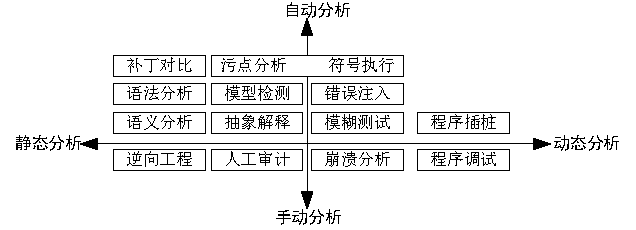
\includegraphics[scale=0.3]{chap01/根据挖掘方式分类}
\end{center}
\caption{根据挖掘方式分类}
\label{根据挖掘方式分类}
\end{figure}


\begin{figure}[htb]
\begin{center}
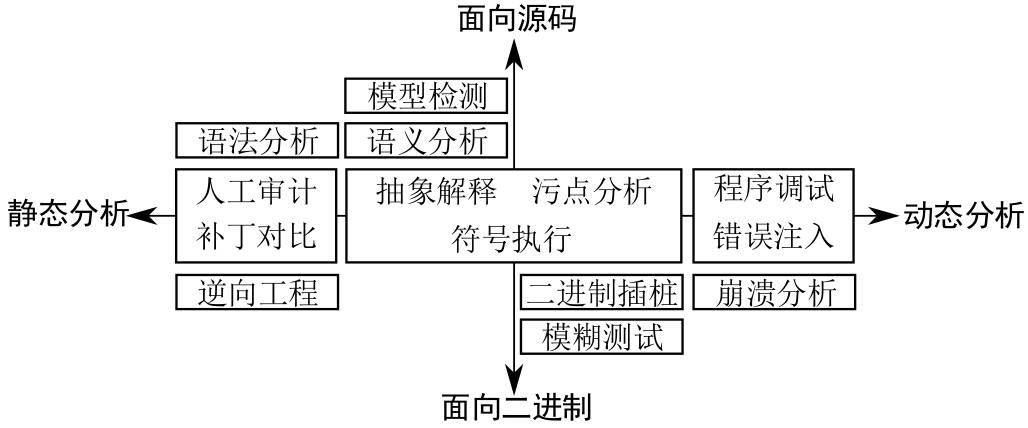
\includegraphics[scale=0.3]{chap01/根据挖掘软件类型分类}
\end{center}
\caption{根据挖掘软件类型分类}
\label{根据挖掘软件类型分类}
\end{figure}
%wb
\subsection{源代码软件静态挖掘技术}

静态挖掘技术是在不运行程序的情况下,自动的发现和报告潜在安全漏洞的技术的统称。静态分析能够全局的分析程序,不需要遍历每一个程序执行状态,从而扩大程序分析的规模。总体上,静态分析具有以下优点。(1)能够在软件生命周期的早期发现漏洞。静态分析可以在函数单元上进行单元测试,这使得错误可以在集成到大的代码模块之前被发现。进行单元测试之后,可以将精力集中在函数/单元之间的交互漏洞检测上,实现对源代码的分层检测。(2)能够检测大规模的软件。相对于人工审计,静态分析虽然压制了其报告解析能力,但是提高了检测特定漏洞的能力。相对于动态测试,不需要动态的遍历程序的每一个状态或者仅仅在源程序、中间表示上进行分析,能大大减少分析所需要的时间。同时静态分析也有以下不足。(1)在没有源代码的情况下,例如第三方库、操作系统等,静态分析需要猜测这些缺失的程序行为。(2)不能处理未域定义的程序错误行为。(3)不能检测运行时的漏洞、设计漏洞,系统管理以及由于用户的原因产生的漏洞。

%\begin{enumerate}[(1)]
%\item 能够在软件生命周期的早期发现漏洞。静态分析可以在函数单元上进行单元测试,这使得错误可以在集成到大的代码模块之前被发现。进行单元测试之后,可以将精力集中在函数/单元之间的交互漏洞检测上,实现对源代码的分层检测。
%\item 能够检测大规模的软件。相对于人工审计,静态分析虽然压制了其报告解析能力,但是提高了检测特定漏洞的能力。相对于动态测试,不需要动态的遍历程序的每一个状态或者仅仅在源程序、中间表示上进行分析,能大大减少分析所需要的时间。
%\end{enumerate}
%
%同时静态分析也有以下不足。
%
%\begin{enumerate}[(1)]
%\item 在没有源代码的情况下,例如第三方库、操作系统等,静态分析需要猜测这些缺失的程序行为。
%\item 不能处理未域定义的程序错误行为。
%\item 不能检测运行时的漏洞、设计漏洞,系统管理以及由于用户的原因产生的漏洞。
%\end{enumerate}

%大师兄
程序静态分析技术经过几十年的发展,形成了丰富的理论方法和技术手段,以程序静态分析为基础的静态漏洞挖掘方法的研究也极为深入。在词/语法分析、定理证明、抽象解释、符号执行、模型检验和机器学习等理论的支持下,静态漏洞挖掘取得了显著进展。
%大师兄

\subsubsection{词/语法分析技术}

词法分析通过对以往漏洞的分析,例如,人们发现缓冲区溢出常与某些语句或者语句组合有关(例如 strcpy, strcat),于是开发了一些通过词法分析发现缓冲区溢出漏洞的检测工具,例如 RATS\upcite{wnoauthor_cern_nodate}、 ITS4\upcite{noauthor_its4_nodate} 和Flawfinder\upcite{flawfinder_nodate} 等。此类工具对程序的语句进行遍历,并与预先建立的漏洞模式进行匹配,最后根据匹配结果报告可能的缓冲区溢出漏洞。由于这种方法不理解程序语义,所以容易产生漏报或误报。此技术一般只作为手工分析的起点。

\subsubsection{定理证明方法}

定理证明的基本思想是将源程序的语义和安全规范转换为逻辑公式,再将这些逻辑公式输入到一个定理证明器进行验证,从而将软件错误的发现过程转换为逻辑公式的证明过程。这种方法的优点是严格,能够保证通过验证的程序不存在漏洞,但它通常要求用户( 用形式逻辑语法) 提供循环不变式、过程调用的前置条件和后置条件等信息,以帮助定理证明器完成推导,因而难以实现自动化。Compaq 公司的 ESC\upcite{leino_esc/java_2000}、以色列 Tel-Aviv 大学的 CSSV\upcite{dor_cssv:_2003} 都采用定理证明方法检测程序中的缓冲区溢出漏洞。

\subsubsection{抽象解释技术}

抽象解释把程序的执行过程看成抽象状态的迁移过程,并通过抽象状态的分析确定程序的性质。为了保证分析结果的正确性,抽象解释要求初始抽象状态是初始实际状态的安全近似,且每次状态迁移都能保持正确关系。正确的抽象解释能够发现程序中的漏洞,但存在较多的误报,所以在实际使用时常常要求用户根据被测试程序的特性,选择合适的抽象域、加宽操作和解释函数等,以降低误报率。例如, Patrick Cousot 领导的项目 ASTREE\upcite{cousot_astree_2007} 采用基于抽象解释理论的程序静态分析器。ASTREE 可以检测数组越界访问、除零异常、浮点运算溢出和整数运算溢出等问题。ASTREE曾用于检验法国空中客车公司的空中巴士A340和A380系列飞机飞行控制软件,受到工业界的认可。除了ASTREE,FLUCTUAT\upcite{delmas_towards_2009} 、Coverity\upcite{almossawi_analysis_2006} 等都是采用抽象解释理论进行静态
漏洞检测的典型工具。抽象表达提供了对变量边界值的估计,但无法有效追踪变量之间的约束关系,在路径可行性判定上依然存在不足。

%\subsubsection{约束分析}
%
%约束分析是一种通过建立和求解程序的约束条件,发现程序性质的方法。基于约束分析的静态方法常将检测过程分为约束产生和约束检查两个独立步骤,前者利一组约束产生规则建立程序的约束条件,后者对建立的约束条件进行求解,进而检验程序的性质。约束分析可以处理无穷系统,而且自动化程度较高。美国加州大学Berkeley分院的 Wagner设计了一个基于约束分析的缓冲区溢出漏洞检测器BOON\upcite{noauthor_boon_nodate}。

\subsubsection{静态符号执行技术}

静态符号执行是King等人1976年在文献\upcite{king_symbolic_1976}一文中首先提出。符号执行的基本思想是,用抽象的符号表示程序中变量的值,根据程序的语义,遍历代码执行空间,来模拟程序的执行。符号执行的主要优势在于能够发现变量之间运算关系,便于理解程序的内在逻辑;在漏洞挖掘时,有利于在复杂的数据依赖关系中发现数据之间本质的约束关系,而且符号执行精确记录了路径的约束条件,可以进一步用于判断路径可行性和路径约束的完备性。

符号执行技术通过将程序的输入由具体值替换为符号变元,将程序中每条指令本身的具体计算语义映射为相应的符号计算语义,在程序控制流指导下,关注路径的分支谓词,为路径状态树中的每个叶子节点对应的程序路径推导出相应的能够到达该位置的敏感输入满足的最弱前条件。符号执行的核心,在于以等价类的形式对程序的执行路径进行标注,进而高效率地实现路径覆盖。

符号执行可以分析代码的所有语义信息,也可以只分析部分语义信息。符号执行分为过程内分析和过程间分析(又称全局分析)。过程内分析是指只对单个函数的代码进行分析,全局分析指对整个软件代码进行上下文敏感的分析。所谓上下文敏感分析是指在当前函数入口点要考虑当前的函数问调用信息和环境信息等。程序的全局分析是在过程内分析的基础上进行的,但过程内分析中包含了函数调用时就也引入了过程问分析,因此两者之间是相对独立又相互依赖的关系。

符号执行常常在对路径敏感的程序分析中使用。符号执行可以看作是程序测试与程序验证的折中方法,其优点在于它可以精确地静态模拟程序的执行。由于它跟踪了变量的所有可能取值,因此能够发现程序中细微的逻辑错误。但是在处理大程序时,程序执行的可能的路径数目随着程序尺寸的增大而呈指数级增长。在这种情况下需要对路径进行选择,选取定数量的路径进行分析。

早期静态符号执行典型系统包括Prefix\upcite{bush_static_2000}和ESP\upcite{das_esp:_2002}。W.Bush等人在1998年提出了Prefix,并在美国申请了若干专利。微软公司于1999年收购了Prefix,在Prefix基础上实现了Prefast。Prefix/Prefast已经成为微软内部标准源代码静态检验工具之一。ESP借鉴了MC由用户制定检查规则的思想,基于符号执行技术识别和保留路径上安全属性状态相关的约束条件,能够有效排除很多不可行路径。

\subsubsection{模型检测技术}

模型检验是一种针对有限状态并发系统的自动分析与验证技术,其基本思想是状态搜索。对状态空间的穷尽搜索有赖于对系统建立的有穷状态模型,以保证搜索过程的终止。模型检测的优点是能够做到完全自动化,在搜索终止时,如果性质没有满足,能够给出反例,这有利于用户对系统进行改进; 缺点是建模比较困难,且面临状态空间爆炸的问题。一般情况下,模型检查只适合用于对临时属性(如内存是否被释放、指针是否为空等)的检测。

模型检验技术最早应用于时序电路和通信协议设计的自动化检验,其基本思想是用状态迁移系统描述程序的行为,用时序逻辑、计算树逻辑或π演算公式表示系统的性质,从而将系统属性的检验问题转换为搜索不满足逻辑公式的状态系统的问题。模型检验需要遍历系统的整个状态空间,所以只能分析有限状态系统。例如,Berkeley大学的MOPS\upcite{chen_mops:_2002}、微软研究所的SLAM以及Bell实验室的UNO\upcite{holzmann_static_2002}都是基于模型检验的检测工具,它们能够发现程序中的一些字符串库函数的滥用。MOPS系统能够做到检测结果无漏报(完备性),但是MOPS是数据流不敏感的分析,无法跟踪数据依赖关系,导致MOPS误报率很高。SLAM\upcite{noauthor_slam_nodate}是一种基于谓词抽象技术的软件模型检验器,主要用于检测Windows操作系统驱动程序是否满足用户定义的属性约束。SLAM的核心技术是谓词抽象,将每个变量都抽象为只有0/1两种取值。这种过近似(Over Approximations)抽象方法导致SLAM误报较为严重。由于模型检验技术面临着状态空间爆炸的问题,在大型复杂软件的漏洞挖掘工作中仍处于探索阶段。

有些模型检验工具,例如Spin\upcite{noauthor_spin_nodate}与CBMC\upcite{noauthor_cbmc_nodate},能够直接应用于源代码,准确地捕捉程序的真实行为,精确度比较高。但是,它们要么可扩展性不好,不能应用于大规模的程序(如Spin);要么只能检查大型程序的部分状态,用作一种查错工具,不能覆盖所有的状态,不能保证找到所有的错误。另外一些模型检验工具基于谓词抽象的思想自动化抽取系统的有穷状态模型,如BLAST\upcite{beyer_software_2007}和SATABS等,它们的基本思路都是谓词抽象与CEGAR(Counter Example Guided Abstract Refinement,反例制导抽象精化)\upcite{andraus_cegar-based_2007},这也是目前主流的软件模型检验实现思路,但谓词发现以及模型精化仍是此类技术中的难点问题。


\subsubsection{基于机器学习的软件漏洞静态挖掘技术}
%随着机器学习算法的成熟,机器学习的很多方法也应用到了漏洞挖掘和软件测试之上。例如智能优化算法在模糊测试技术上的应用,AFL-go\upcite{bohme_directed_2017}利用模拟退火算法随着时间的推移分配种子变异的能量;AFL\upcite{noauthor_american_nodate}利用遗传算法框架变异种子以扩大测试的代码覆盖率;另外还有将遗传算法应用到回归测试\upcite{doungsa-ard_automatic_2007}、基于模型的模糊测试技术\upcite{sharma_applying_2014,sabharwal_prioritization_2010,you_genetic_2012,patton_genetic_2003}以及web测试\upcite{peng_new_2011}当中。

随着机器学习算法的成熟,一些研究者将机器学习的有监督、无监督算法以及神经网络算法和程序分析相结合用于挖掘软件漏洞。Padmanabhuni\upcite{padmanabhuni_predicting_2014,padmanabhuni_auditing_2016}利用有监督机器学习算法建立分类器用以检测缓冲区溢出漏洞。Neuhaus\upcite{neuhaus_predicting_2007}根据Mozilla的漏洞历史,从中提取向量,并利用机器学习算法预测哪些组件有可能出现漏洞。Zimmermann\upcite{zimmermann_searching_2010}以代码复杂度、代码混淆度等为特征预测Windows Vista中可能出现漏洞的组件。Perl\upcite{perl_vccfinder:_2015}利用github提交代码的语言类型、贡献者的fork数量等特征预测哪些提交可能出现漏洞。Grieco\upcite{grieco_toward_2016}以C语言程序中的函数调用轨迹为特征预测大规模程序中的漏洞。Yamaguchi\upcite{yamaguchi_chucky:_2013,yamaguchi_automatic_2015}利用异常检测检测源代码中缺少边界检测的情况以及使用聚类算法检测Taint-Style类型的漏洞。Rajpal\upcite{rajpal_not_2017}提出了一种基于时间递归神经网络的提高模糊测试代码覆盖率的方法。


\subsection{源代码软件动态挖掘技术}

动态测试是对程序运行时特性的测试分析,有别于静态分析检查源程序的手段,动态分析通过检查运行时的程序来获取程序特性。静态分析的结果通常对于每次程序的执行都成立,而动态分析的结果可能只对某一次或某几次运行成立。动态分析正在被广泛应用于包括系统安全分析在内的多个领域,软件工程国际会议(International Conference on Software Engineering/ICSE) 专门设立了动态分析研讨会( Workshop on Dynamic Analysis/WODA),会议的主题包括动态分析的各种研究和应用。

\subsubsection{运行时监测技术}

运行时监测(Runtime monitoring)是根据插桩的安全规范代码和检测代码在程序运行时检测是否违反安全规范。如斯坦福的Michael Martin等人的PQL(program query language)\upcite{martin_finding_2005},首先使用上下文敏感、流不敏感、基于包含的指针别名分析,找出所有可能的匹配点,然后对这些匹配点进行插桩后在运行时监测。另外像VS.Net 中使用的放在调用栈中的canary,canary值存放在用户数据和返回地址之间,一旦发现canary值被改变,则表明发生了缓冲区溢出。运行时监测首先要利用各种静态分析技术(如指针分析、别名分析、类型推断等),结合给出的安全规范,找出程序中所有可能违反安全规范的地方;然后利用代码插桩技术(包括静态插桩和动态插桩)对可能出现安全漏洞的地方插桩检测代码,同时插桩安全规范;最后利用动态检测算法在运行时检测程序是否违反安全规范。

\subsubsection{动态符号执行技术}

%\textbf{参考directed Greybox Fuzzing的introduction中关于符号执行的介绍}

基于动态符号执行的漏洞挖掘,一般将关注的程序漏洞以符号断言的形式进行描述。对每条路径的符号分析过程中,在敏感的程序点处对漏洞断言的可满足性进行判定。如确定断言为可满足,即断定当前分析路径中存在该类型漏洞。近年来,该型技术得到了较为广泛的应用。

2005年,Godefroid等学者提出的DART\upcite{godefroid_dart:_2005}系统是最早的动态测试用例生成系统。DART首先生成一个随机值作为外部变量的初始化输入,且对每个外部函数都返回一个随机值,由于随机值不能确保对程序中的每条分支都能覆盖到,因此随机测试的覆盖率通常很低。然而,DART对输入的随机值进行符号化处理,即在随机化之后,这些变量被标记为符号变量。在遇到新分支时,一条路径约束通过不断收集执行过程中的约束来生成,而下一条路径则是通过对另一分支的约束取反来生成。如果一条路径不可求解,这个约束将用具体值代入,进行化简。DART的缺点时不能处理指针语义,无法分析C语言中常见的指针操作。

CUTE\upcite{sen_cute_2006}被定义为一个混合符号执行工具,即联合了符号执行与具体执行。与DART系统类似,CUTE允许用户通过指定代码来决定哪些输入可以被符号化,这使得任意外部用户输入都可以被替代。CUTE的路径遍历是通过插桩来实现的。与DRAT相比,CUTE最大的改进是能够处理指针操作和数据结构。

斯坦福大学的Engle等学者提出的EXE\upcite{cadar_exe:_2008}系统,用于组件测试,在动态收集路径可达约束信息方面和约束路径精确求解方面的贡献较为突出。EXE系统是一个源到源的编译器。该编译器将目标应用源码中的每一个赋值和运算前都插入对EXE系统符号化执行组件的函数调用,并在程序的分支语句前插入一段调用求解器代码,对当前分支条件进行求解并产生测试用例。这样,当被EXE编译后的程序真正执行时,真实的程序执行和符号化执行交替进行,并且符号化执行从程序的具体执行中获取所需运行时信息,以收集路径可达约束。此外,EXE系统实现了一个SMT求解器 STP,该求解器包含了BV理论、ARRAY理论和整数理论。由于路径可达约束的收集和约束求解都较为精确,EXE系统生成的测试用例软件缺陷的发掘效率较高。

KLEE\upcite{cadar_klee:_2008}系统是基于EXE系统的升级,该系统将EXE系统的源到源编译器变为LLVM编译器\upcite{noauthor_llvm_nodate}。KLEE系统纯符号化执行LLVM编译出的低级指令。这些改进使得KLEE系统可以更为普适地应用于各类LLVM支持的语言程序。KLEE同样需要完整源码支持。并且由于KLEE系统采用完全符号化解释执行每一条LLVM指令,测试性能低。

SAGE\upcite{godefroid_sage:_2012}系统是微软研究院研发的动态测试用例生成系统。与之前的系统不同,SAGE系统直接对二进制程序进行动态追踪并生成测试用例。该系统采用动态二进制指令追踪工具Nirvana,监控程序执行,追踪指令执行获得程序的执行流日志。然后再离线地对日志文件进行符号化分析执行,构建路径可达约束,以便为输入可控分支生成测试用例。与EXE系统不同,SAGE系统为了能够对大规模程序进行分析,采取了一系列的简化措施:(1)SAGE系统为了简化约束收集和求解的复杂性,忽略对非线性约束的收集与求解。(2)SAGE 系统不对程序中的指针进行分析。相对于EXE系统,以上简化措施一定程度上加快了SAGE系统对大型目标软件的测试用例生成速度,然而这却以损失测试用例对路径覆盖指导的精度为代价。SAGE系统生成的测试用例中有接近60\%的测试用例无法准确指导程序覆盖目标路径。此外,SAGE系统对日志中的所有指令流都采用完全符号化解释执行,导致符号化执行时间占全系统工作时间的25\%。这就抵消了部分由前面所述简化操作带来的性能提升。

伯克利大学的SmartFuzz\upcite{molnar_dynamic_2009}系统与SAGE系统类似,采用了基于Linux下的二进制指令追踪工具Valgrind追踪程序执行和在线约束收集方式。SmartFuzz系统仅支持整数溢出缺陷的发掘。

李根设计和实现了Hunter\upcite{hunter__2010}系统,提出了基于路径完备可达理论以及污点可控指针分析的算法,能有效覆盖基于攻击面污点输入可达的测试路径,由于采用了基于虚拟机平台的符号化执行及线程监控技术,具有良好的跨平台兼容性。

在符号执行的实际应用中,还面临这许多问题,比如符号执行的精度
问题\upcite{godefroid_higher-order_2011},复杂的输入格式问题\upcite{majumdar_directed_2007,godefroid_grammar-based_2008},路径爆炸问题\upcite{boonstoppel_rwset:_2008,godefroid_compositional_2010},符号指针问题\upcite{trtik_symbolic_2014}等。其中路径爆炸问题是一个符号执行研究的一个重要分支。其主要形成原因在于,每一个分支条件语句都可能导致当前路径再分支出一条新的路径进行分析计算,而这是以指数的形式增长的。尤其体现在程序中存在跳转谓词与输入变元相关的循环结构时。

当前的解决办法包括:为循环引入“执行计数变量”,通过进行“执行计数变量”与输入的关联和程序中的变量与“执行计数变量”的关联,实现将程序中“循环次数相关”的变量的值完全通过输入相关属性表达的抽象计算。作为一种
摘要计算技术,约减了循环处理中的分析计算量;在对大量实际应用程序分析的基础上,仅仅为输入的“长度”和“部分输入前缀字符”引入符号变元,进行符号计算。该方法理论上并不是完备的,但实际应用中能覆盖较多的缓冲区溢出情形;有些相关研究提出综合使用程序切片、抽象解释、循环不变量计算和循环单值识别等技术对循环执行次数的上界进行估算:利用程序切片获取与循环结束判断条件相关的变量和语句,进而在此基础上进行抽象解释,对相关变量的取值范围近似获取。在经过循环不变量分析和循环单值识别后,进一步剔出变量值域,最终获取循环次数的估计值。

Godefroid等在文献中通过为包含归约变量的输入相关的循环计算循环摘要\upcite{godefroid_automatic_2011},避免了对每条循环相关分支的分析。但仅仅适用于循环中变量与归约变量存在线性关系的情况下;瑞士的开源项目S2E\upcite{chipounov_s2e:_2011}提出了选择式符号执行的思路:仅仅对关注的程序部分(某一特定代码模块或访问某一特定数据的代码部分)进行符号执行,在关注的程序部分和不关注的程序部分之间,维护确保分析状态一致性的转换机制。

%\subsubsection{导向符号执行技术}

导向符号执行是符号执行中利用程序分析以及约束求解技术有效的搜索可能目标路径空间的一个方向\upcite{ma_directed_2011}。Haller\upcite{haller_dowsing_2013}提出了一种导向危险库函数以及危险操作的区域的符号执行方法。另外一些研究者将导向符号执行应用到程序补丁验证\upcite{bohme_partition-based_2013,marinescu_katch:_2013,miller_empirical_1990}、增加符号执行代码覆盖率\upcite{xu_directed_2010}、减少静态分析误报\upcite{christakis_guiding_2016}以及崩溃重现之上\upcite{jin_bugredux:_2012, ros_sler_reconstructing_2013}。但是导向符号执行是重量级的,需要大量的程序分析以及约束求解。

%\subsubsection{约束求解技术技术}
%
%使用动态符号执行进行测试数据生成的基础在于底层的约束求解技术一一预期的程序路径约束最终需要表达为约束求解器所识别的语言,并由其判断可满足性以及给出对应的数据样本。
%
%lp\_solve\upcite{buttrey_calling_2005}是一个开源的线性规划求解器,其可以求解纯线性、整型、半连续及Special Ordered Sets\upcite{beale_global_1976}模型。我们将路径约束的求解问题转化为了在路径约束变量上的线性规划问题。虽然lp\_solve的求解能力不足以覆盖一般程序中出现的所有运算操作,如乘法、除法、位运算,但是已经足够覆盖足够的范围,即并行化现有方法。
%
%另一方面,如果需要表达能力更强的约束求解器,则可以选择SMT(Satisfiability Modulo Theories)\upcite{ranise_satisfiability_2006}求解器。SMT问题是布尔可满足性问题的扩展,前者将后者公式中的布尔变量替换为了由不同底层理论(如整型、实数、位向量甚至是不同的复杂数据结构)所支撑的谓词。因而,相比其他可用于约束求解的技术而言,SMT求解器有着更加强大的表达能力。当前的SMT求解器可直接支持包含如数组、结构体、枚举量之类的真实程序中经常出现的数据结构的模型,而避免了由包含这些结构的程序路径约束向表达能力较弱的求解器语言转换时可能导致的语义丢失。
%
%STP(Simple Theory Prover,简单理论证明器)\upcite{noauthor_simple_nodate}是用于求解定长比特向量和一维数组的逻辑公式可满足性的决策程序。简单的说STP就是一种用于求解特定逻辑方程组的工具。STP有其自身的语言规范,包括提供的接口函数和语法规则。接口函数包括比特向量的拼接和抽取、移位、符号扩展、有符号和无符号的算术操作(加减乘除取模等)和逻辑位操作等。还提供了比特向量间的有/无符号比较谓词(大于等于小于)。
%
%只要符号执行提取的路径条件符合 STP 的语法规范,就可以利用 STP 进行求解,从而判断一条具体的路径是否成立,如成立,则可得到对应该路径的测试用例。

\subsubsection{模糊测试技术}

Miller等\upcite{miller_empirical_1990}在1991年首次提出了模糊测试的概念,目的是检测UNIX命令行工具程序的可靠性。因为事先不知道程序、输入的结构信息,最先的模糊测试被称为黑盒模糊测试。模糊测试通过不同的方式(例如比特反转、边界值替换、输入块删除和复制)变异程序输入,从而产生大量的畸形输入;然后将畸形输入反馈给程序执行,观察程序是否异常。这个简单且有效的方法奠定了模糊测试的基础。下面从三个方面概述模糊测试技术。

(1)基于模型的黑盒模糊测试技术

传统的黑盒测试\upcite{noauthor_zzuf_nodate}没有考虑输入的结构信息,以至于变异的绝大部分输入因为不符合正确的格式标准而只能检测程序的一小部分路径。这种情况导致了传统的黑盒模糊测试不能挖掘程序的深层次信息。为了解决这个问题,研究者提出了基于模型的黑盒模糊测试框架例如Peach\upcite{noauthor_peach_nodate}和Spike\upcite{noauthor_immunity_nodate}。本质上,当输入是有格式的文件数据或者协议数据时,测试用例变异需要保证程序输入能够满足格式规范,从而通过程序的格式检测。这种方法增加了生成的测试输入的有效性,从而能够测试更深更关键的程序状态。但是,有的文件或报文格式并未公开,如何获得准确的输入格式或者绕过对输入格
式的校验成为研究的重点问题\upcite{li_automatic_2011,kim_efficient_2011,gorbunov_autofuzz:_2010,lin_automatic_2010,wang_taintscope:_2010}。另外还有一些研究者将遗传算法应用到基于模型的黑盒测试技术当中\upcite{sharma_applying_2014,sabharwal_prioritization_2010,you_genetic_2012,patton_genetic_2003}。

%随着机器学习算法的成熟,机器学习的很多方法也应用到了漏洞挖掘和软件测试之上。例如智能优化算法在模糊测试技术上的应用,AFL-go\upcite{bohme_directed_2017}利用模拟退火算法随着时间的推移分配种子变异的能量;AFL\upcite{noauthor_american_nodate}利用遗传算法框架变异种子以扩大测试的代码覆盖率;另外还有将遗传算法应用到回归测试\upcite{doungsa-ard_automatic_2007}、基于模型的模糊测试技术\upcite{sharma_applying_2014,sabharwal_prioritization_2010,you_genetic_2012,patton_genetic_2003}以及web测试\upcite{peng_new_2011}当中。

(2)覆盖率导向的模糊测试技术

覆盖率导向的模糊测试是通过一系列方法增加种子语料库代码覆盖率的技术。其出发点是基于这样一个判断“如果要检测某个程序元素$e$中的漏洞,种子语料库中就必须要包含一个种子在程序执行时能够到达$e$”,这里$e$可以是一个语句、一个基本块或者其他的区域。在执行一个测试用例时,覆盖率导向的模糊测试工具\upcite{bohme_coverage-based_2016,noauthor_american_nodate,rawat_vuzzer:_2017,sparks_automated_2007,noauthor_libfuzzer_nodate}使用轻量级的代码插桩在运行时收集代码覆盖信息。AFLFast\upcite{bohme_coverage-based_2016}设计了一种路径概率计算方式,变异概率较低的路径对应的测试用例能触发更多的路径,从而增加代码覆盖率。同时,设计一种测试用例变异能量分配方式,驱动模糊测试多变异遍历概率低的路径。Vuzzer\upcite{rawat_vuzzer:_2017}为每一个基本块设置了一个权重,并且计算每条路径的权重,在模糊测试时着重测试更可能触发漏洞的路径。Sparks\upcite{sparks_automated_2007}使用了遗传算法的思想变异定长的种子语料库并根据输入数据格式以遍历更深的路径。

(3)目标区域导向的模糊测试技术

目标区域导向的模糊测试是指在指定目标区域的情况下,通过设定一系列标准,驱动模糊测试执行到目标区域的技术。Marcel Böhme在AFL的基础上开发了AFL-go工具\upcite{bohme_directed_2017}。该工具定义了每个测试用例和目标区域的距离,并设计一种基于模拟退火的能量分配策略,使得随着时间的增加到目标区域距离较小的测试用例变异次数增加,而到目标区域距离较大的测试用例变异次数减少,以此增加测试用例经过目标区域的概率。虽然AFL-go在一定程度上实现了导向性,但是其变异的方式依然是无序的。基于此分析,论文第五章提出了一种细粒度变异的导向模糊测试方法,根据关键字段权重变异测试用例以达到快速导向并发现更多漏洞的目的。

还有另外的研究者提出了基于污点分析的导向模糊测试技术\upcite{henderson_decaf:_2017, newsome_dynamic_2005}。该技术利用污点分析方法判断哪些字段对导向目标区域具有关键作用,变异这些字段产生的测试用例能够以更大的可能性遍历到目标区域。通过这种方式能够极大的减少需要遍历的程序状态空间。

%\upcite{meng_assisting_2017}

\section{源代码软件漏洞挖掘的关键问题}

%静态分析和动态分析是源代码软件漏洞挖掘的两个主要方向。
通过对比分析现有的源代码软件漏洞挖掘方法及工具,可发现源代码软件漏洞挖掘存在以下发展趋势\upcite{zhangliyong_2011}。%抄源代码安全性分析
\begin{enumerate}[(1)]
\item 从内置安全规则到可扩展安全规则。现在的源代码安全分析工具都会提供多种配置机制和接口,供分析人员根据实际需要编写程序实现自定义的安全分析\upcite{noauthor_code_nodate,ashcraft_using_2002}。
\item 从依靠抽象语法树的词法匹配的方式到到多中间表示混合匹配的方式。抽象语法树只能识别出程序中的敏感操作,且会产生大量的误报,将其他的中间表示形式,如控制流图和数据流图综合考虑能大大减少误报。
%\item 从单类型源代码漏洞分析到多类型漏洞分析。
\item 从单纯的程序员指导程序分析到以程序员为辅助的自动程序分析。程序员在安全分析中的参与比重越来越小。现在许多模型检测、抽象解释工具的使用,只需要程序员在可能发生漏洞的区域添加注释就可以完成。而另外一些分析工具\upcite{gregor_stllint:_2006,noauthor_splint_nodate},因为使用了更为复杂的语义提取方式,程序员的参与度进一步减少。
\item 使用形式化方法辅助软件测试。软件测试方法本质上是遍历程序状态空间,容易引起状态空间爆炸。形式化方法通过提供语义等价的程序转换,能够减少状态空间。将二者结合,能够发现软件测试检测不了的漏洞。
\item 使用源代码的直接或者间接信息辅助软件测试。越来越多的从源代码中获取的信息用于帮助符号执行、模糊测试等软件测试方法,例如程序的执行路径\upcite{marinescu_katch:_2013}、以及程序基本块的距离\upcite{bohme_directed_2017}。
\end{enumerate}

通过多年的研究,源代码软件漏洞挖掘在上述各方面取得了不少进展,但仍然有很多问题有待解决。

%漏洞挖掘的最终目的是产生能够触发软件漏洞的测试用例。一般而言,测试用例的产生需要动态遍历程序状态空间。但是随着软件规模的增加,程序状态空间会产生爆炸性的增长,使得遍历所有的程序空间变得不可行。现在主流的挖掘流程是首先利用静态程序分析标定可能出现漏洞的代码区域——可疑区域,然后动态测试这些代码区域,从而减少测试的程序状态空间。所以,
%可疑区域的标定和动态测试是源代码软件漏洞挖掘的两个重要研究内容。虽然国内外研究者在这两个方面提出了很多的方法,例如危险函数搜索、模式匹配用于标定目标区域,模糊测试、符号执行用于动态测试,但在实际漏洞挖掘的过程中,仍有许多问题待解决。
%大体上源代码软件漏洞挖掘的关键问题可以分为两大类:可疑区域的标定问题和动态测试问题。虽然国内外学者对可疑区域标定以及动态测试已经进行了多年的研究,但仍然存在很多问题有待解决。
%可疑区域的标定一般是根据某类漏洞的特征设计固定的漏洞模式,然后利用字符串匹配方法或者在中间表示上遍历进行,此方式误报率高且标定的漏洞种类单一。此外,对于缓冲区溢出这种成因比较复杂的漏洞,即使使用了多种
%主流的动态测试方法包括符号执行和模糊测试。符号执行本质上需要遍历所有的程序状态空间,具有典型的路径爆炸问题;模糊测试利用随机输入遍历程序状态空间,相对于符号执行代码覆盖率较低,不能有效覆盖可疑区域。
%符号执行具有典型的路径爆炸问题而模糊测试具有路径覆盖率低且无法导向问题。
%综上,源代码软件漏洞挖掘的关键问题可以分为三类:多种类漏洞可疑区域标定问题、符号执行路径爆炸问题以及模糊测试导向问题。

%因此如何利用静态分析方法粗定位漏洞区域、
%相对于二进制软件,源代码软件包含更多的信息,主要表现在源代码具有更多更精确的中间表示形式。利用
%所以高精度的静态分析和可控的动态挖掘技术是源代码软件漏洞挖掘的重要研究方向。从另一方面来讲,

%syf
%源代码软件漏洞挖掘技术经过多年的研究和发展,逐渐积累了丰富了理论知识,产
%生了很多可用于漏洞挖掘的技术手段,但从软件漏洞挖掘本身的特性和当前软件
%漏洞挖掘采用的技术手段的特性上看,仍然面对以下主要问题:
%syf

(1)多种类源代码软件漏洞精确静态挖掘问题

%单一的中间表示表达能力有限的问题
%wb
%静态挖掘出潜在的软件漏洞是漏洞挖掘的出发点。论文认为挖掘包括检测和
%挖掘两个层次。论文将只有在漏洞真实触发时才能准确判定漏洞的方法称为漏洞
%检测;将不需要真实触发漏洞就能准确判定漏洞的方法称为漏洞挖掘。
%wb
繁多的源代码漏洞种类给漏洞挖掘带来了困难。由于不同种类的漏洞具有不同的特 %copy from syf
征,现存的基于模式匹配的漏洞挖掘工具,一方面不能检测多种源代码软件漏洞,另外一方面则会造成很高的误报。例如对于基于抽象语法树匹配的缓冲区溢出漏洞检测,通过遍历所有程序语句的抽象语法树虽然可以找到所有的内存拷贝函数,但是无法探知程序中是否对内存拷贝操作进行了边界检测;另外,抽象语法树对于缓冲区循环写造成的缓冲区溢出漏洞则完全没有检测能力。而上述问题可以通过将抽象语法树、控制流图、数据流图结合来解决。所以,研究多种中间表示的聚合方式并在此之上研究各类源代码漏洞的挖掘方法是一个关键问题。

(2)机器学习算法和源代码软件漏洞挖掘的结合问题

一般的漏洞静态挖掘方法则局限于特定的漏洞模式,若模式限制条件过强,则漏报率较高;若限制条件过弱,则误报率较高。对于缓冲区溢出漏洞,影响漏洞的静态特征有很多种,漏洞的形成是多个特征综合作用的结果。在源代码中这些静态特征可以通过各种中间表示获取,若将漏洞挖掘转换成机器学习中的分类问题,则能从以往的漏洞数据中学习出规律,解决上述问题。因此如何将机器学习算法和漏洞挖掘结合也是一个关键问题。

%将机器学习算法结合到漏洞挖掘上,则能不局限于特定的漏洞模式,根据以往的漏洞和非漏洞程序学习出一个综合的分类模型。例如,对于缓冲区溢出漏洞,影响漏洞的特征有很多种,漏洞的形成是多个特征综合作用的结果。而一般的漏洞静态挖掘方法则局限于特定的漏洞模式,若模式限制条件过强,则漏报率较高;若限制条件过弱,则误报率较高。
%若将漏洞挖掘转换成机器学习中的分类问题,则能从以往的漏洞数据中学习出规律,解决上述问题。
%因此如何将机器学习算法和漏洞挖掘结合也是一个关键问题。
%面对检测对象,如何将漏洞挖掘问题转换成机器学习中的分类问题是是漏洞挖掘和机器学习结合的关键。所以面对特殊的缓冲区溢出漏洞,如何选取特征、选取哪些特征。
%也会造成漏报率较高的问题。每年都会有大量的漏洞被曝出,如何利用已知的漏洞并从中建立模型降低可疑区域标定的漏报率也是一个关键问题。


(3)源代码静态信息辅助的模糊测试导向问题

模糊测试已被证明是一种非常强大的软件漏洞测试方法,是工业界和学术界研究的热点。但是模糊测试同样有它的局限性,盲目的随机的变异测试用例很难到达测试程序的特定路径,导致一些漏洞很难被触发。而在源代码中,漏洞可疑区域及其与其他代码的距离信息可以通过静态分析获取。如何利用这些信息指导模糊测试,动态的测试目标区域也是一个关键问题

(4)符号执行循环程序引起的路径爆炸问题

动态符号执行作为典型的动态测试方法,在理论上能够有效遍历目标软件的 %wb
状态空间,从而深度挖掘软件中存在的漏洞。但实际检测中,随着程序规模增大,符号执行必然会引起路径爆炸。导致符号执行路径空间爆炸的一个非常关键的因素是程序中的循环语句。在分析循环程序时,符号执行每一次进入循环体内部,都需要构造两条分支路径,分别对应了循环条件为真或假的情况,导致分支路径总数目随着循环次数的增加呈指数级增加。在源代码基础上的形式化方法能够将循环语义等价的转化成一个顺序语句,以缓解循环引起的路径爆炸问题。所以如何将形式化方法和符号执行结合缓解路径爆炸也是一个关键问题。
。
%所以,如何利用模糊测试动态的产生测试用例到达可疑区域也是一个关键问题。

\section{论文的研究思路与主要研究内容}
%wb
源代码漏洞挖掘是一项系统性的工作,只有融合多种理论、方法和技术才能挖
出潜在漏洞。软件漏洞挖掘不只是经验性的工作,而应该作为系统性的工程
来考虑。源代码软件漏洞挖掘起源于程序分析与测试领域,虽然有许多理论方法
支撑,但是各种方法都有其局限性。使用单一挖掘方法来发现软件漏洞越来越难,
只有系统性地看待软件漏洞挖掘问题,才能有所突破。

随着软件安全工程的引入,很多曾经挖掘出大量有价值漏洞的方法与工具在挖掘漏洞方面的优势越来越不明显。需要借鉴这些方法经验,研究新的挖掘思路。论文的研究对象是C/C++源代码软件,不涉及其他内存安全的语言,例如java、C\#等。
%wb
论文系统的研究了现有的源代码软件漏洞挖掘基础理论和方法,理清了这些理论和方法的脉络关系,明确了这些方法的优点和不足,并在此基础上提出了论文的漏洞挖掘思路和方法。论文的基本思路是:首先针对现有的基于模式匹配的挖掘方法不能精确挖掘多种类源代码软件漏洞的问题,研究将抽象语法树、控制流图和数据流图三种中间表示聚合的方法,并利用遍历聚合后的表示形式——程序性质图,挖掘各类源代码漏洞;
其次,
%针对基于程序性质图挖掘缓冲区溢出漏洞时漏报率较高的问题,
针对缓冲区溢出漏洞静态挖掘方法精确度不高的问题,利用缓冲区溢出漏洞的程序静态特征,研究基于机器学习的缓冲区溢出漏洞挖掘方法,
%用以平衡漏报率和误报率;
提高挖掘精度;随后,针对符号执行的路径爆炸问题,研究结合静态程序分析的高效符号执行算法,以控制符号执行规模;最后,考虑到现有导向模糊测试方法不能细粒度导向的问题,在利用时间递归神经网络训练测试用例的关键字段、累积关键字段权重的基础上,研究细粒度变异的导向模糊测试技术,增强导向模糊测试的效率以及漏洞挖掘的能力。

主要研究内容包括:

(1)基于程序性质图的源代码软件漏洞挖掘方法研究

基于模式匹配挖掘多种类源代码漏洞必须结合多种中间表示形式。论文研究了多种中间表示聚合的方法。该方法利用语法解析器解析源代码,依次生成语法分析树、抽象语法树、控制流图、数据流图。在将抽象语法树、控制流图以及数据流图聚合成程序性质图的基础上,定义并利用程序性质图的各种遍历方法,挖掘多种源代码漏洞。

(2)基于有机器学习的缓冲区溢出漏洞挖掘方法研究

针对缓冲区溢出漏洞挖掘精确度不高的问题,利用缓冲区溢出漏洞的程序静态特征,研究基于有机器学习的缓冲区溢出漏洞挖掘方法。该方法将22种程序静态特征约简成7类,分别是sink类型、缓冲区位置、容器、索引/地址/长度复杂度、边界检测、循环/条件/函数调用深度以及是否输入可控。通过扩展的程序性质图检测缓冲区溢出漏洞的各种静态特征并将其向量化,利用有监督机器学习算法在已标签的训练集上训练分类器。此分类器可用于在新的源代码中挖掘缓冲区溢出漏洞。

(3)基于细粒度变异的导向模糊测试技术研究

针对导向模糊测试的测试用例变异具有盲目性的问题,研究了一种细粒度变异的导向模糊测试技术。
该技术首先利用导向模糊测试收集测试用例;然后利用时间递归神经网络训练出一个模型,用于判断哪些字段对靠近目标区域其关键作用,同时收集每个字段的权重;在动态执行测试用例之前,利用上述模型判断当前测试用例中哪些属于关键字段并根据字段权重进行定向的变异。本方法能够更细粒度的变异指定字段,很大程度上消除模糊测试变异的盲目性,从而提高导向模糊测试的效率。

(4)结合静态分析的高效符号执行技术研究

导致符号执行路径空间爆炸的一个非常关键的因素是程序中的循环语句。在分析循环程序时,符号执行每一次进入循环体内部,都需要构造两条分支路径,分别对应了循环条件为真或假的情况。分支路径数目随着循环次数的增加呈指数级增加。
针对上述问题,研究了一种基于抽象解释的高效符号执行技术。给定待分析的源程序,首先解析出程序的控制流图。区别于其他符号执行技术,新技术通过静态程序分析方法,从程序的控制流图中计算出循环程序的不变式,然后通过用循环不变式代替循环,形成新的控制流图。在新的控制流图上进行符号执行,将会大幅减少符号执行的路径数量。




\section{论文的组织结构}

论文的结构排如图\ref{论文的组织结构}所示。

第一章为绪论,介绍课题的研究背景与意义,概述软件漏洞挖掘领域的国内外研究现状与进展,阐述论文的研究思路和主要研究内容。

第二章介绍源代码软件漏洞挖掘的基础知识和动态符号执行测试方法。介绍的基础知识包括:源代码的四种中间表示形式、源代码漏洞分类以及静态程序分析的理论基础。

第三章介绍基于程序性质图的源代码软件漏洞挖掘方法。介绍将抽象语法树、控制流图和数据流图三种中间表示用性质图进行聚合的方法,并利用遍历聚合后的表示形式——程序性质图,挖掘各类源代码漏洞的方法。介绍了缓冲区溢出漏洞的程序静态特征以及基于机器学习的缓冲区溢出漏洞挖掘方法。此章节属于纯静态分析,并不能产生导致程序崩溃的测试用例,旨在为动态测试标定目标区域,缩小测试范围。

第四章介绍基于细粒度变异的导向模糊测试技术。介绍如何利用时间递归神经网络获取关键字段以及如何计算关键字段权重;介绍在动态测试时,如何利用关键字段以及关键字段权重进行细粒度变异。

第五章介绍结合静态程序分析的高效符号执行技术。介绍了基于抽象解释的静态程序分析技术,设计了基于静态程序分析的高效符号执行方法。


第六章总结全文,并展望继续研究的方向。


\begin{figure}[htb]
\begin{center}
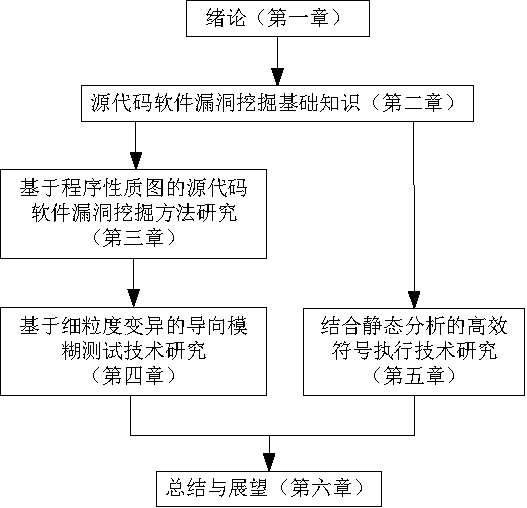
\includegraphics[scale=1.2]{chap01/论文的组织结构}
\end{center}
\caption{论文的组织结构}
\label{论文的组织结构}
\end{figure}

\chapter{源代码软件漏洞挖掘基础知识}

为了更好的介绍源代码漏洞挖掘后续章节研究工作,本章首先介绍了源代码的各种中间表示形式;其次,根据需要的中间表示数量的不同,给予源代码软件漏洞三种描述形式;然后,介绍了程序分析理论基础;最后,介绍了动态符号执行技术。

%常规软件测试方法用于分析源代码软件时尚有诸多问题需要探讨。漏洞挖掘的基本理论方法都源于程序分析与验证领域,尽管很多分析方法都得到了深入的研究,但这些方法通常单独或简单组合后被用于挖掘源代码软件中的漏洞,方法系统性的组合应用尚需要进一步摸索。因此,需要先理清不同分析方法的特点,找准其在系统性漏洞挖掘中的位置,为后续各章做铺垫。
%
%本章主要分析源代码软件测试的基础理论与方法,探讨了典型的静态程序分析、污点分析、符号执行和模糊测试等方法的基本原理及其在漏洞挖掘方面的应用。

\section{源代码中间表示形式}

因为源代码呈现出来的复杂性,在程序分析以及编译器设计技术里,研究人员提出了很多很多的中间表示用于表达程序。其中,语法分析树(Parsing Tree,PT)是语法解析器的直接产出结果。
%也是生成另外三个基本中间表示即抽象语法树(Abstract Syntax Tree,AST)、控制流图(Control Flow Graph,CFG)以及数据流图(Data Flow Graph,DFG)的基础。

\subsection{语法分析树}

语法分析树能够完全的反映程序语句的结构,以及如何将语句串联成一个完整的程序。输入一个程序,解析器根据语法文件辨别每一个终结符和非终结符,将这些标识符连接之后会得到语法分析树。语法分析树能够展示编程语言元素的类别、结构以及相互之间的关系,表现形式冗余性以及对微小改动非常敏感。图\ref{一个简单的实例程序}是一个简单的示意程序,变量x接受由外部输入函数fun得到的数据,y是x的乘法运算的结果,vul\_fun函数是一个漏洞函数。图\ref{语法分析树示例}是图\ref{一个简单的实例程序}的语法分析树示意图,其根节点是一个函数{(FUNC)},FUNC只有一个复合语句子节点{(CMPD)},复合语句包含两个语句{(STMT)}分别为赋值语句{(ASSIGN)}和跳转语句{(IF)}。


\begin{figure}[h]
\begin{lstlisting}[language=C]
void fun()
{
	int x = input();
	if(x < MAX)
	{
		int y = 2 * x;
		vul_fun(y);
	}
}
\end{lstlisting}
\caption{一个简单的实例程序}
\label{一个简单的实例程序}
\end{figure}


\begin{figure}[htp]
\centering
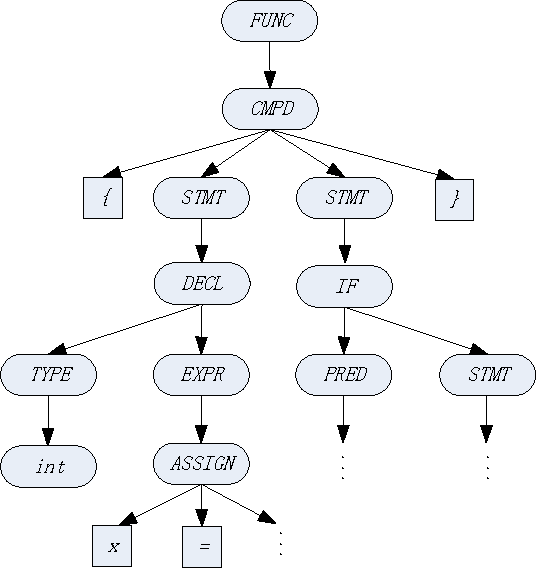
\includegraphics{语法分析树示意图}
\caption{图\ref{一个简单的实例程序}的语法分析树}
\label{语法分析树示例}
\end{figure}

\subsection{抽象语法树}

抽象语法树是语法分析树生成的最基本的中间表示,也是生成其他中间表示的基础。抽象语法树详尽的展示了操作数和操作符如何组成程序表达式以及语句,进而展示程序的整体形式。不同于语法分析树,抽象语法树不讲究和程序的每个token表示完全一致,其更偏向于语义的相似性。例如,两个用逗号隔开的变量声明将会产生两个连续的变量声明语法树。

抽象语法树是有顺序的树结构,内部节点是操作符(例如“+”和“=”)而叶子节点是操作数(例如常量和标识符)。图\ref{一个简单的实例程序}的抽象语法树如图\ref{抽象语法树示意图}所示。可以看出抽象语法树中删除了大括号和分号,另外函数调用节点{(CALL)}直接和赋值表达式相连,而语法分析树中在发现函数调用节点之前则需要遍历中间的所有节点。抽象语法树非常适合于简单的代码转换,经常被用来检验源代码的相似性\upcite{baxter_clone_1998,yamaguchi_generalized_2012}。但是抽象语法树不适用于更复杂的代码分析,例如死代码和以及未初始化的变量的检测,其原因是抽象语法树不能提供明显的控制流和数据流信息。


\begin{figure}[htp]
\centering
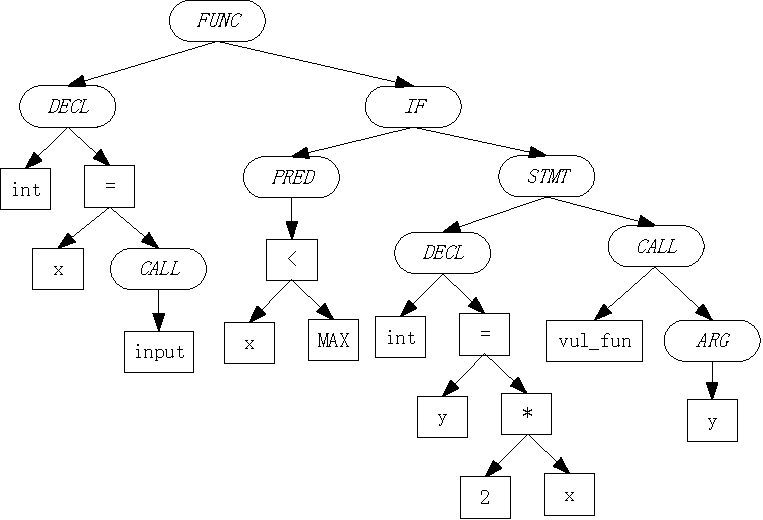
\includegraphics{chap02/抽象语法树示意图}
\caption{图\ref{一个简单的实例程序}的抽象语法树示意图}
\label{抽象语法树示意图}
\end{figure}

\subsection{控制流图}

控制流图能够描述程序语句的执行顺序以及为了执行某个语句哪些条件必须满足。无论是一般程序语句还是控制语句都用节点表示,节点之间用有向边连接以传递控制关系。相对于抽象语法树,控制流图的每条边都有一个标签$true$、$false$以及$true$分别表示控制语句的二类出边以及连接其他语句的边。图\ref{一个简单的实例程序}的控制流图如图\ref{抽象语法树示意图}所示。

控制流图在程序安全性分析中应用非常广泛,例如已知危险操作的变种\upcite{gascon_structural_2013}以及引导符号执行\upcite{sparks_automated_2007}等。另外,控制流图也已经被用在逆向工程中以帮助程序理解。虽然控制流图能够展示语句的执行顺序,但其不能提供数据流信息。在分析可疑漏洞时,不能判定某个语句是否可以被攻击者控制。

\begin{figure}[htp]
\centering
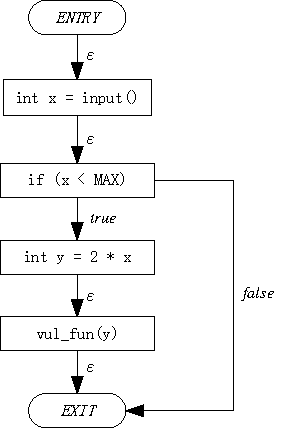
\includegraphics{控制流图}
\caption{图\ref{一个简单的实例程序}的控制流图}
\label{控制流图}
\end{figure}

\subsection{数据流图}

数据流图能够表示程序的语句之间数据依赖关系,数据流边连接的节点之间语句与语句之间的执行顺序。在数据流图上,可以不实际运行程序,直接考察数据的转移情况,从而获取数据流属性信息。图\ref{一个简单的实例程序}的数据流图如图\ref{程序数据流图}所示。变量x从声明语句传递到两个语句if(x<MAX)和int\ y = 2*x,变量y从声明语句传递到vul\_fun(y)。。

\begin{figure}[htp]
\centering
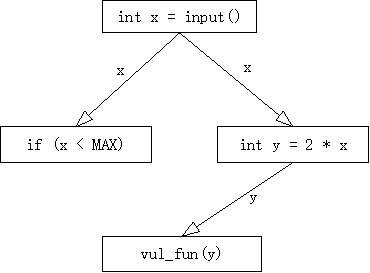
\includegraphics{chap02/程序数据流图}
\caption{图\ref{一个简单的实例程序}的程序数据流图}
\label{程序数据流图}
\end{figure}

\section{源代码漏洞描述}

源代码漏洞挖掘方法通常建立在不同的中间表示之上,根据描述源代码漏洞所需中间表示数量的不同,可以将源代码漏洞描述分为三类\upcite{yamaguchi_modeling_2014}:(1)基于抽象语法树的源代码漏洞描述;(2)基于控制流的源代码漏洞描述;(3)基于污染传播的源代码漏洞描述。不同种类不但描述的漏洞种类不同,而且对特定漏洞的描述精度也不相同。

\subsection{基于抽象语法树的源代码漏洞描述}

抽象语法树中可以获取源代码的每一个函数调用、语句甚至每一个操作数和操作符。所以利用抽象语法树可以获取攻击者可控的输入语句,敏感操作语句以及边界检测,但是不能检测出语句之间的关系。通过抽象语法树可以描述以下三类源代码漏洞:

\begin{enumerate}[(1)]
\item 不安全的参数使用。不安全的参数是引起源代码漏洞的一个重要原因。例如,格式化字符串漏洞的一个重要重要的一个特征是传递给$printf$和$sprintf$的格式化字符串受攻击者控制。所以若仅仅使用抽象语法树描述时,格式化字符串漏洞可以描述为“$printf$,$sprintf$,$fprintf$的格式化字符串不是常量”;
\item 整数溢出。当内存分配函数(alloc*)的表示内存分配大小的参数存在复杂算术运算时,整数溢出漏洞就有可能发生;
\item 数据类型错误使用。很多漏洞是由于数据类型不正确的转换引起的,例如,造成缓冲区溢出漏洞的一个重要原因就是缓冲区在初始化时,内存大小的运算未进行正确的转换和验证。在进行赋值操作时,如果右操作数的位宽比左操作数大则会发生整数截断。
\end{enumerate}

综上,下面给出基于抽象语法树的源代码漏洞描述。

\begin{definition}
\label{基于抽象语法树的源代码漏洞描述}
基于抽象语法树的源代码漏洞可以用一个二元组$(M_0,M_1)$表示,表示满足$M_0$而不满足$M_1$的所有的语句。其中,$M_0$和$M_1$表示两个谓词描述。
\end{definition}

利用抽象语法树挖掘源代码漏洞是非常有效的,但是其既不能完全表达攻击者可控的变量和敏感区域的关系。所以仅仅使用抽象语法树会产生非常多的误报。下一小节将会阐述控制流图是如何帮助部分的解决这个问题。

\subsection{基于控制流的源代码漏洞描述}

因为在控制流图中可以获取程序的执行顺序,很多源代码漏洞不但需要抽象语法树,还需要控制流图才能检测,具体漏洞类型如下所示:

\begin{enumerate}[(1)]
\item 内存泄露。很多漏洞的产生是因为分配的内存没有正确的释放。内存泄露会导致程序崩溃,另外也可以导致其他的漏洞;
\item UAF漏洞。若一个内存区域在释放后继续使用则会导致程序崩溃或者任意代码执行。此漏洞触发的主要原因是表面上无关的函数调用语句之间复杂的控制流交互关系。使用控制流分析可以轻易的得出内存释放和内存使用之间是否有控制依赖关系;
\end{enumerate}
上面两种情况,产生漏洞的原因都和控制流图上的某一条路径有关。例如,内存泄露是在一条控制流路径上内存被分配给一个变量,但在路径结束之前没有被释放而造成的。下面给出了基于控制流的源代码漏洞描述。

\begin{definition}
基于控制流图的漏洞可以用一个四元组$(S_{src},S_{end},S_{dst},\{(S^{i}_{cnd},t_i)\}_{i=1...N})$,其中$S_{src}$是一个基于抽象语法树描述的源代码语句,$S_{dst}$是目的语句,$\{(S^{i}_{cnd}),t_i\}$是过程中条件的语法描述和对应的结果,$t_i \in \{true, false\}$。一个语句$v$如果满足了以下三个条件:(1)$v$的语法树子节点中存在$v_{src}$与$S_{src}$想匹配;(2)在$v_{src}$和$v_{end}$之间存在一条控制流路径,且路径中不包含一个节点和$S_{dst}$相匹配,其中$v_{end}$是和$S_{end}$相匹配的语法树节点;(3)对于所有的$1< i \leq N$,若存在一个节点匹配$S^{i}_{end}$,则从此节点的所有出边的标记必须是$t_i$。
\end{definition}

控制流漏洞挖掘可以通过深度遍历从源节点到结束节点的所有路径,且结束节点不满足目的节点的描述,且中间节点必须满足相应的条件约束。但是仅仅使用控制流和语法树信息不能确定跟踪攻击者信息流,所以将在下一小节中介绍基于污染传播的源代码漏洞描述。

\subsection{基于污染传播的源代码漏洞描述}

基于污染传播的漏洞描述需要抽象语法树、控制流图以及数据流图三中中间表示形式。符合此标准的源代码漏洞包括:缓冲区溢出、缺乏权限检测以及代码注入等。例如,很多的缓冲区溢出漏洞产生的原因是内存拷贝函数中的长度参数没有被有效的验证;检测此类型漏洞就必须首先要获取内存拷贝函数调用的长度参数,然后利用控制流分析判断是否存在条件语句对长度参数做了有效的验证,同时还需要通过数据依赖关系分析判断长度变量是否和输入有数据依赖关系。下面给出了基于污染传播的源代码漏洞的形式化描述。

\begin{definition}
\label{基于污染传播的源代码漏洞描述}
基于污染传播的漏洞可以表示为一个三元组$(S_{src},S_{dst},S^{s}_{san})$,其中,$S_{src}$表示攻击者能够控制的输入语句,$S_{dst}$是导致漏洞的敏感操作,$S^{s}_{san}$是对应的边界检测。对于一个节点$v$,若$v_{source}$是满足$S_{src}$的一个语法树子节点,$v_{sink}$是满足$S_dst$的一个语法树子节点,且$v_{source}$和$S_{src}$满足以下个条件:(1)$v_{source}$和$S_{src}$之间存在一条数据依赖路径,即二者有数据依赖关系;(2)对于每一条数据依赖边$e_i = (v_i, v_{i+1})$,存在一条路径$(v_0,...,v_m)$且对于任意$v_k$不满足边界描述$S^{s}_{san}$,$0 \leq k \leq m$。
\end{definition}

\section{静态程序分析基础}

直观上,静态程序分析是指在不实际运行程序的前提下,对程序进行语义分析。
本节介绍程序的可达状态空间语义和不动点语义,二者是等价的。

\subsection{程序可达状态空间语义}

本节用符号$Var$指代程序变量的集合,符号$Func$指代函数的集合,
符号$Expr(Var, Func)$指代所有基于变量$Var$和函数$Func$构造的表达式,
如赋值表达式$x = y + f(z)$。
给定变量集合$Var$和函数集合$Func$, 用符号$Prog(Var, Func)$指代一段程序源代码。
在计算机中,程序源代码的的一般表示形式为控制流图(Control Flow Graph)。

\begin{definition}
给定程序$Prog(Var, Func)$,其控制流图定义为一个三元组$CFG_{Prog} = (L, E, l_0)$,其中,集合$L$表示是程序的所有控制节点,即源代码中程序指令位置;集合$E\subseteq L\times Expr(Var, Func) \times L$
	中的元素连接程序的控制节点,表示程序的控制流;$l_0$表示程序的初始节点。
\end{definition}


直观上,程序的控制流图是一个有向图,图的节点表示指令在源代码中的位置,
图的边表示程序的控制流,同时边上含有一个指令或者一个基本指令块。
一个简单的程序及其控制流图如图\ref{fig-example}所示。
节点$S1$表示程序的初始入口,边$(S1, x=0;n=100, S2)$表示程序文本中顺序执行的赋值指令序列。

\begin{figure}[h]
	\begin{minipage}{.5\textwidth}
		\centering
		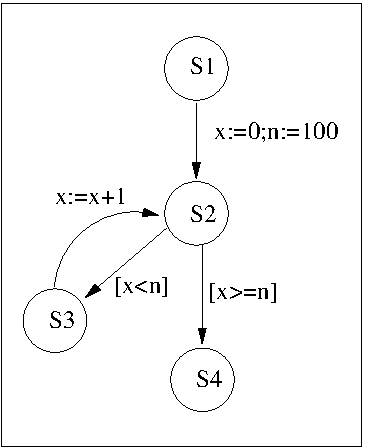
\includegraphics{figures/chap04/example1.pdf}
	\end{minipage}
	%
	\begin{minipage}{.5\textwidth}
		\centering
		\begin{lstlisting}
		int x,n;
		x=0;
		n=100;
		while(x<n)
			x=x+1;
		\end{lstlisting}
	\end{minipage}
	\caption{示例程序及其控制流图}
	\label{fig-example}
\end{figure}


控制流图存在其他的变种,例如编译器LLVM/Clang定义的控制流图将指令放在节点中。
但是,它们所定义的程序语义是等价的。程序的语义通常由状态迁移系统定义。

\begin{definition}
一个状态迁移系统可以定义为一个三元组$T=(S, R, S_0)$,其中,$S$是所有可能状态的集合(也称为状态空间);$R \subseteq S \times S $是迁移关系集合;$S_0$是初始状态集合。
\end{definition}


程序的状态空间由两部分构成:程序指令的位置和程序变量的取值。
给定程序变量集合$Var$,用符号$\textbf{Var}$表示变量所有可能取值集合,
那么,程序的状态空间可以表示为$S = L \times \textbf{Var}$,
其中,$L$是程序控制流图中的控制节点集合。
程序的状态空间可能是有穷集合,也可能是一个无穷集合,
如程序中含有整型变量时,其可能的取值范围为所有整数集合。
同理,程序的初始状态可能有无穷多个,如变量未初始化时。

迁移关系$R$定义了程序的进行一步操作时的状态变化过程,例如,
在图\ref{fig-example}所示程序中,
迁移$((S1, x=*, n=*), (S2, x=0, n=100))$
表示了程序在$S1$位置处执行赋值操作后,变量赋予相应的取值,
其中,符号$*$表示变量的取值为任意值。

一般地,程序的执行可以用一个迁移序列表示,例如,序列
$((S1, x=*, n=*), (S2, x=0, n=100),
(S3, x=0, n=100), (S2, x=1, n=100),
(S3, x=1, n=100) )$表示图\ref{fig-example}
中的程序从初始状态执行,并进入一次循环的状态变化过程。
为表述方便,本节用符号$r\in R$表示一个迁移,序列$r_0 r_1 \cdots r_n$表示一条迁移序列。

一个状态是可达的,当且仅当存在一条执行路径,使得程序能够从初始状态运行到达该状态。
形式化地,状态$s\in S$是可达的,当且仅当存在迁移序列$r_0 r_1 \cdots r_n$,
其中 $r_n = (s_n, s_{n+1})$,使得$s_0$为初始状态,且$s = s_{n+1}$。

给定一些错误状态,或者不安全的状态,
检测程序是否安全的问题可以归结为检测这些错误状态是否可达的问题,
即是否存在一条执行路径,使得程序能够从初始状态执行到某些错误状态。
因此,本质上,程序安全性分析问题可以归结为程序的可达状态空间遍历问题,
即通过遍历程序的所有可能状态空间,检测是否存在不安全的状态。


\subsection{程序不动点语义}

程序的可达状态集合通常是通过计算程序语义泛函的最小不动点得到。
该语义泛函是定义在程序状态迁移系统上的$Post$后继算子。


\begin{definition}
给定状态迁移系统$T=(S,R,S_0)$,
后继算子$Post: S \times R \rightarrow S$
是一个从状态空间和迁移关系到状态空间的映射。
给定状态集合$S_1 \subseteq S$,
$Post(S_1, R) = \{ s\in S | \exists s_1 \in S_1 \wedge (s_1, s)\in R \}$。
\end{definition}

与控制流图类似,后继算子也存在其他变种定义。
在程序分析中,后继算子通常也定义为从状态空间和程序指令到状态空间的映射,
即$Post: S \times Expr(Var, Func) \rightarrow S$。
通过将程序指令进行符号化编码(symbolic encoding),上述两个定义是等价的。
为表述方便,对上述两种定义不做区分。

直观上,给定程序的当前状态和迁移关系,
$Post$算子定义了在下一时刻,程序从当前状态执行一步迁移可能到达的状态集合。

$Post$后继算子作用在状态集合上。
一个状态集合称为程序语义的具体域中的一个元素。
因此,$Post$算子也可以看做是程序语义的具体域上的函数。
给定程序变量集合$Var$,以及变量可能取值集合$\textbf{Var}$,
程序的具体域为幂集$2^{\textbf{Var}}$。
可证后继算子是该具体域上的单调递增函数。

\begin{lemma}
$Post$后继算子是单调递增函数。
\end{lemma}

\begin{proof}
	假设状态集合$S_1 \subseteq S_2 \subseteq S$,
	证明义务为$Post(S_1, R) \subseteq Post(S_2,R)$。
	
	依据$Post$后继算子的定义,
	$Post(S_1, R) = \{ s\in S | \exists s_1 \in S_1 \wedge (s_1, s)\in R \}$,
	那么对任意$s\in Post(S_1, R)$,
	存在$s_1\in S_1$,使得$(s_1, s)\in R$。
	依据假设$S_1 \subseteq S_2$,得知$s_1 \in S_2$,
	故$s\in Post(S_2, R)$。
\end{proof}


一般地,从程序的初始状态,执行$n$次$Post$后继算子,
将得到程序执行$n$步可能到达的状态空间。
理论上,程序的可达状态空间可以通过$Post$后继算子进行数学刻画:
$Reach = \bigcup_{i=0}^{\infty}\{Post^{i}(S_0, R)\}$,
其中,$S_0$是程序的初始状态集合。
程序的可达状态空间可以通过不断迭代运用$Post$后继算子,
直至得到所有可能状态。
然而实际情况下,该迭代计算是不收敛的。
假设上述计算在迭代$n$次后终止,
表示程序的所有可达状态可以在$n$步计算内穷举,
第$n+1$计算不会产生新的状态,即$Post$算子存在不动点。


\begin{lemma}
程序的可达状态空间$Reach$等价于程序语义泛函$Post$算子的最小不动点,
即$Reach = LFP(Post)$。
\end{lemma}

由Knaster-Tarski不动点定理可知,	完备格上的单调函数存在最小不动点。
因此,如果程序语义的对象域构成一个完备格,并且程序的语义泛函是一个单调函数,
那么程序语义的最小不动点一定存在。
然而,即便理论上存在最小不动点,
该迭代过程的计算复杂度也随着程序规模的增长而呈指数级增长。
这就是通常所说的状态空间爆炸问题。

\section{动态符号执行技术}
%动态测试用例生成技术从2005年开始兴起,又被称为白盒Fuzzer。该技术以
%一组随机生成的数据作为输入,通过分析程序动态执行信息来获取可达路径对输
%入数据的约束,并在遇到受输入数据控制的分支跳转时将收集到的约束,输出至
%可满足模求解器(SMT Solver),用以判定另一分支路径是否可达。若可达,求解
%器则给出覆盖目标分支路径的测试用例,并利用生成的测试用例发掘目标分支路
%径中的软件缺陷。典型系统包括微软研究院的 DART\upcite{godefroid_dart:_2005}、 SAGE\upcite{godefroid_sage:_2012}、SmartFuzz\upcite{molnar_dynamic_2009}、 Hunter\upcite{hunter__2010}等。

%动态测试用例生成技术主要目标有两点:(1)为待测程序单元自动的生成可
%达到较高覆盖率的测试数据;(2)在动态过程中寻找待测程序的缺陷。

%作为动态测试用例生成技术的前身,传统的符号执行技术使用符号变量代替
%待测程序单元的实际输入值,之后使用替代的程序执行语义模拟执行待测程序单
%元。在执行过程中遇到的包含符号变量的条件表达式即为可决定程序执行路径的
%路径约束。待测单元的所有路径可通过对路径约束的真值赋值表示为一棵二叉执
%行树,其中每一个内部节点代表了一个分支路径选择。通过在树上深度优先的回
%溯搜索,寻找、判定预期路径约束的可达性并寻找对应的数据样本,满足预期执
%行路径的实际输入值即可被产生。但是,这种传统方法在处理大规模的或者较为
%复杂的待测单元时存在问题。例如,如果某一个路径约束的可满足性是无法判定
%的,那么传统的符号执行技术就无法继续进行搜索,从而导致了不佳的覆盖率;
%对于包含复杂数据类型(例如指针、数组)的程序,依靠静态的模拟执行无法精
%确的求解路径约束,同样也会在真实测试中导致低覆盖率。

动态测试用例生成技术的提出正是为了解决传统方法的不足,其基本想法在
于将传统符号执行中的符号输入与具体值输入相结合。动态符号执行采用实际输
入值真实地执行待测程序单元,在程序执行的过程中进行符号执行过程构建路径
约束,同时记录通过符号变量表达的抽象程序状态,以及用实际数值表达的真实
程序状态。由于待测程序被真实的执行了,所以所收集到的路径约束是遵循程序
本身的语义的,且是精确的。因而在动态方法中不会出现如静态方法的虚假警报,
并且也有助于对复杂数据结构进行分析处理。另外,由于程序的真实状态被记录,
一旦遇到不可判定的路径约束,可使用变量的实际值替代符号值,使后续的路径
探索过程可以继续进行。因为相比传统方法,可达到更高的覆盖率,所以其被广
泛的应用在了程序测试与验证中,并且有相当多的工作扩展了动态符号执行的适
用范围,如通过引入额外的内存模型以更精确的处理数组;通过引入额外的分析
方法提高对循环的覆盖率等。

动态测试用例生成技术的一般流程如图\ref{动态符号执行流程}所示。 其处理流程如下:
\begin{enumerate}[(1)]
\item 以某一具体输入启动目标程序, 该输入可随机生成;
\item 在目标程序的地址空间中,将输入对应的机器位置标记为符号变元;
\item 对目标程序的每条指令,将其计算语义提升到基于符号变元的符号表达式
域下,计算其抽象语义,更新对应的符号机器状态。对于符号计算相关的流程转
移类的指令,计算其对应于当前具体执行路径的分支谓词,累积至当前路径对应
的全局约束条件,同时计算另外一条分支对应的符号约束,通过约束求解进行可
满足性判断,确定该路径的可行性。在可行的情况下,将分支对应的路径约束保
存入调度队列;
\item 若调度队列非空,则从调度队列中抽取出一个分支约束,计算出满足约束
条件的输入的具体值,回到步骤 ① 对该路径进行符号分析;否则,即结束对目
标程序的符号分析。
\end{enumerate}

\begin{figure}[h]
\begin{center}
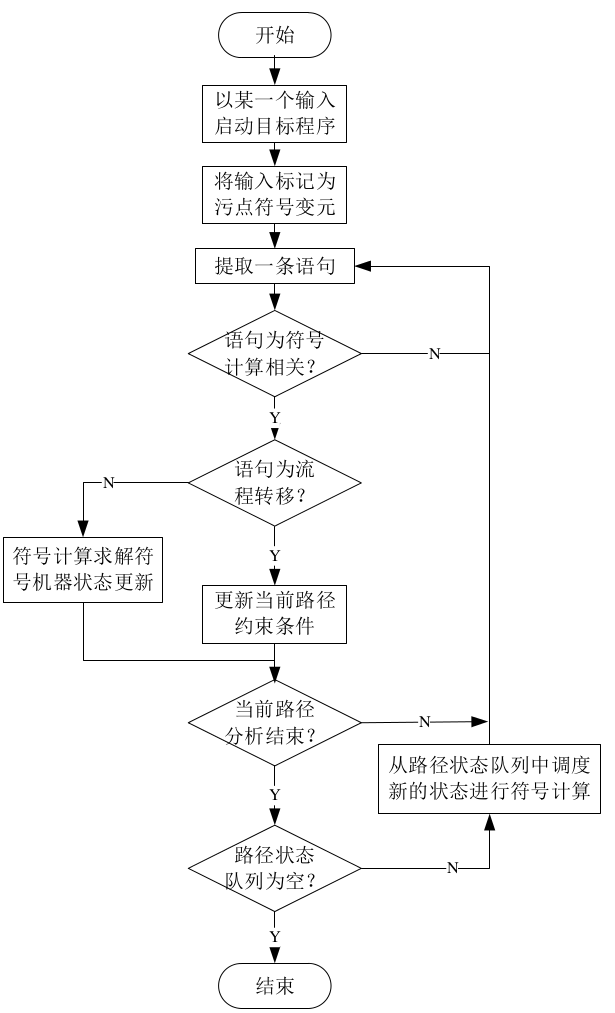
\includegraphics[scale=0.4]{chap02/动态符号执行流程}
\end{center}
\caption{动态符号执行流程}
\label{动态符号执行流程}
\end{figure}

论文第五章使用的符号执行工具是KLEE\upcite{cadar_klee:_2008}。KLEE是由Cadar与2008年开发的动态符号执行工具。KLEE依托于LLVM编译器,支持的最高的LLVM版本是3.4。KLEE执行LLVM字节码,记录程序中不同的路径,使用运行时检查器(Runtime Checker)检测程序错误,并利用约束求解器求解路径约束产生测试用例。KLEE能够获取很高的代码覆盖率并且发现深层次漏洞。

KLEE的架构如图\ref{KLEE架构}所示。和很多其他的符号执行工具一样,KLEE包含的一个主要的组件是metaSMT接口,支持多种约束求解器,例如Z3,STP,Boolector。KLEE还包含多种搜索策略即深度优先、宽度优先、随机搜索、最大覆代码覆盖率以及混合搜索策略,且提供了基本的搜索策略接口,可以方便的自定义搜索接口。此外,KLEE还实现了环境交互模型,即利用自己编写的数据读写函数代替程序原始调用的函数,例如open,read等。此做法有三个好处:(1)简化版的函数能够减轻原始复杂程序造成的路径爆炸;(2)能够根据代码规范模拟闭源的代码库,使得符号执行能够顺利执行;(3)通过模拟网络通信可以符号执行网络程序。尽管环境建模有这些优点,但是程序的模拟代码都是使用者手动编写的,每次遇到不同的程序需要重新编写。

\begin{figure}[h]
\begin{center}
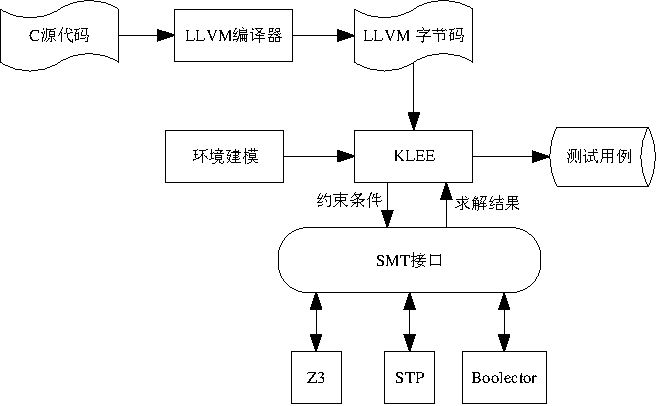
\includegraphics[scale=1.2]{chap02/KLEE架构}
\end{center}
\caption{KLEE架构}
\label{KLEE架构}
\end{figure}


%抄wb
%\section{模糊测试}
%模糊测试是指通过不断给目标软件发送各种畸形数据来挖掘其中可能隐含的
%安全漏洞,是一种强制性的漏洞挖掘方法。模糊测试与传统白盒方法不同,不需
%要分析程序源代码;也与传统黑盒测试只关注用例输出是否与预期相符有所不同,
%模糊测试只关注目标软件是否出现了异常\upcite{sutton_fuzzing:_2007}。
%
%\subsection{模糊测试的一般过程}
%具体模糊测试方法根据目标软件、输入格式、运行平台等不同的测试需求各
%不相同,但基本过程是一致的,包括以下几个步骤:
%
%(1)确定输入向量
%
%由于可利用漏洞都是由于软件在处理用户输入时没有经过正确的校验。因此,
%输入向量的枚举是模糊测试方法取得成功的关键因素。所有软件能够接收的数据
%都应该被认为是输入向量的组成部分,主要包括文件输入、网络数据包等。
%
%(2)生成测试用例
%
%在了解输入特性后,就可以根据变异或随机构造的方式生成测试用例。根据
%目标软件及其数据格式的不同,用例的生成方式也各不相同,可以采用随机生成
%的方式,也可以采用基于正常样本变异的方式,或者采用启发式规则生成的方式
%等\upcite{robertson_run-time_2003} 。一般模糊测试系统会生成海量测试用例,而其中大部分的用例都是无效
%的。因此,一般需要深入分析目标软件,构造更加有效的用例。
%
%(3)执行测试用例
%
%这一步通常与用例生成并行进行,执行过程一般包括启动目标软件、适用测
%试用例激励目标软件等。
%
%(4)异常检测与分析
%
%尽可能多地触发软件异常是模糊测试的目标。因此在测试目标软件时,应实
%时监测一切可能的异常、崩溃等信息,在异常发生时记录和保存重要的运行状态
%信息。并进一步分析软件异常的可利用性,合并重复的异常信息等。
%
%\subsection{测试用例生成方法}
%
%模糊测试是一种试图遍历软件输入空间的方法。因此,测试用例生成方法的
%好坏是影响模糊测试有效性的重要因素。测试用例生成方法大体上可分为两大类:
%基于变异的方法和基于生成的方法。
%
%(1)基于变异的方法
%
%这种方法从一个有效的输入样本开始,随机地变异样本中的部分数据来生成
%新用例。这是一个比较原始的方法,几乎不需要被测软件的任何先验知识,实现
%起来非常简单且通用性强。但这种方法效率很低,因为被测软件浪费了大多数的
%时间处理无效的输入数据。因此,后续有很多改进的方法,比如基于静态分析辅
%助的方法\upcite{wu_new_2009,lanzi_smart_2007,rawat_offset-aware_2011},基于运行时反馈方法 \upcite{ganesh_taint-based_2009,bekrar_finding_2011},基于遗传算法的方法\upcite{rawat_evolutionary_2010,liu_vulnerability_2008,cordon_ten_2004} 等。
%
%(2)基于生成的方法
%
%随机生成是最简单的生成策略,该方式只是简单地产生大量伪随机数据用于
%激励目标软件,能否触发异常有很大的概率性。因此,此法虽然简单却并不常用。预生成测试用例也是一种常见的生成策略,该方式首先研究目标软件的输入
%规范说明,以了解其支持的输入数据结构和取值范围,然后生成硬编码的畸形数
%据以测试边界条件或违反规约\upcite{liubiao__2014} 。这种方式生成的用例针对性强,因此测试效
%率相对较高。但是,创建这些用例需要事先完成大量的分析工作,自动化程度不
%高,而且有的输入规范并不可得。还有一种就是基于符号执行的生成方法,如
%SmartFuzz\upcite{molnar_dynamic_2009} 、SAGE\upcite{godefroid_sage:_2012} 等,这些系统将正常测试数据当作符号值,收集目标软件
%处理正常输入时的路径约束,通过约束求解生成新用例。理论上符号执行的方式
%能够生成精准的用例,但实际测试过程中由于面临路径爆炸、分析精度受限、指
%针分析难等问题,其应用场景也受到限制。
%
%\subsection{模糊测试框架}
%
%模糊测试框架是模糊测试过程的通用化实现。通过使用测试框架可以简化被
%测软件输入的表达、被测目标的监测和异常分析管理等,能够极大地提高模糊测
%试的自动化水平。虽然已经存在很多模糊测试框架,比如antiparser\upcite{noauthor_antiparser_nodate} 、
%Peach\upcite{noauthor_peach_nodate} 、Sulley\upcite{noauthor_sulley:_2017}、AUTODAFE\upcite{noauthor_autodafe_nodate} 等,但它们并不提供通用的解决方案,有其
%特定的适用范围。一般来讲,使用模糊测试框架可以实现功能复用,便于经验的
%积累和分享;但同时也必须花大量时间来学习框架,某些测试功能还可能因为框
%架的限制而无法实现。
%虽然模糊测试缺乏形式化模型和理论基础,然而模糊测试却是迄今为止发现
%未公开漏洞数量最多的挖掘方法。模糊测试实际上利用了漏洞挖掘问题的可猜解
%性和可验证性,虽然无法准确回答是否能检测到漏洞、是否能检测出所有漏洞等
%问题,却能够挖掘出很多意想不到的漏洞。因此,在其他挖掘方法效果不理想时,
%模糊测试可以作为一种很好的补充手段。论文在分析可编程类软件时,就采用了
%模糊测试的思想,基于模糊编程的思路对被分析软件进行测试。
%%抄wb

%\section{基于机器学习的漏洞检测方法}



\section{本章小结}

本章介绍了源代码漏洞挖掘中所使用的四种中间表示:语法分析树、抽象语法树、控制流图以及数据流图。在分析了各类中间表示表达能力的基础上,根据需要的中间表示数量的不同,将源代码软件漏洞描述为三类,即基于抽象语法树的源代码漏洞描述、基于控制流的源代码漏洞描述以及基于污染传播的源代码漏洞描述。最后,介绍了第五章所使用的静态程序分析基础以及动态符号执行技术。



%%% Local Variables:
%%% mode: latex
%%% TeX-master: "../main"
%%% End:

\begin{ack}
  行文至此,心中万分感慨。回顾博士阶段的五年学习生活,经历过认可时的激动和喜悦,也经历过失意时的苦涩和迷茫,少了一份功利,多了一份专注,这些带给我的不仅是科学思维上的磨练,更是全面素质的提升。在此,谨向多年来一直给予我知道、支持帮助的老师、同学和亲人们表示最衷心的感谢,是你们的陪伴和无私帮助激励我不断前行!
  
  衷心感谢我的导师沈荣骏院士。沈院士虽然不在长沙亲身知道,但定期他总要从北京赶来听取学生在课题方面的进展汇报,并给出很多建设性的意见和建议,来长沙出差之际,总是挤出时间和学生交流沟通。
  
  衷心感谢我的博士导师唐朝京教授!我从 2013 年受教于唐老师就读博士研究
  生至今,他严肃认真的治学态度、深厚的学术功底、严密的思维、渊博的知识和
  分析问题、提炼问题的能力,使我在学业上受益匪浅。我在博士论文选题、研究
  和论文写作的整个过程,都是在唐老师的悉心指导和严格要求下完成的。在几年
  的学习过程中,不仅使我的学术水平得到了很大的提高,在学术道德方面,我也
  有了更加深刻的认识,对自己的要求也更为严格。唐老师极富责任感、对待科研
  非常严谨,这种品质深深地影响着我,促使我形成严谨求实的学术作风,这将成
  为我人生的一大笔财富。唐老师还对我的论文写作方面进行了细心的指导,无私
  地传授给我论文写作的大量规律和经验。唐老师对工作认真勤恳的态度以及在学
  术上不断进取的精神永远是我今后工作学习的榜样!在此谨向他表示最衷心的感
  谢和最诚挚的敬意!
  
  衷心感谢张权副教授!是您带领我走进了信息安全研究的科研殿堂。感谢王
  剑教授、刘俭老师、张琛老师、张磊副教授、冯超老师、李瑞林老师等诸位老师对我的指导
  和关心。我在教研室学习期间,他们为我创造了良好的工作环境,他们在学术上
  的执着追求以及一丝不苟的工作作风也使我受
  
  感谢李孟君师兄、吴波师兄、解纬师兄、张博师兄、王少磊师兄、帅博师兄,王强师兄,感谢毕兴、刘毅、张斌、陈夏阳、叶嘉曦、张兴、冯冈夫、黄安琪、在同一个实验室中工作使得我们有了更多的讨论,在相互的交流和学习中我受益良多。
  
  深深的感谢我的家人,没有你们的支持,就没有今天的我!
  
  谨以此文献给所有关心我支持我的亲人和朋友们!

\end{ack}


%</thesis>
%    \end{macrocode}
%
% 在\LaTeX{}下管理参考文献将极其方便,建议使用Jabref生成条目,
% 用\verb|\cite|(其中\verb|upcite|是上标索引)索引即可。
% \verb|refs.bib|是你的参考文献名。
%    \begin{macrocode}
%<*thesis>
\cleardoublepage
\phantomsection
\addcontentsline{toc}{chapter}{参考文献}
\bibliographystyle{bstutf8}
\bibliography{ref/refs}

\begin{resume}

  \section*{发表的学术论文} % 发表的和录用的合在一起
%公开版
  \begin{enumerate}[{[}1{]}]
%  \addtolength{\itemsep}{-.36\baselineskip}%缩小条目之间的间距,下面类似
  \item Qingkun M, Chao F, Bin Z, Chaojing T. Assisting in Auditing of Buffer Overflow Vulnerabilities via Machine Learning.(SCI检索,检索号:00041904420001)
  
  \item Qingkun M, Shameng W, Bin Z, Chaojing T. Automatically Discover Program Vulnerability Through Similar Functions. PIERS2016.(EI检索,检索号20165203169818)
  
  \item Qingkun M, Bin Z, Chao F, Chaojing T. Detecting Buffer Boundary Violations based on SVM. ICISCE2016. (EI检索,检索号:20165003106907)
  
  \item Qingkun M, Shameng W, Chao F, Chaojing T. Predicting buffer overflow using semi-supervised learning. CISP-BMEI2016.(EI检索,检索号:20171303496365)
  
  \item Qingkun M, Shameng W, Chao F, Chaojing T. Predicting Integer Overflow through Static Integer Operation Attributes. ICCSNT2016. (EI检索,检索号:20180104610722)
  
  \item Shameng W, Qingkun M, Chao F, Chaojing T. Protocol Vulnerability Detection Based on Network Traffic Analysis and Binary Reverse Engineering. PLOS ONE, 2017. (SCI检索 000413195900048)
    
  \item Shameng W, Qingkun M, Chao F, Chaojing T. A Model-Guided Symbolic Execu-
  tion Approach for Network Protocol Implementations and Vulnerability Detection.
  PLOS ONE, 2017. (SCI检索,检索号:000413195900048)
  
  \item Shameng W, Chao F, Qingkun M, Bin Z, Ligeng W, Chaojing T. Testing Network
  Protocol Binary Software with Selective Symbolic Execution. CIS2016. (EI检索,检索号:20171203453840)
  
  \item Shameng W, Chao F, Qingkun M, Bin Z, Ligeng W, Chaojing T. Analyzing Net-
  work Protocol Binary Software with Joint Symbolic Execution. ICSAI2016. (EI检索,检索号:20171203462505)
  
  \item Shameng W, Chao F, Qingkun M, Bin Z, Ligeng W, Chaojing T. Model-Guided
  Symbolic Execution Testing for Network Protocol Binary Software. PIC2016. (EI
  检索,检索号:20173003971908)
  
  \item Shameng W, Chao F, Qingkun M, Bin Z, Ligeng W, Chaojing T. Multi-Packet
  Symbolic Execution Testing for Network Protocol Binary Software. ICCSNT2016.
  (EI检索,检索号:20180104611161)
  
%  \item 
  
  \end{enumerate}
  %盲评版
%  \begin{enumerate}[{[}1{]}]
%  %  \addtolength{\itemsep}{-.36\baselineskip}%缩小条目之间的间距,下面类似
%    \item 第一作者. Assisting in Auditing of Buffer Overflow Vulnerabilities via Machine Learning.(SCI检索,检索号:00041904420001)
%    
%    \item 第一作者. Automatically Discover Program Vulnerability Through Similar Functions. PIERS2016.(EI检索,检索号20165203169818)
%    
%    \item 第一作者. Detecting Buffer Boundary Violations based on SVM. ICISCE2016. (EI检索,检索号:20165003106907)
%    
%    \item 第一作者. Predicting buffer overflow using semi-supervised learning. CISP-BMEI2016.(EI检索,检索号:20171303496365)
%    
%    \item 第一作者. Predicting Integer Overflow through Static Integer Operation Attributes. ICCSNT2016. (EI检索,检索号:20180104610722)
%    
%    \item 第二作者. Protocol Vulnerability Detection Based on Network Traffic Analysis and Binary Reverse Engineering. PLOS ONE, 2017. (SCI检索 000413195900048)
%      
%    \item 第二作者. A Model-Guided Symbolic Execu-
%    tion Approach for Network Protocol Implementations and Vulnerability Detection.
%    PLOS ONE, 2017. (SCI检索,检索号:000413195900048)
%    
%    \item 第三作者. Testing Network
%    Protocol Binary Software with Selective Symbolic Execution. CIS2016. (EI检索,检索号:20171203453840)
%    
%    \item 第三作者. Analyzing Net-
%    work Protocol Binary Software with Joint Symbolic Execution. ICSAI2016. (EI检索,检索号:20171203462505)
%    
%    \item 第三作者. Model-Guided
%    Symbolic Execution Testing for Network Protocol Binary Software. PIC2016. (EI
%    检索,检索号:20173003971908)
%    
%    \item 第三作者. Multi-Packet
%    Symbolic Execution Testing for Network Protocol Binary Software. ICCSNT2016.
%    (EI检索,检索号:20180104611161)
%    
%  %  \item 
%    
%    \end{enumerate}

  \section*{参与的主要科研项目} % 有就写,没有就删除
  \begin{enumerate}[{[}1{]}]
  \addtolength{\itemsep}{-.36\baselineskip}%
  \item XXXX信息系统,海军项目,项目主要负责人.
  \item 全军XXXX装备业务系统,总参项目,项目主要负责人.
  \item XXXX挖掘验证测试技术,国家863项目,项目主要参与者.
  \item 大规模XXXX,2016国家重点研发计划,项目主要参与者.
  \end{enumerate}
\end{resume}

%</thesis>
%    \end{macrocode}
%
%<thesis>% 最后,需要的话还要生成附录,全文随之结束。
%    \begin{macrocode}
%<*thesis>
\appendix
\backmatter
% TeX
%\chapter{模板提供的希腊字母命令列表}
%
%大写希腊字母:
%\begin{table}[htbp]
%\centering
%\begin{tabular}{llll}
%\toprule
%$\Gamma$~\verb|\Gamma| & $\Lambda$~\verb|\Lambda| & $\Sigma$~\verb|\Sigma| & $\Psi$~\verb|\Psi| \\
%$\Delta$~\verb|\Delta| & $\Xi$~\verb|\Xi| & $\Upsilon$~\verb|\Upsilon| & $\Omega$~\verb|\Omega| \\
%$\Theta$~\verb|\Theta| & $\Pi$~\verb|\Pi| & $\Phi$~\verb|\Phi| & \\
%\midrule
%$\varGamma$~\verb|\varGamma| & $\varLambda$~\verb|\varLambda| & $\varSigma$~\verb|\varSigma| & $\varPsi$~\verb|\varPsi| \\
%$\varDelta$~\verb|\varDelta| & $\varXi$~\verb|\varXi| & $\varUpsilon$~\verb|\varUpsilon| & $\varOmega$~\verb|\varOmega| \\
%$\varTheta$~\verb|\varTheta| & $\varPi$~\verb|\varPi| & $\varPhi$~\verb|\varPhi| & \\
%\bottomrule
%\end{tabular}
%\end{table}
%
%小写希腊字母:
%\begin{table}[htbp]
%\centering
%\begin{tabular}{llll}
%\toprule
%$\alpha$~\verb|\alpha| & $\theta$~\verb|\theta| & $o$~\verb|o| & $\tau$~\verb|\tau| \\ 
%$\beta$~\verb|\beta| & $\vartheta$~\verb|\vartheta| & $\pi$~\verb|\pi| & $\upsilon$~\verb|\upsilon| \\ 
%$\gamma$~\verb|\gamma| & $\iota$~\verb|\iota| & $\varpi$~\verb|\varpi| & $\phi$~\verb|\phi| \\ 
%$\delta$~\verb|\delta| & $\kappa$~\verb|\kappa| & $\rho$~\verb|\rho| & $\varphi$~\verb|\varphi| \\ 
%$\epsilon$~\verb|\epsilon| & $\lambda$~\verb|\lambda| & $\varrho$~\verb|\varrho| & $\chi$~\verb|\chi| \\ 
%$\varepsilon$~\verb|\varepsilon| & $\mu$~\verb|\mu| & $\sigma$~\verb|\sigma| & $\psi$~\verb|\psi| \\ 
%$\zeta$~\verb|\zeta| & $\nu$~\verb|\nu| & $\varsigma$~\verb|\varsigma| & $\omega$~\verb|\omega| \\ 
%$\eta$~\verb|\eta| & $\xi$~\verb|\xi| & $\varkappa$~\verb|\varkappa| & $\digamma$~\verb|\digamma| \\ 
%\midrule
%$\upalpha$~\verb|\upalpha| & $\uptheta$~\verb|\uptheta| & $\mathrm{o}$~\verb|\mathrm{o}| & $\uptau$~\verb|\uptau| \\ 
%$\upbeta$~\verb|\upbeta| & $\upvartheta$~\verb|\upvartheta| & $\uppi$~\verb|\uppi| & $\upupsilon$~\verb|\upupsilon| \\ 
%$\upgamma$~\verb|\upgamma| & $\upiota$~\verb|\upiota| & $\upvarpi$~\verb|\upvarpi| & $\upphi$~\verb|\upphi| \\ 
%$\updelta$~\verb|\updelta| & $\upkappa$~\verb|\upkappa| & $\uprho$~\verb|\uprho| & $\upvarphi$~\verb|\upvarphi| \\ 
%$\upepsilon$~\verb|\upepsilon| & $\uplambda$~\verb|\uplambda| & $\upvarrho$~\verb|\upvarrho| & $\upchi$~\verb|\upchi| \\ 
%$\upvarepsilon$~\verb|\upvarepsilon| & $\upmu$~\verb|\upmu| & $\upsigma$~\verb|\upsigma| & $\uppsi$~\verb|\uppsi| \\ 
%$\upzeta$~\verb|\upzeta| & $\upnu$~\verb|\upnu| & $\upvarsigma$~\verb|\upvarsigma| & $\upomega$~\verb|\upomega| \\ 
%$\upeta$~\verb|\upeta| & $\upxi$~\verb|\upxi| & & \\ 
%\bottomrule
%\end{tabular}
%\end{table}
%
%希腊字母属于数学符号类别,请用\verb|\bm|命令加粗,其余向量、矩阵可用\verb|\mathbf|。


\end{document}
%</thesis>
%    \end{macrocode}
%
% 当然还有一些收尾工作,校验审阅自不必说。接下来你需要:修改论文中英文日期,
% 生成盲评,生成明(盲)评A3封面。
%
% {\color{blue}Happy \TeX{}ing! 欢迎提各式各样的意见!}
%
% \newpage\relax%
%
% \StopEventually{\PrintChanges}
% \clearpage
%
% \section{实现细节}
% 我们首先介绍文档模板的基本信息以及宏包和配置,
% 然后依照国防科技大学论文模板的书写规范一节一节的介绍实现步骤。
%
% \changes{v1.2}{2009/09/28}{添加了A3封面制作}
%
% \subsection{基本信息}
%    \begin{macrocode}
%<cls>\NeedsTeXFormat{LaTeX2e}[1999/12/01]
%<cls>\ProvidesClass{nudtpaper}
%<cfg>\ProvidesFile{nudtpaper.cfg}
%<cls|cfg>[2011/07/17 v2.2 NUDT paper template]
%    \end{macrocode}
%
% \subsection{宏包配置}
%
%<*cls>
%
%\changes{v0.99}{2009/08/17}{add package options}
% 当前的宏包选项在之前已经介绍了,下面是实现步骤,就是几个\verb|if|。
%\changes{v1.6}{2009/12/01}{添加单独的单双面控制}
%\changes{v2.0}{2010/11/09}{添加盲评控制}
%
%    \begin{macrocode}
\newif\ifismaster\ismastertrue
\newif\ifisttf\isttffalse
\newif\ifisfz\isfzfalse
\newif\ifisotf\isotffalse
\DeclareOption{master}{\ismastertrue}
\DeclareOption{doctor}{\ismasterfalse}
\newif\ifisanon\isanonfalse
\DeclareOption{anon}{\isanontrue}
\newif\ifistwoside\istwosidefalse
\DeclareOption{twoside}{\istwosidetrue}
\DeclareOption{ttf}{\isttftrue}
\DeclareOption{fz}{\isfztrue}
\DeclareOption{otf}{\isotftrue}
\newif\ifisvista\isvistafalse
\DeclareOption{vista}{\isvistatrue}
\DeclareOption*{\PackageWarning{nudtpaper}{Unknown Option '\CurrentOption'}}
\ProcessOptions\relax
%    \end{macrocode}
%
% 首先调用在文档类书写中需要的过程控制语句,在计算一些\verb|length|时要用到
%    \begin{macrocode}
\RequirePackage{ifthen,calc}
%    \end{macrocode}
%
% 接着我们导入文本类,该模板基于标准的书籍模板book,其默认格式为单面打印。
% 博士论文如需双面打印,必须指定\verb|twoside|选项。双开的含义是章节总是
% 起在右手边,左手空白页为完全的空白页,不包含页眉页脚。
%
% \changes{v1.6}{2009/12/01}{修改开关选项}
%
%    \begin{macrocode}
\ifistwoside
  \LoadClass[a4paper,12pt,openright,twoside]{book}
\else
  \LoadClass[a4paper,12pt,openany]{book}
\fi
%    \end{macrocode}
%
% 我们直接用\textsf{geometry}宏包进行页面边距的设定,调用titlesec设定标题以及页眉页脚,
% 用\textsf{titletoc}设定目录格式。需要改动的可以参考这三个宏包的说明文档。
%
%    \begin{macrocode}
\RequirePackage[includeheadfoot]{geometry}
\RequirePackage[center,pagestyles]{titlesec}
\RequirePackage{titletoc}
%    \end{macrocode}
%
% 文档中另外重要的两个部分是表格和图片。
% 首先来看图片:\textsf{graphicx}宏包是必不可少的,
% 并排图形。\textsf{subfigure} 已经不再推荐,用新的 \textsf{subfig}。
% 加入 \verb|config| 选项
% 以便兼容 \textsf{subfigure} 的命令。浮动图形和表格标题样式。\textsf{caption2} 已经不
% 推荐使用,采用新的 \textsf{caption}。它会自动被 \textsf{subfig} 装载进来。所以可以在
% 后面使用 \textbf{captionsetup} 命令,宏包\textsf{float}的作用是可以用H命令,
% 将浮动对象强制放在这里(副作用是版面可能不好):
%
%    \begin{macrocode}
\RequirePackage{graphicx}
\RequirePackage[config]{subfig}
\RequirePackage{float}
%    \end{macrocode}
%
% 再来看表格:我们采用\textsf{longtable}来处理长的表格,还需要\textsf{array}包;
% 标准的论文需要表格为三线表,这里引用\textsf{booktabs}宏包来处理,
% 这样,我们就可以简单的使用\verb|\toprule|,\verb|\midrule|,\verb|bottomrulle|
% 这样的命令;
% 为了在表格中支持跨行,需要引入\textsf{multirow}包,\textsf{tabularx}的作用是为了使用
% 固定宽度的表格,\textsf{slashbox}可以让我们在表格中使用反斜线:
%    \begin{macrocode}
\RequirePackage{array}
\RequirePackage{longtable}
\RequirePackage{booktabs}
\RequirePackage{multirow}
\RequirePackage{tabularx}
\RequirePackage{slashbox}
%    \end{macrocode}
% 表格和图片的例子可以搜索C\TeX{}论坛或者看示例文件。
%
% 引入\textsf{paralist}来达到比较好看的列表环境
%    \begin{macrocode}
\RequirePackage[neverdecrease]{paralist}
%    \end{macrocode}
%
% 文档中还需要一定的色彩控制和字体控制
%    \begin{macrocode}
\RequirePackage{xcolor}
%    \end{macrocode}
%
% 为了排出漂亮的数学公式,\textsf{amsmath}包是必不可少的,
% 需要注意的是,新版本的论文模板仍旧使用\textsf{txfonts}宏包,
% 为了支持希腊正体字母,需要调用\verb|upgreek.sty|,使用方法是\verb|\up<greek>|。
% 注意到这个宏包前面加上了\verb|Symbolsmallscale|选项,这是为了配合
% \verb|txfonts|希腊字体的大小而设定的。如果用户不满意这个宏包的积分号
% 等符号,倾向与使用传统的\LaTeX{}风格的数学符号,那么可以使用
% \textsf{mathptmx}宏包,但要把\verb|upgreek|的选项改为\verb|Symbol|,要不然
% 正体希腊字母要显得小一点哦。
% 而大写斜体希腊字母(变量)可以通过\textsf{amsmath}的\verb|\var<Greek>|得到。
% 当然,对于希腊字母的加粗推荐使用\verb|bm|宏包,一般变量的加粗那就使用
% \verb|\mathbf|吧!
% \changes{v2.0}{2010/11/09}{去掉fontspec,传递no-math到xeCJK,加入bm宏包}
% \changes{v2.2}{2011/07/16}{去掉txfonts宏包,使用lm字体,添加svgreek.sty}
% \changes{v2.2}{2011/07/16}{修改,仍旧使用upgreek, mathptmx, bm组合}
% \changes{v2.2}{2011/09/25}{修改,使用upgreek, txfonts, bm组合}
% \changes{v2.2}{2012/11/28}{给用户提供额外的选项,还是mtpro比较漂亮}
% \changes{v2.3}{2013/12/27}{调整数学字体,加入mtpro使用说明,并且仿照IEEE模板,修改displaypenalty}
%    \begin{macrocode}
\RequirePackage{amsmath,amssymb}
\RequirePackage{txfonts}
\RequirePackage[Symbolsmallscale]{upgreek}
%\RequirePackage{amsmath}
%\RequirePackage[amsbb,eufrak,compatiblegreek,subscriptcorrection,nofontinfo]{mtpro2}
\interdisplaylinepenalty=2500
\RequirePackage{bm}
\RequirePackage[T1]{fontenc}
\RequirePackage[amsmath,thmmarks,hyperref]{ntheorem}
%    \end{macrocode}
% 需要注意的是,如果用户有\verb|mtpro2|包,还是强烈建议使用这个的,因为数学公式
% 在这个包下显得特别的美观。虽然下载和安装不属于这篇使用说明的范畴,但是,上面的注释部分
% 可以给大家如何使用的一个简单的例子。当你安装好\verb|mtpro2|之后,主要取消注释,并且将
% 上面的三个包注释掉即可。
%
% 本文档类直接采用\XeTeX{}引擎,方便了字体配置以及编译,
% 这里需要调用\textsf{XeCJK}宏包,no--math的作用是不改变先前数学宏包设定的数学字体。
% 同时采用\textsf{indentfirst}宏包管理文字的缩进:
% \changes{v1.8}{2010/10/15}{修改了默认的xeCJK的选项,为了兼容旧的xeCJK版本,normalindentfirst选项暂不使用,而是在后面添加indentfirst包}
% \changes{v2.0}{2010/11/10}{传递no-math给xeCJK里面的fontspec宏包}
% \changes{v2.2}{2011/07/03}{移除CJKtextspace, CJKmathspace, CJKnumber选项}
% \changes{v2.4}{2015/02/09}{移除CJKnumber选项,添加新的CJKnum宏包。旧版本TexLive无需更改。}
%
%    \begin{macrocode}
\RequirePackage[CJKchecksingle,no-math]{xeCJK}
\RequirePackage{CJKnumb}
\RequirePackage{indentfirst}
%    \end{macrocode}
%
% 另外一个关键部分是文献索引,包括书签以及参考文献的索引,记得\textsf{hyperref}配合
% \XeTeX{}使用时暂不能开启Unicode选项,新的发行版已经移除\textsf{hypernat}包。另外还要注意,你最终的打印版肯定
% 不希望有花花绿绿的链接,对吧?那就把下面那行\verb|hyperref|注释掉就行了。
% \changes{v2.1}{2010/12/29}{移除hypernat包}
% \changes{v2.2}{2011/07/17}{移除hyperref的CJKbookmarks旋向}
% \changes{v2.3}{2013/12/27}{加入色彩版hyperref}
%    \begin{macrocode}
\RequirePackage[numbers,sort&compress,square]{natbib}
\RequirePackage[colorlinks=true,linkcolor=blue,citecolor=red,pdfborder=0 1 1]{hyperref}
%\RequirePackage[pdfborder=0 0 1]{hyperref}
%    \end{macrocode}
%</cls>
%
%\subsection{基础配置}
% 本章主要介绍模板中用到的基本的元素和定义,现在包括两部分: 字体,字号和字体命令
%
%\subsubsection{字体定义}
% 我们首先来处理\TeX{}中最令人棘手的字体问题,
% 在使用\textsf{XeCJK}包之后,配置和选择很容易,
% 预先设定好一些字体命令是为了后面方便的更改文本字体的需要。
% 首先我们开启\TeX{}连字符:
%    \begin{macrocode}
%<*cls>
\defaultfontfeatures{Mapping=tex-text}
%</cls>
%    \end{macrocode}
%
% 之后用\textsc{XeCJK}包提供的命令设定字体,用户可以选择使用TTF还是OTF字体,
% Adobe的OpenType字体在排版上更具备优势,文档显示锐利,推荐使用。
% 另外在这一个新版本中,我们推荐用户也可以使用方正的字体,只要使用\verb|FZ|选项即可。
% 中注释掉相关的字体就可以。方正字体的有点是标点符号的位置无需修正,且字体之间配合很好。
% \verb|setcharclass|的作用是纠正xunicode、xeCJK的一些设定:
%
% \changes{v0.99}{2009/08/17}{add options TTF and OTF}
% \changes{v0.993}{2009/08/25}{加入VISTA用户选项}
% \changes{v1.9}{2010/10/28}{定义一个cusong字体,使用的是中宋}
% \changes{v2.3}{2013/12/27}{用户可以考虑使用方正字体,加入FZ选项}
%
%    \begin{macrocode}
%<*cls>
\xeCJKsetcharclass{"0}{"2E7F}{0}
\xeCJKsetcharclass{"2E80}{"FFFF}{1}
\newcommand\installTTF{%
  \setmainfont{Times New Roman}
  \setsansfont{Arial}
  \setmonofont{Courier New}
  \ifisvista
    \setCJKmainfont[BoldFont={SimHei},ItalicFont={KaiTi}]{SimSun}
    \setCJKmonofont{KaiTi} % Pluto use LiSu Thu use Kaiti, orig is SimSun
    \setCJKfamilyfont{fs}{FangSong}
    \setCJKfamilyfont{kai}{KaiTi}
  \else
    \setCJKmainfont[BoldFont={SimHei},ItalicFont={KaiTi_GB2312}]{SimSun}
    \setCJKmonofont{KaiTi_GB2312} % Pluto use LiSu Thu use Kaiti, orig is SimSun
    \setCJKfamilyfont{fs}{FangSong_GB2312}
    \setCJKfamilyfont{kai}{KaiTi_GB2312}
  \fi
  \setCJKsansfont{SimHei}
  \setCJKfamilyfont{song}{SimSun}
  \setCJKfamilyfont{hei}{SimHei}
  \setCJKfamilyfont{li}{LiSu}
  \setCJKfamilyfont{you}{YouYuan}
  \setCJKfamilyfont{cusong}{STZhongsong}
}
\newcommand\installOTF{%
  \setmainfont{Times New Roman} % could be changed to "Times New Roman PS Std" !!
  \setsansfont{Arial}
  \setmonofont{Courier New}
  \setCJKmainfont[BoldFont={Adobe Heiti Std},ItalicFont={Adobe Kaiti Std}]{Adobe Song Std}
  \setCJKsansfont{Adobe Heiti Std}
  \setCJKmonofont{Adobe Kaiti Std}
  \setCJKfamilyfont{song}{Adobe Song Std}
  \setCJKfamilyfont{hei}{Adobe Heiti Std}
  \setCJKfamilyfont{fs}{Adobe Fangsong Std}
  \setCJKfamilyfont{kai}{Adobe Kaiti Std}
  \setCJKfamilyfont{li}{Adobe Kaiti Std}
  \setCJKfamilyfont{you}{Adobe Kaiti Std}
  \setCJKfamilyfont{cusong}{STZhongsong}
}
\newcommand\installFZ{%
  \setmainfont{Times New Roman} % could be changed to "Times New Roman PS Std" !!
  \setsansfont{Arial}
  \setmonofont{Courier New}
  \setCJKmainfont[BoldFont={FZHei-B01},ItalicFont={FZKai-Z03}]{FZShuSong_GB18030-Z01}
  \setCJKsansfont{FZHei-B01} % Hei
  \setCJKmonofont{FZKai-Z03} % Kai
  \setCJKfamilyfont{song}{FZShuSong_GB18030-Z01}
  \setCJKfamilyfont{hei}{FZHei-B01}
  \setCJKfamilyfont{fs}{FZKai-Z03} % Kai
  \setCJKfamilyfont{kai}{FZKai-Z03} % Kai
  \setCJKfamilyfont{li}{FZKai-Z03} % Kai
  \setCJKfamilyfont{you}{FZKai-Z03} % Kai
  \setCJKfamilyfont{cusong}{FZXiaoBiaoSong-B05} % 小标宋
}
\newcommand{\cusong}{\CJKfamily{cusong}} % 中宋作为加粗宋体
%</cls>
%    \end{macrocode}
%
% \changes{v1.6}{2009/12/01}{替换OTF英文字体为标准Windows自带字体}
% \changes{v2.3}{2013/12/27}{添加FZ字体选项}
% 之后我们根据你的设定决定安装什么字体:
%
%    \begin{macrocode}
%<*cls>
\ifisttf
  \installTTF
\else
  \ifisfz
    \installFZ
  \else
    \installOTF
  \fi
\fi
%</cls>
%    \end{macrocode}
%
% 选定好字体之后,就是设定字体别名,这样我们就可以在文档的其他部分直接使用较短的命令来
% 指定特定的字体了:
%
%    \begin{macrocode}
%<*cls>
\newcommand{\song}{\CJKfamily{song}}    % 宋体
\newcommand{\fs}{\CJKfamily{fs}}        % 仿宋体
\newcommand{\kai}{\CJKfamily{kai}}      % 楷体
\newcommand{\hei}{\CJKfamily{hei}}      % 黑体
\newcommand{\li}{\CJKfamily{li}}        % 隶书
\newcommand{\you}{\CJKfamily{you}}      % 幼圆
\def\songti{\song}
\def\fangsong{\fs}
\def\kaishu{\kai}
\def\heiti{\hei}
\def\lishu{\li}
\def\youyuan{\you}
%</cls>
%    \end{macrocode}
%
% \subsubsection{字号定义}
%下面就是定义字号大小,这一部分我们有两个参考,其一是:
%
% \begin{verbatim}
% 参考科学出版社编写的《著译编辑手册》(1994年)
% 七号      5.25pt       1.845mm
% 六号      7.875pt      2.768mm
% 小五      9pt          3.163mm
% 五号      10.5pt       3.69mm
% 小四      12pt         4.2175mm
% 四号      13.75pt      4.83mm
% 三号      15.75pt      5.53mm
% 二号      21pt         7.38mm
% 一号      27.5pt       9.48mm
% 小初      36pt         12.65mm
% 初号      42pt         14.76mm
%
% 这里的 pt 对应的是 1/72.27 inch,也就是 TeX 中的标准 pt
% \end{verbatim}
%
% 另外一个来自WORD中的设定:
% \begin{verbatim}
% 初号 = 42bp = 14.82mm = 42.1575pt
% 小初 = 36bp = 12.70mm = 36.135 pt
% 一号 = 26bp = 9.17mm = 26.0975pt
% 小一 = 24bp = 8.47mm = 24.09pt
% 二号 = 22bp = 7.76mm = 22.0825pt
% 小二 = 18bp = 6.35mm = 18.0675pt
% 三号 = 16bp = 5.64mm = 16.06pt
% 小三 = 15bp = 5.29mm = 15.05625pt
% 四号 = 14bp = 4.94mm = 14.0525pt
% 小四 = 12bp = 4.23mm = 12.045pt
% 五号 = 10.5bp = 3.70mm = 10.59375pt
% 小五 = 9bp = 3.18mm = 9.03375pt
% 六号 = 7.5bp = 2.56mm
% 小六 = 6.5bp = 2.29mm
% 七号 = 5.5bp = 1.94mm
% 八号 = 5bp = 1.76mm
%
% 1bp = 72.27/72 pt
% \end{verbatim}
%
% 我们采用习惯的字号设定方法(也就是WORD中的设定),首先编写字体设置命令:
%
%\begin{macro}{\choosefont}
% 我们可以使用 |\choosefont| 来选择字体, 字体设定这些大多是从清华的模板拷过来的。
%
%    \begin{macrocode}
%<*cls>
\newlength\thu@linespace
\newcommand{\thu@choosefont}[2]{%
    \setlength{\thu@linespace}{#2*\real{#1}}%
    \fontsize{#2}{\thu@linespace}\selectfont}
\def\thu@define@fontsize#1#2{%
    \expandafter\newcommand\csname #1\endcsname[1][\baselinestretch]{%
    \thu@choosefont{##1}{#2}}}
%</cls>
%    \end{macrocode}
%\end{macro}
%
%设定具体的字体大小:
%
%    \begin{macrocode}
%<*cls>
\thu@define@fontsize{chuhao}{42bp}
\thu@define@fontsize{xiaochu}{36bp}
\thu@define@fontsize{yihao}{26bp}
\thu@define@fontsize{xiaoyi}{24bp}
\thu@define@fontsize{erhao}{22bp}
\thu@define@fontsize{xiaoer}{18bp}
\thu@define@fontsize{sanhao}{16bp}
\thu@define@fontsize{xiaosan}{15bp}
\thu@define@fontsize{sihao}{14bp}
\thu@define@fontsize{banxiaosi}{13bp}
\thu@define@fontsize{xiaosi}{12bp}
\thu@define@fontsize{dawu}{11bp}
\thu@define@fontsize{wuhao}{10.5bp}
\thu@define@fontsize{xiaowu}{9bp}
\thu@define@fontsize{liuhao}{7.5bp}
\thu@define@fontsize{xiaoliu}{6.5bp}
\thu@define@fontsize{qihao}{5.5bp}
\thu@define@fontsize{bahao}{5bp}
%</cls>
%    \end{macrocode}
%
%\subsubsection{自定命令}
% 有一些常量,测试,自定义的命令等都放在这里,待到论文逐渐完善之后再做定夺,
% 当然用户自己的命令也可以在此添加,事实上如果natbib传递的是superscript,
% \verb|cite|命令默认就成了上标了。这里不加入这个选项,而是单独编写一个命令:
%
%    \begin{macrocode}
%<*cls>
\newcommand{\upcite}[1]{\textsuperscript{\cite{#1}}} % 上标形式引用
\newcommand{\china}{中华人民共和国}
\def\nudtpaper{\textsc{Nudt}\textsc{Paper}}
\newcommand{\pozhehao}{\kern0.3ex\rule[0.8ex]{2em}{0.1ex}\kern0.3ex}
%</cls>
%    \end{macrocode}
%
%\subsubsection{中文元素}
%
% 默认的页面元素的英文名,诸如Contents为目录,Abstract为摘要等,
% 我们首先将他们一一中文化:
% \changes{v0.992}{2009/08/19}{修改图表编号格式}
% \changes{v1.3}{2009/10/14}{修改图目录和表目录}
%
%    \begin{macrocode}
%<*cls>
\renewcommand\contentsname{目\hspace{1em}录}
\renewcommand\listfigurename{图\hspace{1em}目\hspace{1em}录}
\renewcommand\listtablename{表\hspace{1em}目\hspace{1em}录}
\newcommand\listequationname{公式索引}
\newcommand\equationname{公式}
\renewcommand\bibname{参考文献}
\renewcommand\indexname{索引}
\renewcommand\figurename{图}
\renewcommand\tablename{表}
\renewcommand\appendixname{附录}
\def\CJK@today{\CJKdigits{\the\year} 年 \CJKnumber{\the\month} 月}
\newcommand\zhtoday{\CJK@today}
\newcommand\entoday{\today{}}
%</cls>
%    \end{macrocode}
%
% 好,下面就开始按照论文模板要求进行排版!
%
%\subsection{编写要求}
% 学校规定,论文需采用白色纸双面打印。
% 学位论文用A4($210mm\times{}297mm$)标准大小的白纸,
% 在打字或印刷时,要求纸的四周留足空白边缘,以便装订、复制和读者批注。
% 每一面的上方(天头)和下方(地角)分别留边25mm,左侧(订口)
% 和右侧(切口)分别留边30mm,页眉与页脚分别为23mm。
%
% 实现起来很简单,只要调用\textsf{geometry}的版面控制命令即可,
% 方法为先把word模板转化为PDF,
% 用Adobe的裁剪功能查看页边距,进行微调,直到比对正确为止,设定如下:
%
% \changes{v0.991}{2009/08/18}{modify bottom skip}
% \changes{v1.1}{2009/09/26}{修改footskip容限以及bottom的值,为了容下longtab的''下一页''}
% \changes{v1.4}{2009/10/28}{减小页眉skip 1mm,用word叠印}
% \changes{v1.4}{2009/10/30}{增大页眉sep .5mm,用word叠印}
%
%    \begin{macrocode}
%<*cls>
\geometry{top=21mm,bottom=25.5mm,left=30mm,right=30mm}
\geometry{headheight=9mm,headsep=1mm,footskip=9mm}
%</cls>
%    \end{macrocode}
%
%\subsection{页眉页脚}
%
% 我们采用titlesec进行页面配置。
% 页面中的主要元素有Chapter,Section,Subsection等元素的外观,
% 位置,颜色字体等,页面元素还包括页眉页脚。这种方法配置简便,易管理。
% 国防科大的论文需要在页眉处画两根横线,我们通过下面的命令实现:
%
%\begin{macro}{\setheadrule}
% 这个命令属于更改\textsf{titlesec}中的一个画页眉的命令,稍加调整:
% \changes{v0.991}{2009/08/18}{modify headrull, s.t. all geometry match}
% \changes{v1.9}{2010/10/28}{去掉headsep,修改headrule,在sethead后添加raisebox}
%
%    \begin{macrocode}
%<*cls>
\renewcommand\setheadrule[1]{%
  \ifdim#1=\z@
    \let\makeheadrule\@empty
  \else
    \def\makeheadrule{%
    \makebox[0pt][l]{\rule[.2\baselineskip]{\linewidth}{1.5pt}}%
    \rule{\linewidth}{1.5pt}}%
  \fi}
%</cls>
%    \end{macrocode}
%\end{macro}
%
% 由于Chapter第一页默认是\verb|plain|页面格式,
% 章节的其余部分是在Matter中设定的页面格式,为了简单起见,
% 我们就直接更改\verb|plain|页面设置,
% 要求为5号宋体居中放置,画页眉页脚,页脚为1磅黑线
%
% \changes{v0.992}{2009/08/20}{renewpagestyle里面前导的空格可能导致clearpage生成新的一页,将空格去掉}
% \changes{v0.993}{2009/08/26}{修改标题,博士硕士对应不同的页眉}
%
%    \begin{macrocode}
%<*cls>
\renewpagestyle{plain}{
\sethead{}{\raisebox{.65\baselineskip}{\songti \wuhao \ifisanon{~}\else{国防科技大学研究生院\@optionpaperclass{}学位论文}\fi}}{}%
\setfoot{}{{\songti \wuhao 第~\thepage~页}}{}%
\headrule%
\footrule%
}
\setfootrule{1bp}
%</cls>
%    \end{macrocode}
%
%\subsection{编写格式}
%
% 当页面设置好之后,就是在论文的不同部分分别调用,一般来说论文类的书籍
% 分为三个matter,为前言区(前置部分),正文区(主体),后文区(附录),
% 在国防科大论文书写要求中,
% 需要将摘要单独进行页码编号,其编号为小写罗马字母,为此,
% 可以将摘要单独设定为一个matter,
% 名叫就叫做MidMatter,称作摘要区。每个Matter我们都一一介绍。
%
% 首先看前置部分,主要包括封面,目录,摘要等,实现为:
%
%    \begin{macrocode}
%<*cls>
\renewcommand\frontmatter{%
    \if@openright\cleardoublepage\else\clearpage\fi
    \@mainmatterfalse
    \pagenumbering{Roman}
    \pagestyle{plain}}
\newcommand\midmatter{%
    \if@openright\cleardoublepage\else\clearpage\fi
    \@mainmatterfalse
    \pagenumbering{roman}
    \pagestyle{plain}}
%</cls>
%    \end{macrocode}
%
% 之后为文章的正文区,采用阿拉伯数字编页码:
%
%    \begin{macrocode}
%<*cls>
\renewcommand\mainmatter{%
    \if@openright\cleardoublepage\else\clearpage\fi
    \@mainmattertrue
    \pagenumbering{arabic}
    \pagestyle{plain}}
%</cls>
%    \end{macrocode}
%
% 最后是附录部分,由于他的章节标题与正文中不一样(不是第几章,而是附录几),
% 我们需要单独设定:
%
%    \begin{macrocode}
%<*cls>
\renewcommand\backmatter{%
    \if@openright\cleardoublepage\else\clearpage\fi
    \titleformat{\chapter}{\filcenter \heiti \sanhao}{附录\,\thechapter\,}{1em}{}
    \titlecontents{chapter}[0pt]{\vspace{0.25\baselineskip} \heiti \xiaosi[1.25]}
      {附录\,\thecontentslabel\quad}{}
      {\hspace{.5em}\titlerule*{.}\contentspage}
    \@mainmattertrue
    \pagestyle{plain}}
%</cls>
%    \end{macrocode}
%
% 我们重新定义\verb|cleardoublepage|,使得生成完全的空白页,页面模式为\verb|empty|
%    \begin{macrocode}
%<*cls>
\renewcommand\cleardoublepage{\clearpage\if@openright \ifodd\c@page\else
  \newpage{}
  \thispagestyle{empty}
  \vspace*{\fill}
  \begin{center}
  \end{center}
  \vspace*{\fill}
  \clearpage\fi\fi%
}
%</cls>
%    \end{macrocode}
%
%\subsubsection{前置目录}
% 前置部分的封面在后面详细介绍。首先看目录,要求为:
% 目次页由论文的章、节、条、项、附录等的序号、名称和页码组成,
% 另页排在序之后。目次页标注学位论文的前三级目录。
% 标题统一用“目录”,黑体3字号字居中,段前、段后间距为1行;
% 各章(一级目录)名称用黑体小4号字,段前间距为0.5行,
% 段后间距为0行; 其它(二、三级目录)用宋体小4号字,
% 段前、段后间距为0行。:
%
% 在\LaTeX{}中,Chapter在目录中默认是没有点的,我们加上,另外我们一并将
% 目录中的section和subsection设定好,
% \changes{v0.991}{2009/08/18}{modify TOC baselineskip and font lineskip to 1.25}
%
%    \begin{macrocode}
%<*cls>
\titlecontents{chapter}[0pt]{\vspace{0.25\baselineskip} \heiti \xiaosi[1.25]}
    {第\CJKnumber{\thecontentslabel}章\quad}{}
    {\hspace{.5em}\titlerule*{.}\contentspage}
\titlecontents{section}[2em]{\songti \xiaosi[1.25]}
    {\thecontentslabel\quad}{}
    {\hspace{.5em}\titlerule*{.}\contentspage}
\titlecontents{subsection}[4em]{\songti \xiaosi[1.25]}
    {\thecontentslabel\quad}{}
    {\hspace{.5em}\titlerule*{.}\contentspage}
%</cls>
%    \end{macrocode}
%
% 然后是表目录和图目录,内容用宋体小4号字,在同学使用模板时,需要标题对齐,
% 我们一并在这里实现:
% \changes{v0.993}{2009/08/25}{添加makebox使得图表标题对齐}
%
%    \begin{macrocode}
%<*cls>
\titlecontents{figure}[0pt]{\songti \xiaosi[1.25]}
    {\makebox[3.5em][l]{图~\thecontentslabel\quad}}{}
    {\hspace{.5em}\titlerule*{.}\contentspage}
\titlecontents{table}[0pt]{\songti \xiaosi[1.25]}
    {\makebox[3.5em][l]{表~\thecontentslabel\quad}}{}
    {\hspace{.5em}\titlerule*{.}\contentspage}
%</cls>
%    \end{macrocode}
%
% 书籍模板中,在LOF或者LOT章节之间会默认插入额外的距离,我们通过修改下面这个命令移除,
% 这个方法不是一个完美的办法,\textbf{注意}:下面的代码不要去深究或者理解,
% 这只是把book.cls中的内容复制过来,然后去掉包含addvspace命令的两行。
% 我实在找不出更加好的办法,如果你有,可以联系我。
%
% \changes{v0.993}{2009/08/25}{移除LOF及LOT中章节之间额外的距离}
%
%    \begin{macrocode}
%<*cls>
\renewcommand\chapter{\if@openright\cleardoublepage\else\clearpage\fi
                    \thispagestyle{plain}%
                    \global\@topnum\z@
                    \@afterindentfalse
                    \secdef\nudt@chapter\@schapter}
\def\nudt@chapter[#1]#2{
  \ifnum \c@secnumdepth >\m@ne
    \if@openright\cleardoublepage\else\clearpage\fi
    \phantomsection
    \if@mainmatter
      \refstepcounter{chapter}%
      \addcontentsline{toc}{chapter}%
        {\protect\numberline{\thechapter}#1}%
    \else
      \addcontentsline{toc}{chapter}{#1}%
    \fi
  \else
    \addcontentsline{toc}{chapter}{#1}%
  \fi
  \chaptermark{#1}%
  \if@twocolumn
    \@topnewpage[\@makechapterhead{#2}]%
  \else
    \@makechapterhead{#2}%
    \@afterheading
  \fi
}
%</cls>
%    \end{macrocode}
%
%\subsubsection{前置摘要}
%
% 摘要的要求为题目黑体3字号字居中,段前、段后间距为1行,内容用宋体小4号字,
% 英文摘要内容用Time New Roman小4号字。
% 中文关键字以黑体小4号字另起一行,排在摘要的下方,英文关键字用Arial小4号字。
%
% \changes{v1.8}{2010/10/15}{ABSTRACT和英文关键字需要用Arial字体}
%    \begin{macrocode}
%<*cls>
\newcommand\cabstractname{摘\hspace{1em}要}
\newcommand\eabstractname{ABSTRACT}
\newcommand\ckeywordsname{关键词}
\newcommand\ckeywords[1]{{\hei\xiaosi \ckeywordsname: #1}}
\newcommand\ekeywordsname{Key Words}
\newcommand\ekeywords[1]{\textsf{\xiaosi \ekeywordsname: #1}}
\newenvironment{cabstract}{%
    \chapter{\cabstractname}
    \xiaosi
    \@afterheading}
    {\par\vspace{2em}\par}
\newenvironment{eabstract}{%
    \chapter{\textsf{\eabstractname}}
    \xiaosi
    \@afterheading}
    {\par\vspace{2em}\par}
%</cls>
%    \end{macrocode}
%
%\subsection{主体部分}
%
% \subsubsection{标题格式}
% 要求为:
% \begin{compactenum}
% \item	一级标题(章)用黑体3号字居中,1.25倍行距,段前、段后间距为1行,每一章从新的一页开始;
% \item	二级标题(节)用宋体4号粗体字居中,1.25倍行距,段前、段后间距为1行;
% \item	三级标题用黑体小4号字两端对齐,1.25倍行距,段前、段后间距为1行;
% \item	四级标题用宋体小4号粗体字两端对齐,1.25倍行距,段前间距为0.5行,段后间距为0行;
% \end{compactenum}
%
% \changes{v0.991}{2009/08/18}{按照要求设定标题}
% \changes{v0.992}{2009/08/19}{修改secnumdepth使得subsubsection可用}
% \changes{v1.1}{2009/09/26}{修改Title的spacing为弹性值}
% \changes{v1.2}{2009/10/06}{去掉弹性值,不去生成大量的空白}
% \changes{v1.4}{2009/10/28}{修改chapter段后行距为2ex,段前-1ex,保证上下对称}
% \changes{v1.4}{2009/10/29}{修改chapter段后行距为2.4ex,段前-1.2ex,保证上下对称}
%
% 当章节标题出现的新的一页时,会出现段前距过小的情况,按照milksea的说法是:
% 一般而言,当一个内容在一页开头时,前面的\verb|\vskip|不起作用;
% 类似地,一行开头\verb|\hskip|不起作用。这不是 BUG,如果需要总起效果的间距,
% 用\verb|\vspace*|,文档里面有这样的例子。参照titlesec的文档,需加上:
% \changes{v1.9}{2010/10/28}{增加sectionbreak,设定topskip为0pt}
%
%    \begin{macrocode}
%<*cls>
\newcommand{\sectionbreak}{%
\addpenalty{-300}%
\vspace*{0pt}%
}
\setlength{\topskip}{0pt}
%</cls>
%    \end{macrocode}
% \changes{v1.9}{2010/10/28}{在定义了粗宋字体之后,按照学位论文要求设定标题字体}
% \changes{v1.9}{2010/10/28}{使用了ttltips.pdf的设置chapter距顶端距离的办法}
% \changes{v2.3}{2013/12/27}{修改了footnotesize,当一页中有两个footnote时,间距调整正常}
% \changes{v2.3}{2013/12/27}{修改了titleformat和titlespacing的定制,更改英文字体,修正间距}
%
%    \begin{macrocode}
%<*cls>
\setcounter{secnumdepth}{3}
\setlength{\footnotesep}{2.2ex \@minus 2bp}
\titleformat{\chapter}{\filcenter\sf \heiti\sanhao[1.25]}{第\CJKnumber{\thechapter}章\,}{1em}{}
\titleformat{\section}{\filcenter\bfseries \cusong\sihao[1.25]}{\thesection}{1em}{}
\titleformat{\subsection}{\sf \heiti\xiaosi[1.25]}{\thesubsection}{1em}{}
\titleformat{\subsubsection}{\bfseries \cusong\xiaosi[1.25]}{\thesubsubsection}{1em}{}
\titlespacing{\chapter}{0pt}{2.4ex-\topskip-\heightof{A}}{2.4ex \@minus 2bp}
\titlespacing{\section}{0pt}{2ex-\heightof{a}}{2ex \@minus 2bp}
\titlespacing{\subsection}{2em}{2ex \@minus 2bp}{2ex \@minus 2bp}
\titlespacing{\subsubsection}{2em}{1ex \@minus 2bp}{0ex \@minus 2bp}
%</cls>
%    \end{macrocode}
%
%\subsubsection{正文字体}
% 首先确定正文中使用的字体,文档要求正文字体为小四,行距为固定值1.25倍,
% 中文字体为宋体,英文为{Times New Roman}
%
%\begin{macro}{\normalsize}
% 我们重新定义 |\normalsize| 来确定文档的正文字体,
% 同时修改正文中公式与文字间的距离:
% \changes{v1.9}{2010/10/28}{在normalsize后面每一行加上\%号来吃掉多余的空格}
% \changes{v2.2}{2011/07/16}{减小公式之间距离rubber space的上界}
% \changes{v2.2}{2011/09/25}{减小公式之间距离rubber space的下界}
% \changes{v2.3}{2013/12/27}{移除了abovedisplay的正向rubberspace}
%
%    \begin{macrocode}
%<*cls>
\renewcommand\normalsize{%
\@setfontsize\normalsize{12bp}{12.87bp}%
\renewcommand{\baselinestretch}{1.3}%
\setlength\abovedisplayskip{10bp \@minus 1bp}%
\setlength\abovedisplayshortskip{10bp \@minus 1bp}%
\setlength\belowdisplayskip{\abovedisplayskip}%
\setlength\belowdisplayshortskip{\abovedisplayshortskip}%
}
%</cls>
%    \end{macrocode}
%\end{macro}
%
% \changes{v0.991}{2009/08/18}{modify normalsize, which will cause headrule shift}
% \changes{v0.991}{2009/08/18}{add comment on displayskip}
% \changes{v1.0}{2009/09/22}{modify display skip}
%
%\subsubsection{正文段落}
% 接下来还有一个细节就是处理段落缩进,文档设定为首行缩进2个字符,
% 这一个命令需要在文档开始时自动执行:
%
% \changes{v1.3}{2009/10/03}{添加checkparameter这一选项,避免由于更新模板导致未定义的情况出现}
% \changes{v1.7}{2010/04/30}{应当在封面制作完后替换tabular}
%
%    \begin{macrocode}
%<*cls>
\newlength\CJK@twochars
\def\CJK@spaceChar{\Unicode{48}{7}}
\def\CJKindent{%
  \settowidth\CJK@twochars{中国}%
  \parindent\CJK@twochars}
\AtBeginDocument{%
  \CJKindent\relax
  \checkparameter\relax
}
%</cls>
%    \end{macrocode}
%
% 之后定义段落间距,段前间距以及段后间距都为0
% \changes{v0.993}{2009/08/27}{修改parskip}
% \changes{v2.2}{2011/09/25}{修改parskip,允许少量的调整,1bp}
% \changes{v2.2}{2011/10/14}{修改parskip,仅允许负的少量调整,2bp}
% \changes{v2.3}{2013/12/27}{移除parskip的正向rubberspace}
%
%    \begin{macrocode}
%<*cls>
\setlength{\parskip}{0bp \@minus 2bp}
%</cls>
%    \end{macrocode}
%
% 有时候我们需要手动设定字体间距,该命令在声明页使用过:
%\begin{macro}{\ziju}
%    \begin{macrocode}
%<*cls>
\newcommand*{\ziju}[1]{\renewcommand{\CJKglue}{\hskip #1}}
%</cls>
%    \end{macrocode}
%\end{macro}
%
% \changes{v1.4}{2009/10/26}{推荐用户使用紧凑的列表环境}
%
% 这一部分来自Thuthesis的代码,其出发点是不满意\LaTeX{}默认列表环境间距过大,用
% paralist包中的相关环境进行替代。请参考paralist宏包。
%
% \changes{v1.4}{2009/10/26}{修改参考文献的行距设定}
%
% 而同样有间距问题的是参考文献,两个条目之间过大的距离不是很美观,
% 最简单的办法是修改bibsep变量,如果还是不行,我们直接从thuthesis中拿来代码:
%
% \changes{v1.4}{2009/10/26}{修改参考文献的行距}
% \changes{v1.4}{2009/10/29}{修改参考文献左对齐}
% \changes{v2.2}{2011/10/14}{减小文献列表间距,将penalty改为4000}
%
%    \begin{macrocode}
%<*cls>
\renewenvironment{thebibliography}[1]{%
   \chapter*{\bibname}%
   \list{\@biblabel{\@arabic\c@enumiv}}%
        {\renewcommand{\makelabel}[1]{##1\hfill}
         \settowidth\labelwidth{1.1cm}
         \setlength{\labelsep}{0.4em}
         \setlength{\itemindent}{0pt}
         \setlength{\leftmargin}{\labelwidth+\labelsep}
         \addtolength{\itemsep}{-0.7em}
         \usecounter{enumiv}%
         \let\p@enumiv\@empty
         \renewcommand\theenumiv{\@arabic\c@enumiv}}%
    \sloppy\frenchspacing
    \clubpenalty4000%
    \widowpenalty4000%
    \interlinepenalty4000%
    \sfcode`\.\@m}
   {\def\@noitemerr
     {\@latex@warning{Empty `thebibliography' environment}}%
    \endlist\frenchspacing}
%</cls>
%    \end{macrocode}
%
%\subsection{浮动对象}
%
% 浮动对象针对的目标是图片表格,标题为五号字体,
% 图片标题在下,表格标题在上,具体实现为:
% \changes{v1.1}{2009/09/26}{修改float浮动弹性}
% \changes{v2.2}{2011/09/25}{去掉1.0fil改为4bp, 这样不至于生成过大的空白.}
% \changes{v2.3}{2013/12/27}{移除了floatsep所有rubberspace. 原先为正2负2.}
%
%    \begin{macrocode}
%<*cls>
\setlength{\floatsep}{12bp}
\setlength{\intextsep}{12bp}
\setlength{\textfloatsep}{12bp}
\setlength{\@fptop}{0bp}
\setlength{\@fpsep}{12bp}
\setlength{\@fpbot}{0bp}
%</cls>
%    \end{macrocode}
%
% 接下来设置每一页图形占据的比例,这个直接从\thuthesis{}中拿出,
% 具体含义可以参考下面这个网页:
% \url{http://www.ctex.org/documents/latex/graphics/node69.html},
% 里面解释的很清楚,这个布置方法也是网站的推荐:
% \changes{v1.3}{2009/09/29}{调整floatpagefraction的大小}
% \changes{v2.2}{2011/09/10}{重新调整floatpagefraction,使得更为宽松}
% \changes{v2.2}{2011/09/25}{更为宽松的布置条件}
% \changes{v2.2}{2011/09/25}{更为宽松的布置条件,仿照AMSMATH}
%
%    \begin{macrocode}
%<*cls>
\renewcommand{\textfraction}{0.01}
\renewcommand{\topfraction}{0.99}
\renewcommand{\bottomfraction}{0.99}
\renewcommand{\floatpagefraction}{0.90}
\clubpenalty            =   10000
\widowpenalty           =   10000
\displaywidowpenalty    =   10000
%</cls>
%    \end{macrocode}
%
% 在修改图片标题距离时,要注意,aboveskip为内距离,也就是标题与浮动体之间的距离,
% belowskip为外距离,也就是标题与正文之间的距离。
% \changes{v1.3}{2009/09/29}{缩小图片标题与下文的距离}
% \changes{v1.7}{2010/04/30}{增添LT array命令,可修改Longtable字体大小}
%
%    \begin{macrocode}
%<*cls>
\let\old@tabular\@tabular
\def\thu@tabular{\wuhao[1.25]\old@tabular}
\DeclareCaptionLabelFormat{thu}{{\wuhao[1.25]\song #1~\rmfamily #2}}
\DeclareCaptionLabelSeparator{thu}{\hspace{1em}}
\DeclareCaptionFont{thu}{\wuhao[1.25]}
\captionsetup{labelformat=thu,labelsep=thu,font=thu}
\captionsetup[table]{position=top,belowskip=0bp \@plus 2bp \@minus 2bp,aboveskip=6bp \@plus 2bp \@minus 2bp}%
\captionsetup[figure]{position=bottom,belowskip=-3bp \@plus 2bp \@minus 2bp,aboveskip=6bp \@plus 2bp \@minus 2bp}%
\captionsetup[subfloat]
{labelformat=simple,font=thu,captionskip=6bp,nearskip=6bp,farskip=0bp,topadjust=0bp}
\renewcommand{\thesubfigure}{(\alph{subfigure})}
\renewcommand{\thesubtable}{(\alph{subtable})}
\let\thu@LT@array\LT@array
\def\LT@array{\thu@LT@array}
%</cls>
%    \end{macrocode}
%
%\subsection{自定环境}
%
% 在这里我们自定义一些论文种会使用到的环境,主要有摘要,符号表,致谢,个人介绍等:
% 这些单独定义的环境可以分别配置以满足要求。
%
% 有些论文需要在正文前面加入符号列表, 其内容格式是简单的列表环境:
% \changes{v2.2}{2011/09/10}{略微减小列表间距,与行距相等}
% \changes{v2.2}{2011/09/13}{略微减小标签和说明间距}
% \changes{v2.3}{2013/12/27}{重新制作了denotation, 参见样例文件}
%
%    \begin{macrocode}
%<*cls>
\newenvironment{denotation}[1][2.5cm]{
    \noindent\begin{list}{}%
    {\vskip-30bp\xiaosi[1.5]
    \renewcommand\makelabel[1]{##1\hfil}
    \setlength{\labelwidth}{#1} % 标签盒子宽度
    \setlength{\labelsep}{0cm} % 标签与列表文本距离
    \setlength{\itemindent}{2em} % 标签缩进量
    \setlength{\leftmargin}{\labelwidth+\labelsep} % 左边界
    \setlength{\rightmargin}{0cm}
    \setlength{\parsep}{0cm} % 段落间距
    \setlength{\itemsep}{0cm} % 标签间距
    \setlength{\listparindent}{0cm} % 段落缩进量
    \setlength{\topsep}{0pt} % 标签与上文的间距
}}{\end{list}}
%</cls>
%    \end{macrocode}
%
% 致谢往往在正文的最后:
%
% \changes{v1.8}{2010/10/15}{致谢之间要加一个空格}
%    \begin{macrocode}
%<*cls>
\newenvironment{ack}{%
    \chapter*{致\hspace{1em}谢}%
    \addcontentsline{toc}{chapter}{致谢}%
    \ifisanon\color{white}\else\relax\fi%
    \xiaosi%
    \@afterheading}
    {\par\vspace{2em}\par}
%</cls>
%    \end{macrocode}
%
% 个人简历这一部分用来放置作者在研究生期间取得的成果,发表的论文等。可以
% 详细的参考\verb|data/|中的文件自己书写。
% \changes{v1.4}{2009/10/26}{修改标题}
%
%    \begin{macrocode}
%<*cls>
\newenvironment{resume}{%
    \chapter*{作者在学期间取得的学术成果}
    \addcontentsline{toc}{chapter}{作者在学期间取得的学术成果}
    \xiaosi
    \@afterheading}
    {\par\vspace{2em}\par}
%</cls>
%    \end{macrocode}
%
%\subsubsection{定理环境}
% 定理环境可能数学论文中应用较多:
% \changes{v2.0}{2010/11/09}{修改定理的分隔符和QED符号,修改字体;缩进为段落缩进;修改编号}
% \changes{v2.2}{2011/10/14}{设定定理、定义环境的合理间隔}
%
%    \begin{macrocode}
%<*cls>
\renewtheoremstyle{nonumberplain}%
{\item[\hspace*{2em} \theorem@headerfont ##1\ \theorem@separator]}%
{\item[\hspace*{2em} \theorem@headerfont ##1\ (##3)\theorem@separator]}
\theoremstyle{nonumberplain}
\theorembodyfont{\kai\xiaosi[1.3]}
\theoremheaderfont{\hei\xiaosi[1.3]}
\theoremsymbol{\ensuremath{\blacksquare}}
\theoremseparator{:\,}
\newtheorem{proof}{证明}[chapter]
\newtheorem{assumption}{假设}[chapter]
\newtheorem{definition}{定义}[chapter]

\renewtheoremstyle{plain}%
{\item[\hspace*{2em} \theorem@headerfont ##1\ ##2\theorem@separator]}%
{\item[\hspace*{2em} \theorem@headerfont ##1\ ##2\ (##3)\theorem@separator]}
\theoremstyle{plain}
\theorembodyfont{\kai\xiaosi[1.3]}
\theoremheaderfont{\hei\xiaosi[1.3]}
\theoremsymbol{}
\newtheorem{lemma}{引理}[chapter]
\newtheorem{theorem}{定理}[chapter]
\newtheorem{axiom}{公理}[chapter]
\newtheorem{corollary}{推论}[chapter]
\newtheorem{conjecture}{猜想}[chapter]
\newtheorem{proposition}{命题}[chapter]
\newtheorem{exercise}{练习}[section]
\newtheorem{example}{例}[section]
\newtheorem{problem}{问题}[section]
\newtheorem{remark}{注释}[section]
%</cls>
%    \end{macrocode}
%
%\subsection{论文属性}
% 这里的内容主要用来定义封面中的一些元素,你可以像填空一样完成封面的制作:
% \changes{v0.993}{2009/08/26}{添加cosupervisor,协助指导导师}
% \changes{v1.3}{2009/10/03}{添加英文第二导师,增加判断语句,在文档开始时执行}
%
%    \begin{macrocode}
%<*cls>
\def\classification#1{\def\@classification{#1}} % 中图分类号
\def\serialno#1{\def\@serialno{#1}} % 学号
\def\UDC#1{\def\@UDC{#1}} % UDC号
\def\confidentiality#1{\def\@confidentiality{#1}} % 密级
\def\title#1{\def\@title{#1}} % 中文题目
\newtoks\displaytitle
\def\author#1{\def\@author{#1}}
\def\zhdate#1{\def\@zhdate{#1}}	% 中文日期
\def\subject#1{\def\@subject{#1}} % 中文学科
\def\researchfield#1{\def\@researchfield{#1}} % 中文研究方向
\def\supervisor#1{\def\@supervisor{#1}} % 导师
\def\cosupervisor#1{\def\@cosupervisor{#1}} % 协助指导教师
\def\papertype#1{\def\@papertype{#1}} % 工学,理学,同等学历申请工(理)学
\def\entitle#1{\def\@entitle{#1}}
\def\enauthor#1{\def\@enauthor{#1}}
\def\ensupervisor#1{\def\@ensupervisor{#1}}
\def\encosupervisor#1{\def\@encosupervisor{#1}}
\def\endate#1{\def\@endate{#1}}
\def\ensubject#1{\def\@ensubject{#1}}
\def\enpapertype#1{\def\@enpapertype{#1}} % Engineering, Science
\def\optionpaperclass#1{\def\@optionpaperclass{#1}} % paperclass
\def\optionpaperclassen#1{\def\@optionpaperclassen{#1}}
\def\optionas#1{\def\@optionas{#1}} % Advisor OR Supervisor
%</cls>
%    \end{macrocode}
%
% 我们看用户是想用博士封面还是硕士封面:
%
%    \begin{macrocode}
%<*cls>
\ifismaster
  \optionpaperclass{硕士}
  \optionpaperclassen{Master}
  \optionas{Advisor}
\else
  \optionpaperclass{博士}
  \optionpaperclassen{Doctor}
  \optionas{Supervisor}
\fi
%</cls>
%    \end{macrocode}
%
%\subsection{制作封面}
%
% 由于封面中一些元素是可选的,如果在正文中没有定义,那么判断ifx的时候就会出错,
% 我们加入下面的命令进行判断,如果没定义,我们就令他为空。
% 这个命令将在文档开始时自动执行。
%
%    \begin{macrocode}
%<*cls>
\newcommand{\checkparameter}
{
  \ifthenelse{\isundefined{\@cosupervisor}}{\cosupervisor{}}{}
  \ifthenelse{\isundefined{\@encosupervisor}}{\encosupervisor{}}{}
}
%</cls>
%    \end{macrocode}
%
% 制作封面比较复杂,需要一些手动调整的东西,首先来看第一页,
% 重新定义了\verb|maketitle|,
% 用表格来安排页面元素,页头采用仿宋五号字体,段前段后间距一行,这个空一行就用3ex实现,
% \changes{v1.5}{2009/11/18}{微调封面布局}
% \changes{v2.0}{2010/11/09}{标题用粗宋}
% \changes{v2.0}{2010/11/09}{增加盲评控制}
% \changes{v2.1}{2010/11/23}{设定页码为alph,增加cleardoublepage,这样在博士双面时方便打印}
%    \begin{macrocode}
%<*cls>
\def\maketitle{%
  \def\entry##1##2##3{%
    \multicolumn{##1}{l}{\underline{\hbox to ##2{\hfil##3\hfil}}}
    }
  \null
  \ifisanon%
  \author{}%
  \enauthor{}%
  \supervisor{}%
  \cosupervisor{}%
  \ensupervisor{}%
  \encosupervisor{}%
  \else\relax\fi%
  \pagenumbering{alph}% not display, for print only
  \thispagestyle{empty}%
  \begin{center}\leavevmode	% 表格环境
  {\fangsong \wuhao[1.25]%
    \begin{tabular}{llcll}
    分类号 	& \entry{1}{3.2cm}{\@classification} & \hspace*{4.8cm}%
    学号   	& \entry{1}{3.2cm}{\@serialno}         \\[5mm]    %
    U\ D\ C	& \entry{1}{3.2cm}{\@UDC} &            \hspace*{4.8cm}
    密级	& \entry{1}{3.2cm}{\@confidentiality}
    \end{tabular}
  }
  \par
  \vspace*{2.5cm} %插入空白
  {\heiti\sanhao \@papertype{}\@optionpaperclass{}学位论文}\\
  \vspace{12bp}
  {\cusong\erhao[1.25] \@title \par}%
  \vspace{45bp} %从WORD中得来
  {\heiti \sihao
    \begin{tabular}{cp{8cm}c}
      \raisebox{-3.7ex}[0pt]{\@optionpaperclass{}生姓名} &
        {\fs \hfil\raisebox{-3.7ex}[0pt]{\@author}\hfil{}} & \\[3.2ex]
        \cline{2-2}
      \raisebox{-3.7ex}[0pt]{学\ 科\ 专\ 业} &
        {\fs \hfil\raisebox{-3.7ex}[0pt]{\@subject}\hfil{}} & \\[3.2ex]
        \cline{2-2}
      \raisebox{-3.7ex}[0pt]{研\ 究\ 方\ 向} &
        {\fs \hfil\raisebox{-3.7ex}[0pt]{\@researchfield}\hfil{}} & \\[3.2ex]
        \cline{2-2}
      \raisebox{-3.7ex}[0pt]{指\ 导\ 教\ 师} &
        {\fs \hfil\raisebox{-3.7ex}[0pt]{\@supervisor}\hfil{}} & \\[3.2ex]
        \cline{2-2}
      \ifx\@cosupervisor\@empty\else
        & {\fs \hfil\raisebox{-3.7ex}[0pt]{\@cosupervisor}\hfil{}} & \\[3.2ex]
        \cline{2-2}
      \fi
    \end{tabular}
  }
  \end{center}%

  \par
  \vfill
  {\centering \cusong \sanhao \ifisanon{~}\else{国防科技大学研究生院}\fi\\[0.8em]
    {\@zhdate \par}%
  }
  \vspace{1mm}
%</cls>
%    \end{macrocode}
%
%第二页主要是论文的英文信息,简称英文封面
%
%    \begin{macrocode}
%<*cls>
  \cleardoublepage%
  \newpage
  \thispagestyle{empty}%

  \begin{center}\leavevmode
  \vfill\bfseries
  {\erhao[1.25] \@entitle \par}
  {\sanhao[1.25]
  \vfill\vfill\vfill\vfill\vfill\vfill
  \begin{tabular}{rl}
    Candidate:\ & {\textsf{\@enauthor}}\\
    \@optionas{}:\ & {\textsf{\@ensupervisor}}\\
    \ifx\@encosupervisor\@empty\else
      & {\textsf{\@encosupervisor}} \\
    \fi
  \end{tabular}}
  \vfill\vfill\vfill\vfill
  {\sanhao[1.5]
A dissertation\\
Submitted in partial fulfillment of the requirements\\
for the degree of \textsf{\@optionpaperclassen{} of \@enpapertype}\\
in \textsf{\@ensubject}\\
\makebox[\textwidth]{\ifisanon{~}\else{Graduate School of National University of %
Defense Technology}\fi}\\
\ifisanon{~}\else{Changsha, Hunan, P.\ R.\ China}\fi\\[5mm]
~\@endate~
  }
  \end{center}\vfill
  \cleardoublepage%
%</cls>
%    \end{macrocode}
%
% 第三页放置独创性声明,这里要使用\verb|displaytitle|这个论文元素:
% \changes{v2.1}{2010/12/29}{表格字体定为五号}
%    \begin{macrocode}
%<*cls>
  \newpage
  \thispagestyle{empty}

  {\cusong \erhao \centering \ziju{12pt} 独创性声明 \par\vspace{2cm}}
    \renewcommand{\baselinestretch}{1.5}%
  {\fangsong\xiaosi %
本人声明所呈交的学位论文是我本人在导师指导下进行的研究工
作及取得的研究成果。尽我所知,除文中特别加以标注和致谢的地方外,论文中
不包含其他人已经发表和撰写过的研究成果,也不包含为获得国防科技大学或
其他教育机构的学位或证书而使用过的材料。与我一同工作的同志对本研究所做的
任何贡献均已在论文中作了明确的说明并表示谢意。\par
学位论文题目:\vbox{\hbox to11cm{\hfil \the\displaytitle \hfil}
  \protect\vspace{0.6truemm}\relax
  \hrule depth0pt height0.15truemm width11cm}\par
学位论文作者签名:\hrulefill\hrulefill\hrulefill\hrulefill\hrulefill
  \hfill 日期:\hfill\hfill 年\hfill 月 \hfill 日\hspace{1cm}\par}

  \vspace*{2cm}
  {\cusong \erhao \centering 学位论文版权使用授权书\par\vspace{2cm}}
  {\fangsong\xiaosi %
本人完全了解国防科技大学有关保留、使用学位论文的规定。
本人授权国防科技大学可以保留并向国家有关部门或机构送交论文的复印件和电子
文档,允许论文被查阅和借阅; 可以将学位论文的全部或部分内容编入有关数据库
进行检索,可以采用影印、缩印或扫描等复制手段保存、汇编学位论文。\par
(保密学位论文在解密后适用本授权书。)\par
学位论文题目:\vbox{\hbox to11cm{\hfil \the\displaytitle \hfil}
  \protect\vspace{0.6truemm}\relax
  \hrule depth0pt height0.15truemm width11cm}\par
学位论文作者签名:\hrulefill\hrulefill\hrulefill\hrulefill\hrulefill
  \hfill 日期:\hfill\hfill 年\hfill 月 \hfill 日\par
作者指导教师签名:\hrulefill\hrulefill\hrulefill\hrulefill\hrulefill
  \hfill 日期:\hfill\hfill 年\hfill 月 \hfill 日\par}

  \normalsize % normal, 正文开始
  \def\@tabular{\wuhao[1.25]\old@tabular} % 之后表格字体使用5号
  \cleardoublepage%
  \newpage
  \thispagestyle{empty}

} % QED
%</cls>
%    \end{macrocode}
%
% \Finale
%
% \iffalse meta-comment
% 下面的配置为本文档使用的模板
% \fi
%
% \iffalse
% \changes{v1.8}{2010/10/15}{按照milksea的说法,修改xltxtra和xunicode相对于xeCJK的顺序}
% \changes{v1.8}{2010/10/15}{添加了xeCJKsetcharclass,使itemize环境正确}
%<*nudtx>
%    \begin{macrocode}
%    \end{macrocode}
%</nudtx>
% \fi
%
\endinput
